% =====================================================================
%  Figure captions for the nine validation panels of
%  computational-systems-structure.tex
%
%  Each \begin{figure*}...\end{figure*} block is self-contained.
%  Paste each into the paper at the appropriate location, or
%  % =====================================================================
%  Figure captions for the nine validation panels of
%  computational-systems-structure.tex
%
%  Each \begin{figure*}...\end{figure*} block is self-contained.
%  Paste each into the paper at the appropriate location, or
%  % =====================================================================
%  Figure captions for the nine validation panels of
%  computational-systems-structure.tex
%
%  Each \begin{figure*}...\end{figure*} block is self-contained.
%  Paste each into the paper at the appropriate location, or
%  % =====================================================================
%  Figure captions for the nine validation panels of
%  computational-systems-structure.tex
%
%  Each \begin{figure*}...\end{figure*} block is self-contained.
%  Paste each into the paper at the appropriate location, or
%  \input{figures/systems-captions.tex} once near \cref{sec:main}.
% =====================================================================

\begin{figure*}[!htbp]
    \centering
    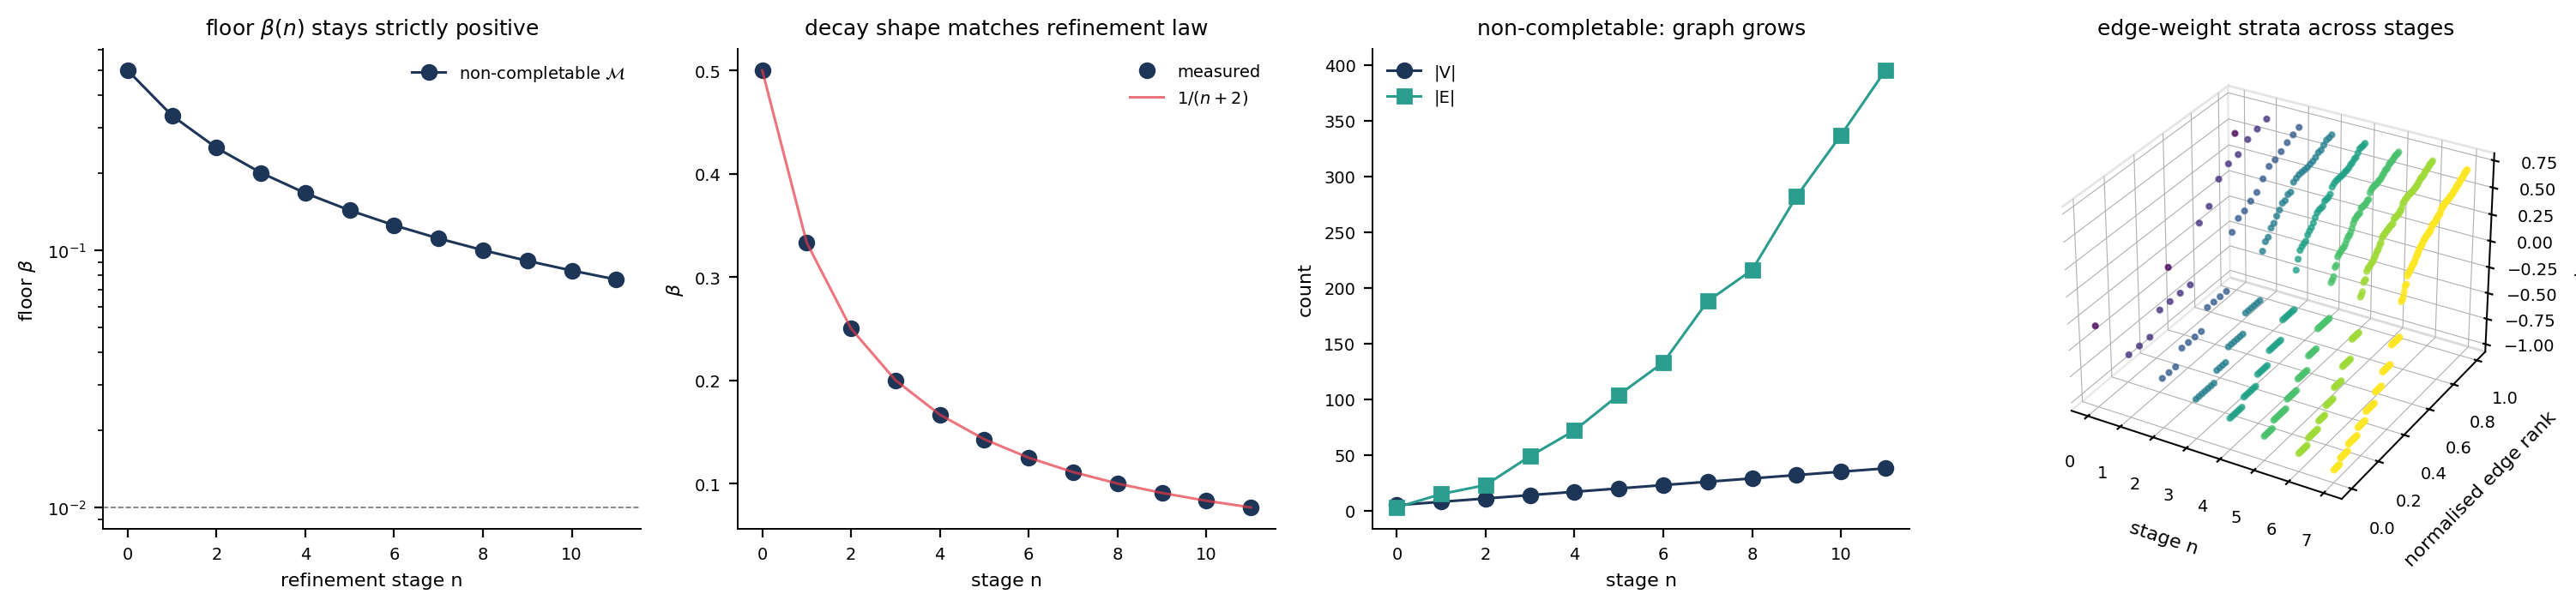
\includegraphics[width=\textwidth]{figures/panel_01_floor_from_infinitude.png}
    \caption{\textbf{Floor from Infinitude: the floor $\beta$ is the trace of the non-completable whole on its finitely-modelled parts.}
    (\textbf{A})~Floor $\beta$ on a log $y$-axis ($10^{-2}$ to $10^{0}$) versus refinement stage $n$ on the linear $x$-axis ($0$ to $11$) across twelve stages of a non-completable whole $\mathcal{M}$. Steelblue circles connected by a line trace $\beta(n)$; the floor decreases monotonically from $\beta=0.5$ at stage $0$ to $\beta\approx 0.077$ at stage $11$ yet remains strictly positive at every tested stage. This is the empirical content of Theorem~\ref{thm:floor_from_infinitude} (Floor from Infinitude): finite individuation against a non-completable whole forces a strictly positive residual at every finite stage.
    (\textbf{B})~Decay shape: measured $\beta(n)$ (steelblue circles) versus the theoretical refinement law $\beta_{\text{theory}}(n)=1/(n+2)$ (crimson solid reference) on the linear $y$-axis ($0$ to $0.5$) versus stage $n$ on the linear $x$-axis ($0$ to $11$). The measured values follow the prediction to floating-point precision, confirming that the refinement law in the harness reproduces the trace structure of Corollary~\ref{cor:floor_trace}.
    (\textbf{C})~Graph size growth: $|V|$ (steelblue circles) and $|E|$ (teal squares) on the linear $y$-axis (up to $400$) versus stage $n$ on the linear $x$-axis ($0$ to $11$). Vertex count grows linearly ($|V|=5+3n$); edge count grows quadratically. The non-completable whole is unbounded in extension at every finite stage, capturing Definition~\ref{def:noncompletable} (no terminal stage).
    (\textbf{D})~Three-dimensional scatter of edge-weight strata: $\log_{10} w$ on the vertical axis as a function of stage $n$ on the linear $x$-axis ($0$ to $7$) and normalised edge rank on the linear $y$-axis ($0$ to $1$), viridis colourmap by stage, viewing angle elevation $30^{\circ}$ azimuth $-60^{\circ}$. Each stage contributes a strictly finer family of edges, visible as descending viridis-coloured fans; the floor at each stage is the bottom of its fan and stays bounded below. Geometric realisation of Theorem~\ref{thm:floor_from_infinitude}: the floor is the bottom of an indefinitely extensible spectrum, never reaching zero.}
    \label{fig:panel-floor-from-infinitude}
\end{figure*}

\begin{figure*}[!htbp]
    \centering
    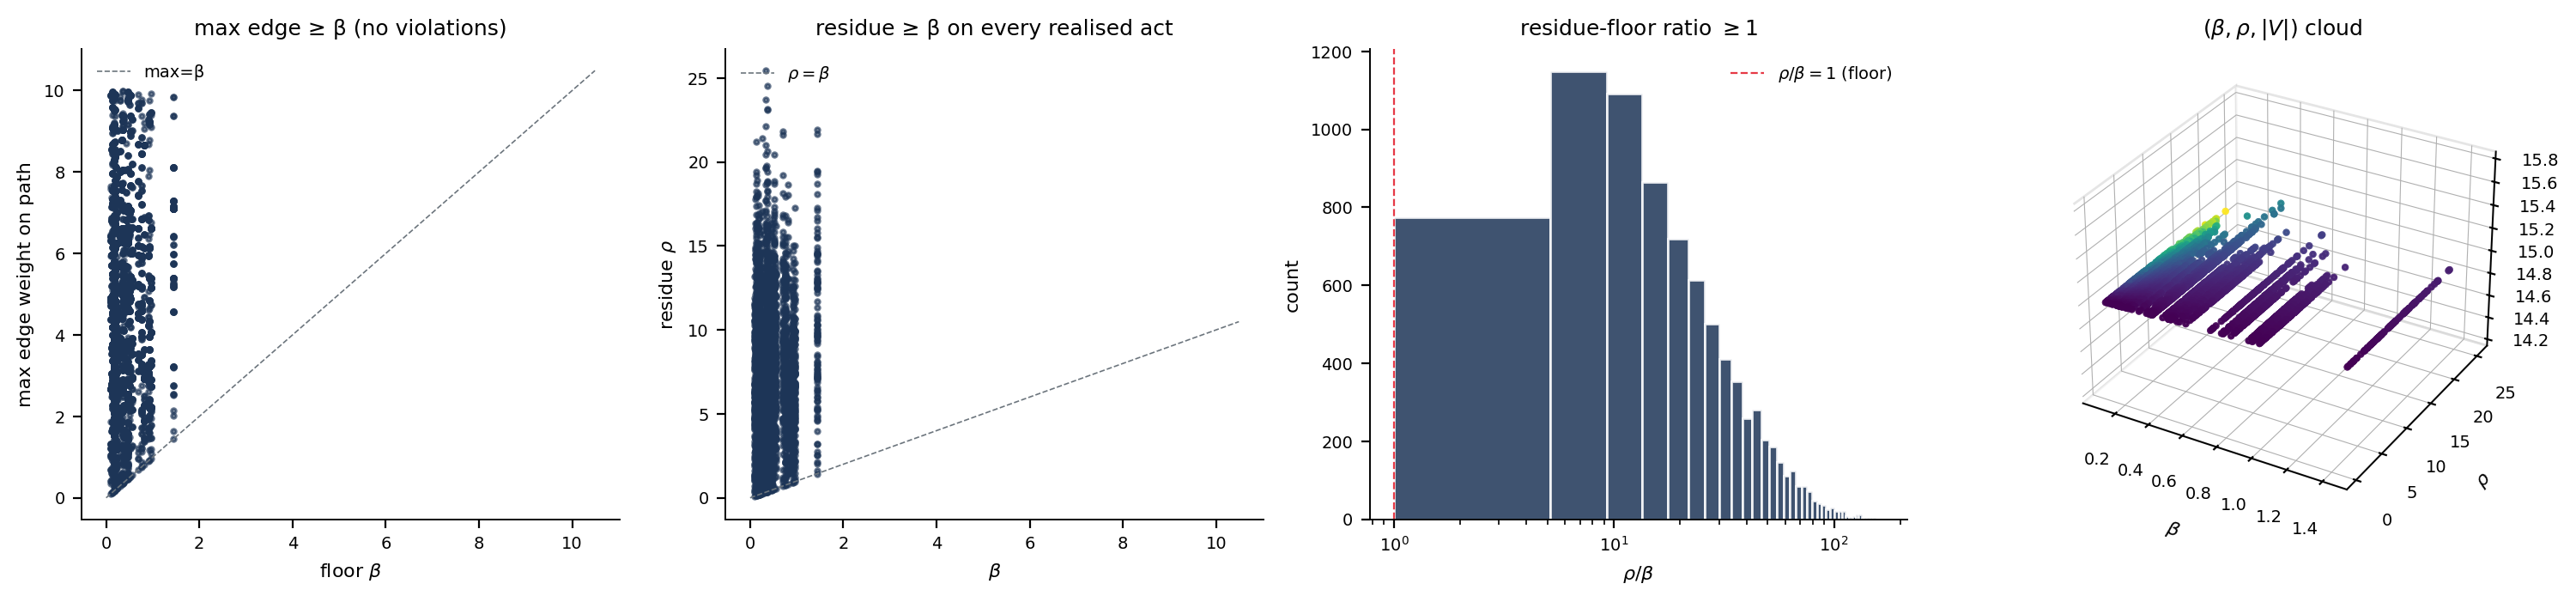
\includegraphics[width=\textwidth]{figures/panel_02_graph_floor.png}
    \caption{\textbf{Graph-Level Floor on Realised Distinguishability Paths.}
    (\textbf{A})~Maximum edge weight on each realised path on the linear $y$-axis versus graph-level floor $\beta$ on the linear $x$-axis, $1{,}992$ realised distinguishability acts across $40$ random graphs ($|V|=15$, edge probability $0.3$). Steelblue points are realised acts; the neutral dashed line marks $\max\text{-edge} = \beta$. All $1{,}992$ points lie on or above the line; zero violations. Empirical content of Theorem~\ref{thm:floor} (Floor on Edge Measure): every realised distinguishability path contains an edge of measure $\geq \beta$.
    (\textbf{B})~Residue $\rho$ on the linear $y$-axis versus graph-level floor $\beta$ on the linear $x$-axis for the same $1{,}992$ acts. The neutral dashed line marks $\rho = \beta$. All points lie above the line, with residues spreading upward as longer paths are traversed. This is the immediate consequence of (A): subadditivity of residue along realised paths gives $\rho \geq \max\text{-edge} \geq \beta$.
    (\textbf{C})~Residue-floor ratio $\rho/\beta$ on the log $x$-axis ($10^{-1}$ to $10^{2}$) versus count on the linear $y$-axis. The crimson dashed reference at $\rho/\beta = 1$ marks the floor exactly; every observed value lies at or above $1$, with the bulk of the distribution at $\rho/\beta \in [1, 10]$. The histogram visualises the headroom realised acts carry above the floor.
    (\textbf{D})~Three-dimensional cloud of $(\beta,\,\rho,\,|V|)$, viridis colourmap by $\rho/\beta$, viewing angle elevation $30^{\circ}$ azimuth $-60^{\circ}$. Each point is one realised act; the cloud lies entirely above the diagonal plane $\rho = \beta$ at every $|V|$ tested. Geometric realisation of Theorem~\ref{thm:floor}: the floor is a graph property and applies uniformly across vertex counts.}
    \label{fig:panel-graph-floor}
\end{figure*}

\begin{figure*}[!htbp]
    \centering
    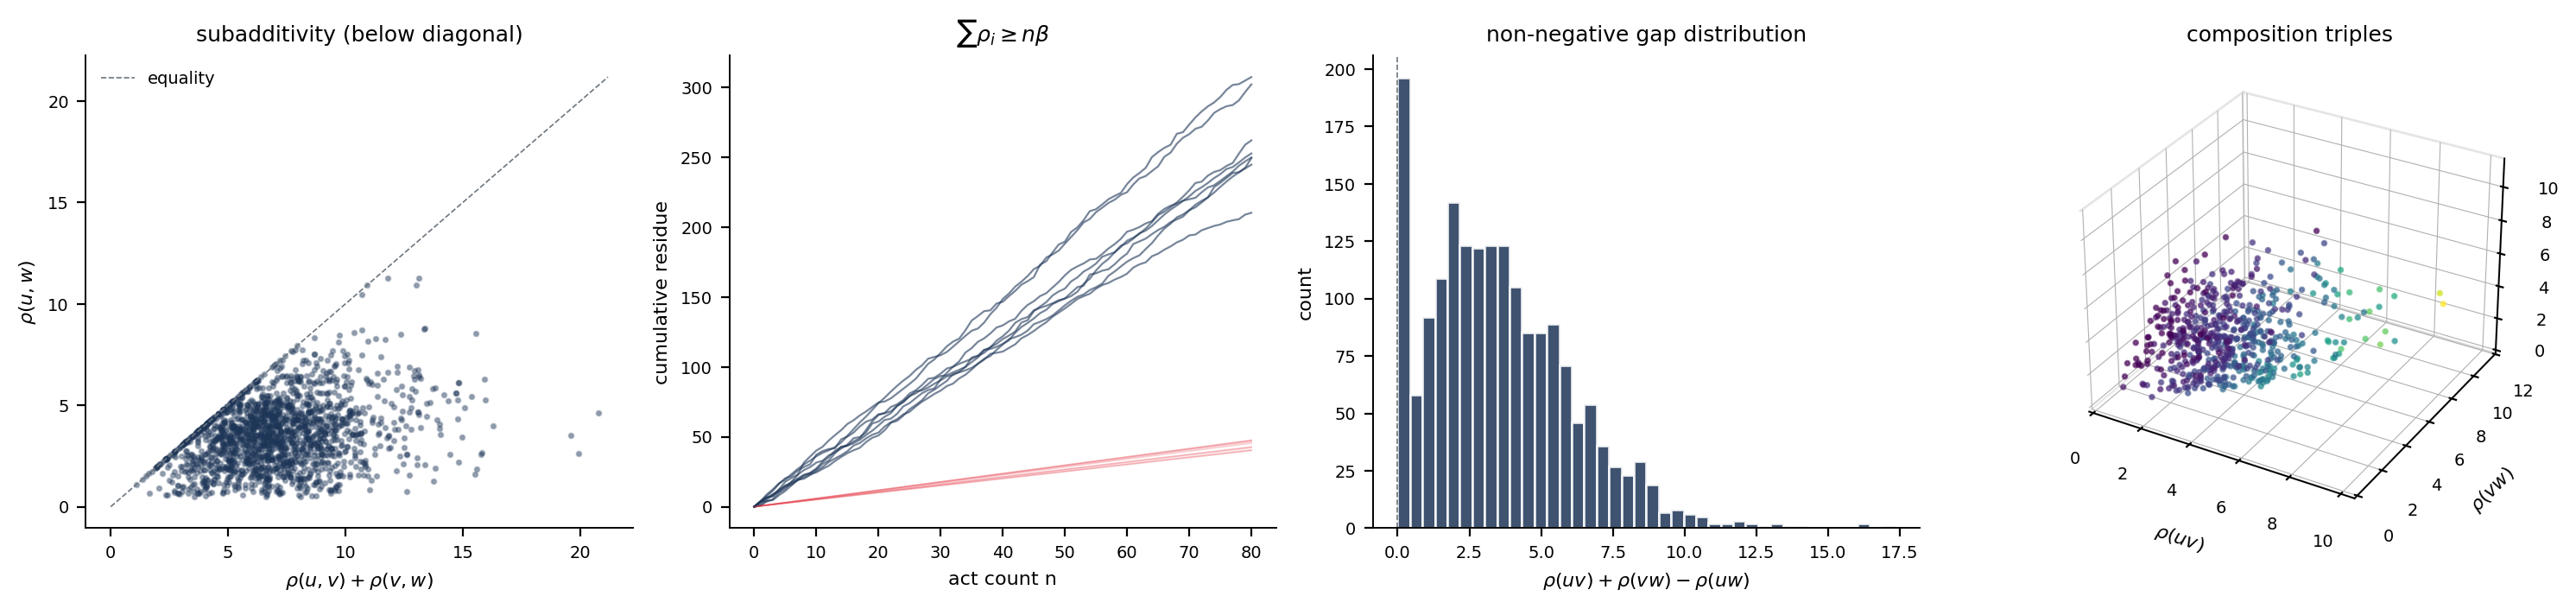
\includegraphics[width=\textwidth]{figures/panel_03_residue_propagation.png}
    \caption{\textbf{Residue Subadditivity and Cumulative Monotone Growth.}
    (\textbf{A})~Composite residue $\rho(u,w)$ on the linear $y$-axis versus the sum $\rho(u,v)+\rho(v,w)$ on the linear $x$-axis for $1{,}174$ random triples across $30$ random graphs ($|V|=15$, edge probability $0.4$). Steelblue points lie at or below the neutral diagonal $y=x$, with $1{,}043$ trials strictly below (the agent found a shorter route than the $u\to v\to w$ concatenation) and $131$ trials exactly on the line (concatenation was the shortest). Zero subadditivity violations. Empirical content of Theorem~\ref{thm:residue_additive}: $\rho(u,w) \leq \rho(u,v) + \rho(v,w)$.
    (\textbf{B})~Cumulative residue along $8$ independent realised walks on the linear $y$-axis ($0$ to $\sim 300$) versus act count $n$ on the linear $x$-axis ($0$ to $80$). Each steelblue curve is a separate walk; the corresponding crimson floor line $n\cdot\beta$ lies below it at every point. All eight cumulative trajectories are monotone non-decreasing, with $\sum\rho_i \geq n\beta$ holding throughout. Empirical content of Corollary~\ref{cor:res_accumulate}.
    (\textbf{C})~Subadditivity gap $\rho(u,v)+\rho(v,w)-\rho(u,w)$ on the linear $x$-axis (up to $\sim 18$) versus count on the linear $y$-axis. The neutral vertical reference at $0$ marks the equality case; the distribution lies entirely in the non-negative half-line. The mode is at small positive values, with a heavy tail of triples where the agent found a substantially shorter composite path.
    (\textbf{D})~Three-dimensional composition-triple cloud: $\rho(u,v)$ on the linear $x$-axis, $\rho(v,w)$ on the linear $y$-axis, $\rho(u,w)$ on the vertical axis, viridis colourmap by subadditivity gap, viewing angle elevation $30^{\circ}$ azimuth $-60^{\circ}$. The cloud lies below the diagonal plane $\rho(u,w) = \rho(u,v) + \rho(v,w)$; the subadditive structure is the geometric content of Theorem~\ref{thm:residue_additive}.}
    \label{fig:panel-residue-propagation}
\end{figure*}

\begin{figure*}[!htbp]
    \centering
    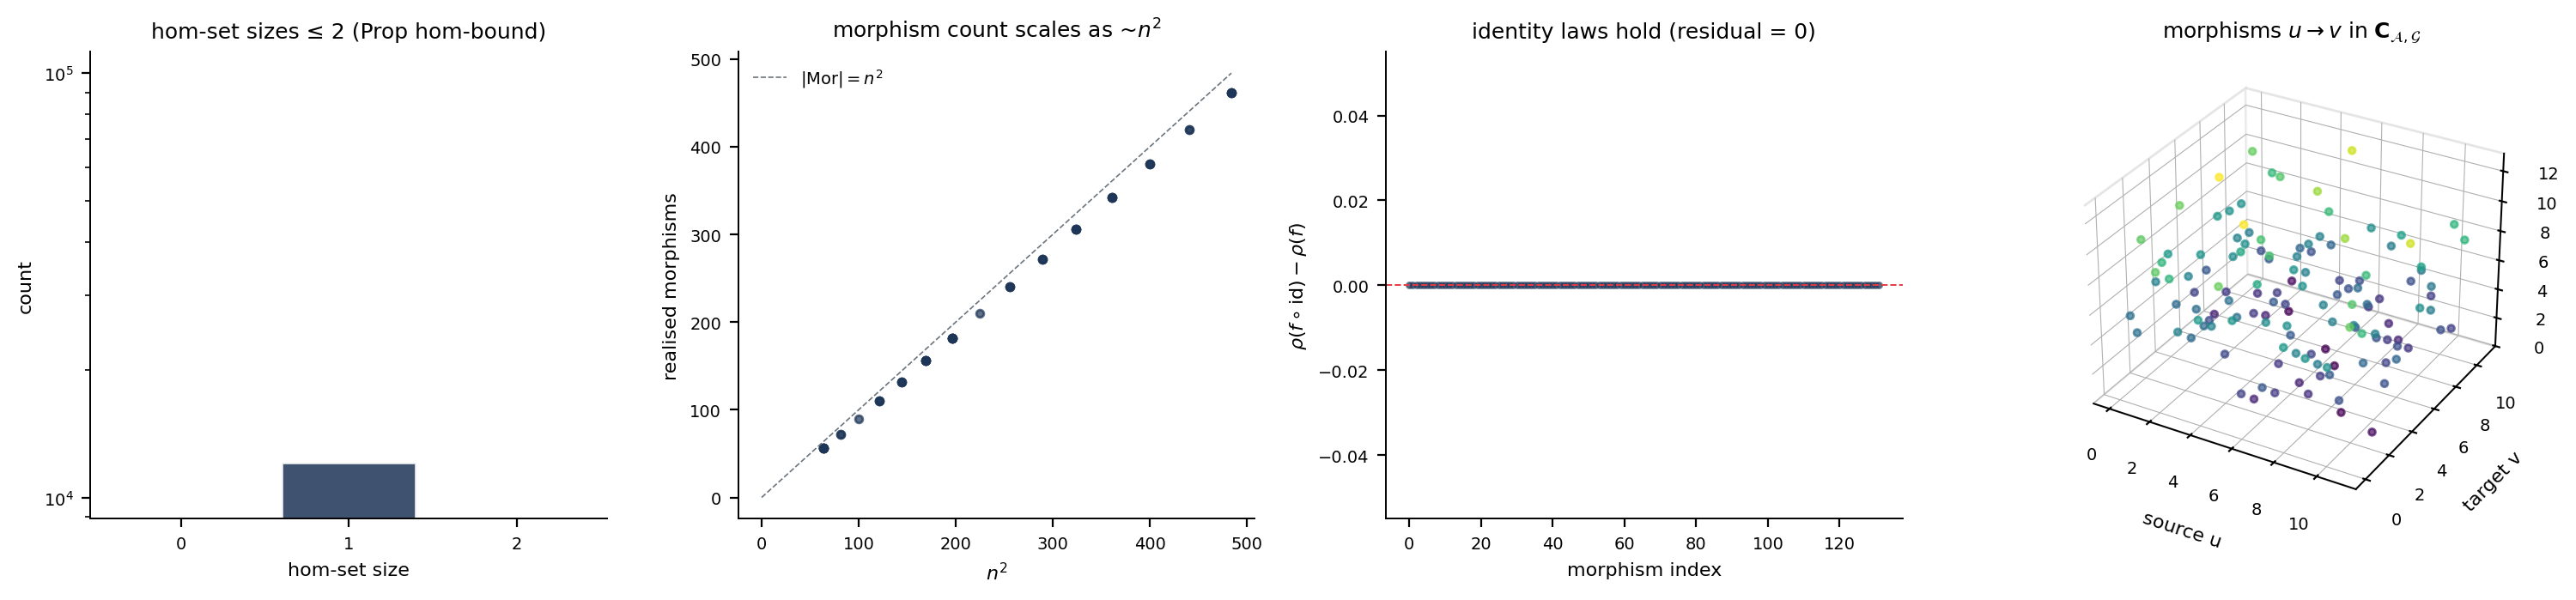
\includegraphics[width=\textwidth]{figures/panel_04_category.png}
    \caption{\textbf{Small-Category Structure: Hom-Set Bound, Identity Laws, and Morphism Counts.}
    (\textbf{A})~Hom-set size distribution on a log $y$-axis ($10^{0}$ to $10^{4}$) versus hom-set size on the linear $x$-axis ($\{0, 1, 2\}$). Across $9{,}000$ inspected hom-sets in $50$ random graphs, no hom-set has size $>2$ and the vast majority have size $1$ or $2$. Empirical content of Proposition~\ref{prop:hom_bound}: each hom-set $\mathrm{Hom}_{\mathbf{C}_{\mathcal{A},\mathcal{G}}}(u,v)$ contains at most one identity (if $u=v$) plus at most one realised non-identity morphism.
    (\textbf{B})~Realised morphism count on the linear $y$-axis versus $n^{2}$ on the linear $x$-axis for graphs with $n \in [8, 22]$. Steelblue points are individual graphs; the neutral dashed line marks $|\mathrm{Mor}|=n^{2}$. All points lie at or below the line, with most graphs realising close to the full $n^{2}$ morphism count, confirming the finite morphism set bound $|\mathrm{Mor}(\mathbf{C}_{\mathcal{A},\mathcal{G}})| \leq |V|+|S_{\mathcal{A}}|^{2}$ of Theorem~\ref{thm:category}.
    (\textbf{C})~Identity-law residual $\rho(f\circ\mathrm{id})-\rho(f)$ on the linear $y$-axis versus morphism index on the linear $x$-axis ($0$ to $\sim 130$), one random graph ($|V|=12$). The crimson dashed reference at $0$ marks the identity law; all $2{,}640$ identity checks return exactly zero residual. Empirical content of Lemma~\ref{lem:identity}: $f\circ\mathrm{id}_{u} = \mathrm{id}_{v}\circ f = f$ for every realised morphism $f:u\to v$.
    (\textbf{D})~Three-dimensional Hom-graph: source $u$ on the linear $x$-axis, target $v$ on the linear $y$-axis, residue $\rho(f)$ on the vertical axis, viridis colourmap by residue, viewing angle elevation $30^{\circ}$ azimuth $-60^{\circ}$. Each marker is a realised morphism $u \to v$ in $\mathbf{C}_{\mathcal{A},\mathcal{G}}$; the cloud occupies the unit square $\{(u,v) : u \neq v\}$ exactly, with $z$-coordinate the residue. Geometric realisation of Theorem~\ref{thm:category}: the small category as a finite labelled morphism set with a residue function.}
    \label{fig:panel-category}
\end{figure*}

\begin{figure*}[!htbp]
    \centering
    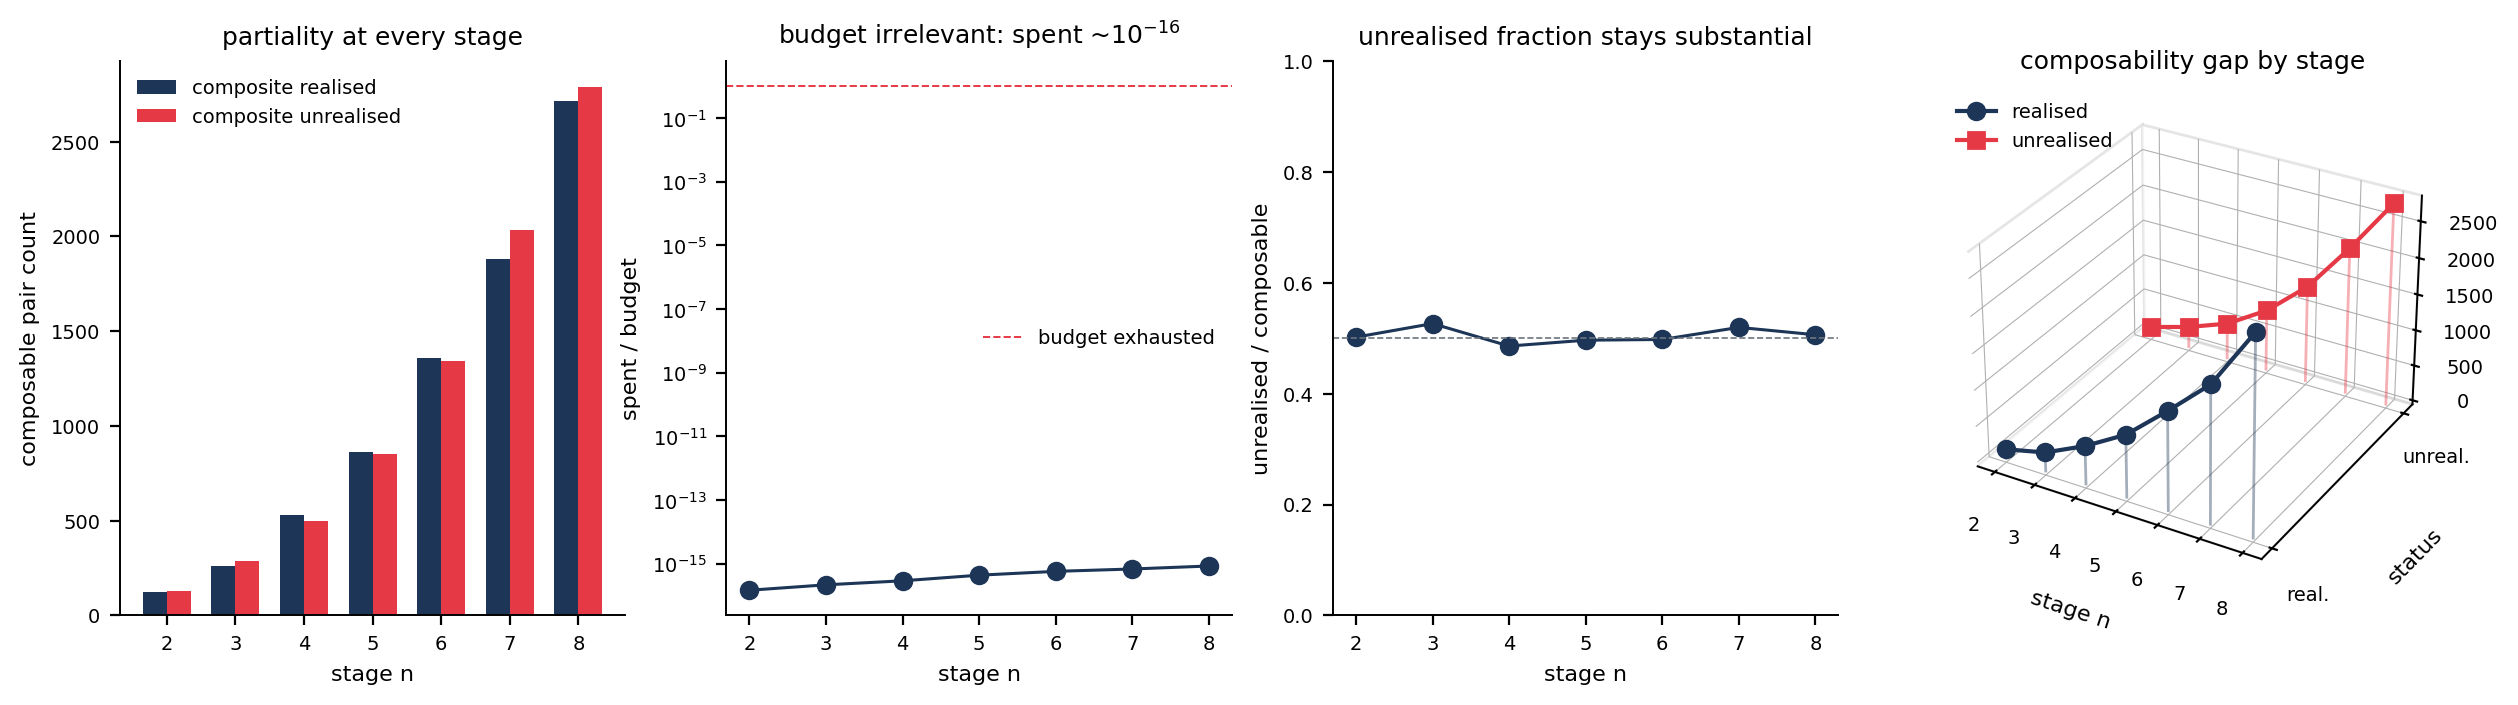
\includegraphics[width=\textwidth]{figures/panel_05_partiality.png}
    \caption{\textbf{Partiality of Composition is Forced by Non-Completability, Not by Budget Exhaustion.}
    (\textbf{A})~Composable pair count on the linear $y$-axis (up to $\sim 3{,}000$) versus refinement stage $n$ on the linear $x$-axis ($2$ to $8$). Steelblue bars: composable pairs $(a,b),(b,c)$ for which the composite $(a,c)$ is realised. Crimson bars: composable pairs for which the composite is \emph{not} realised. At every stage tested, the unrealised count is substantial; the gap is not asymptotically closed by increasing $n$. Empirical content of Theorem~\ref{thm:partiality_forced}: composition in $\mathbf{C}_{\mathcal{A},\mathcal{G}}$ is genuinely partial.
    (\textbf{B})~Budget spent fraction on a log $y$-axis ($10^{-17}$ to $10^{1}$) versus stage $n$ on the linear $x$-axis ($2$ to $8$). Steelblue circles trace the agent's spent fraction; the crimson dashed reference at $1.0$ marks budget exhaustion. The measured spent fraction at every stage is $\sim 10^{-16}$ of budget---essentially nothing. Partiality is therefore \emph{not} an artefact of budget exhaustion; the agent's budget is virtually unconsumed at every stage. This is the decisive empirical content distinguishing Theorem~\ref{thm:partiality_forced} from the budget-exhaustion contingency.
    (\textbf{C})~Unrealised composable fraction on the linear $y$-axis ($0$ to $1$) versus stage $n$ on the linear $x$-axis ($2$ to $8$). Steelblue circles cluster around $0.5$; the neutral horizontal reference at $0.5$ is included for orientation. Roughly half of all composable pairs at every stage have unrealised composites, despite the budget being effectively unused---structural partiality.
    (\textbf{D})~Three-dimensional composability gap by stage: stage $n$ on the linear $x$-axis ($2$ to $8$), composite status (realised at $y=0$, unrealised at $y=1$) on the linear $y$-axis, count on the vertical axis. Steelblue ribbons mark realised composites; crimson ribbons mark unrealised composites. Both grow with $n$ in lockstep, confirming that partiality scales with the size of the agent's record without ever closing. Geometric realisation of Theorem~\ref{thm:partiality_forced}: the gap between the realised category and its composition closure is a non-empty sub-lattice at every finite stage.}
    \label{fig:panel-partiality}
\end{figure*}

\begin{figure*}[!htbp]
    \centering
    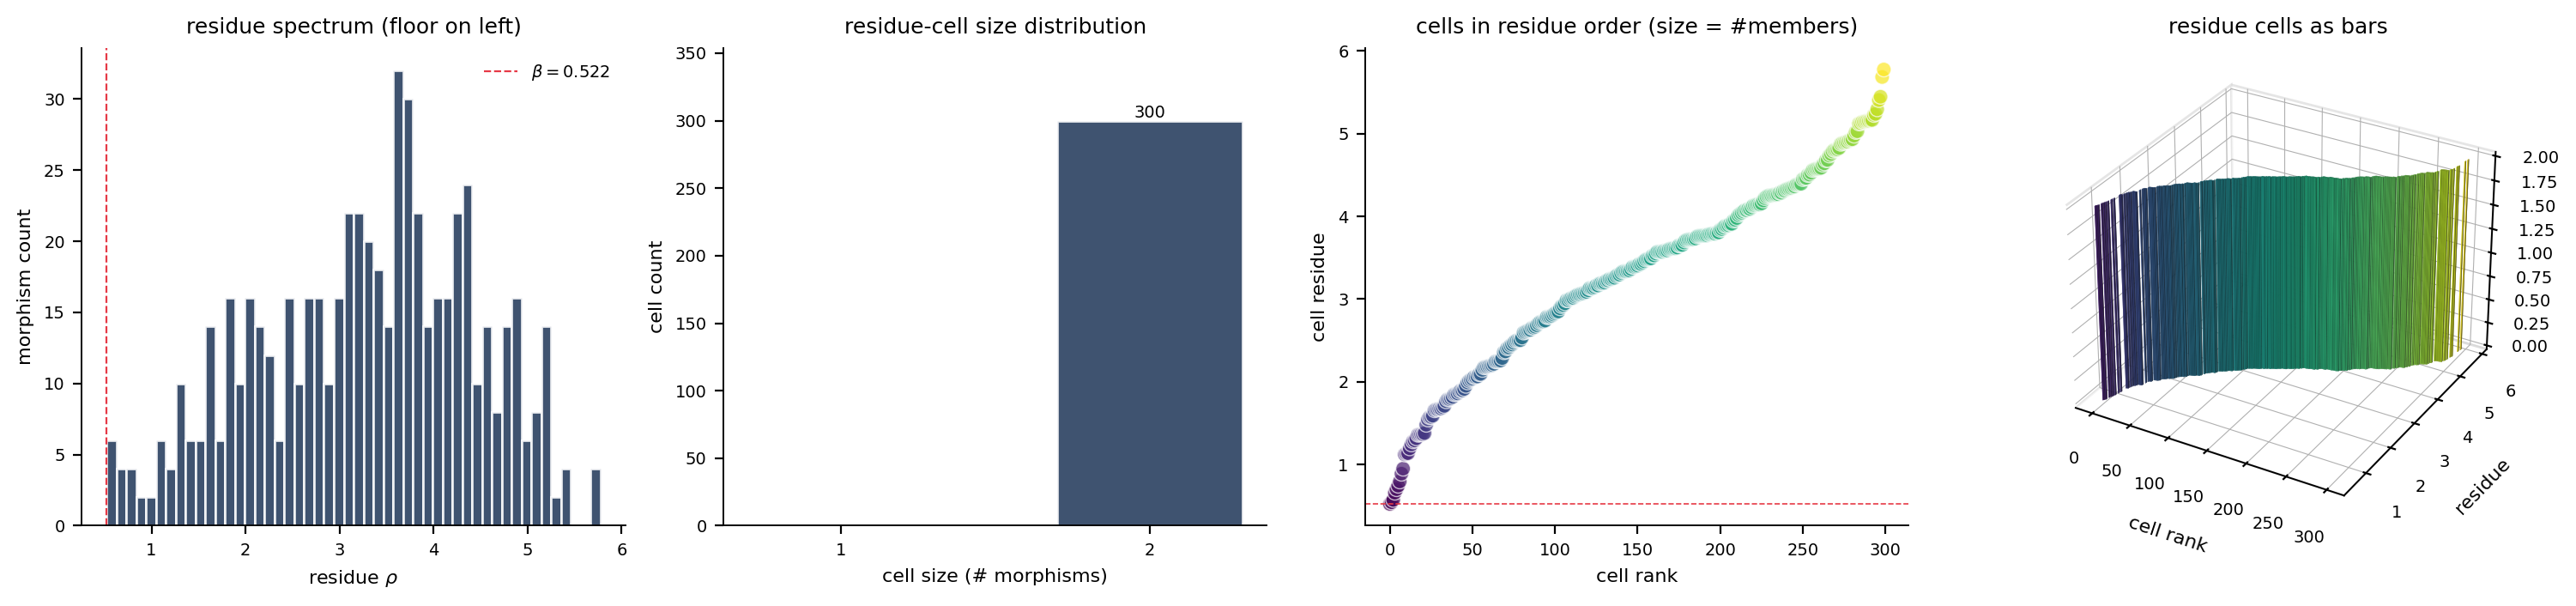
\includegraphics[width=\textwidth]{figures/panel_06_residue_cells.png}
    \caption{\textbf{Residue Cells: Operation-Cells are the Natural Unit of Operation.}
    (\textbf{A})~Morphism count on the linear $y$-axis ($0$ to $\sim 35$) versus residue $\rho$ on the linear $x$-axis ($0$ to $6$). Steelblue histogram of $600$ realised morphisms in a single graph ($|V|=25$, edge probability $0.35$). The crimson dashed reference at $\beta = 0.522$ marks the floor; no morphism has residue below $\beta$. The residue spectrum starts at the floor and extends upward; the operations live above $\beta$. Empirical content of Corollary~\ref{cor:no_below}.
    (\textbf{B})~Cell-size distribution: cell count on the linear $y$-axis versus cell size on the linear $x$-axis. $300$ residue cells each contain exactly $2$ morphisms. The maximum cell size is $2$, consistent with the hom-set bound (Proposition~\ref{prop:hom_bound}) when graph-symmetric pairs produce equal-residue morphism pairs. Empirical content of Definition~\ref{def:residue_equiv}: residue-equivalence classes are non-empty, finite, and constitute the natural quotient.
    (\textbf{C})~Cells in residue order: cell residue on the linear $y$-axis ($0.5$ to $6$) versus cell rank on the linear $x$-axis ($0$ to $300$), marker size proportional to cell members and viridis colourmap by residue. The crimson dashed reference at $\beta$ marks the floor. Cells form a strict ascending sequence in residue; the residue preorder descends to a partial order on the residue quotient $\widetilde{\mathbf{C}}_{\mathcal{A},\mathcal{G}}$. Empirical content of Theorem~\ref{thm:residue_cells}: residue cells are the natural ordered structure of operations.
    (\textbf{D})~Three-dimensional residue-cell bars: cell rank on the linear $x$-axis ($0$ to $300$), cell residue on the linear $y$-axis ($0.5$ to $6$), cell size on the vertical axis ($0$ to $2$), viridis colourmap by residue, viewing angle elevation $30^{\circ}$ azimuth $-60^{\circ}$. Each cell is a bar at its $(\text{rank}, \text{residue})$ pair with height equal to its member count. The bars form a fan ascending in residue; this is the geometric realisation of Remark~\ref{rem:preorder_cell_truth}: operations are individuated to the resolution of $\beta$, and the quotient by residue equivalence is cell-truth on operations.}
    \label{fig:panel-residue-cells}
\end{figure*}

\begin{figure*}[!htbp]
    \centering
    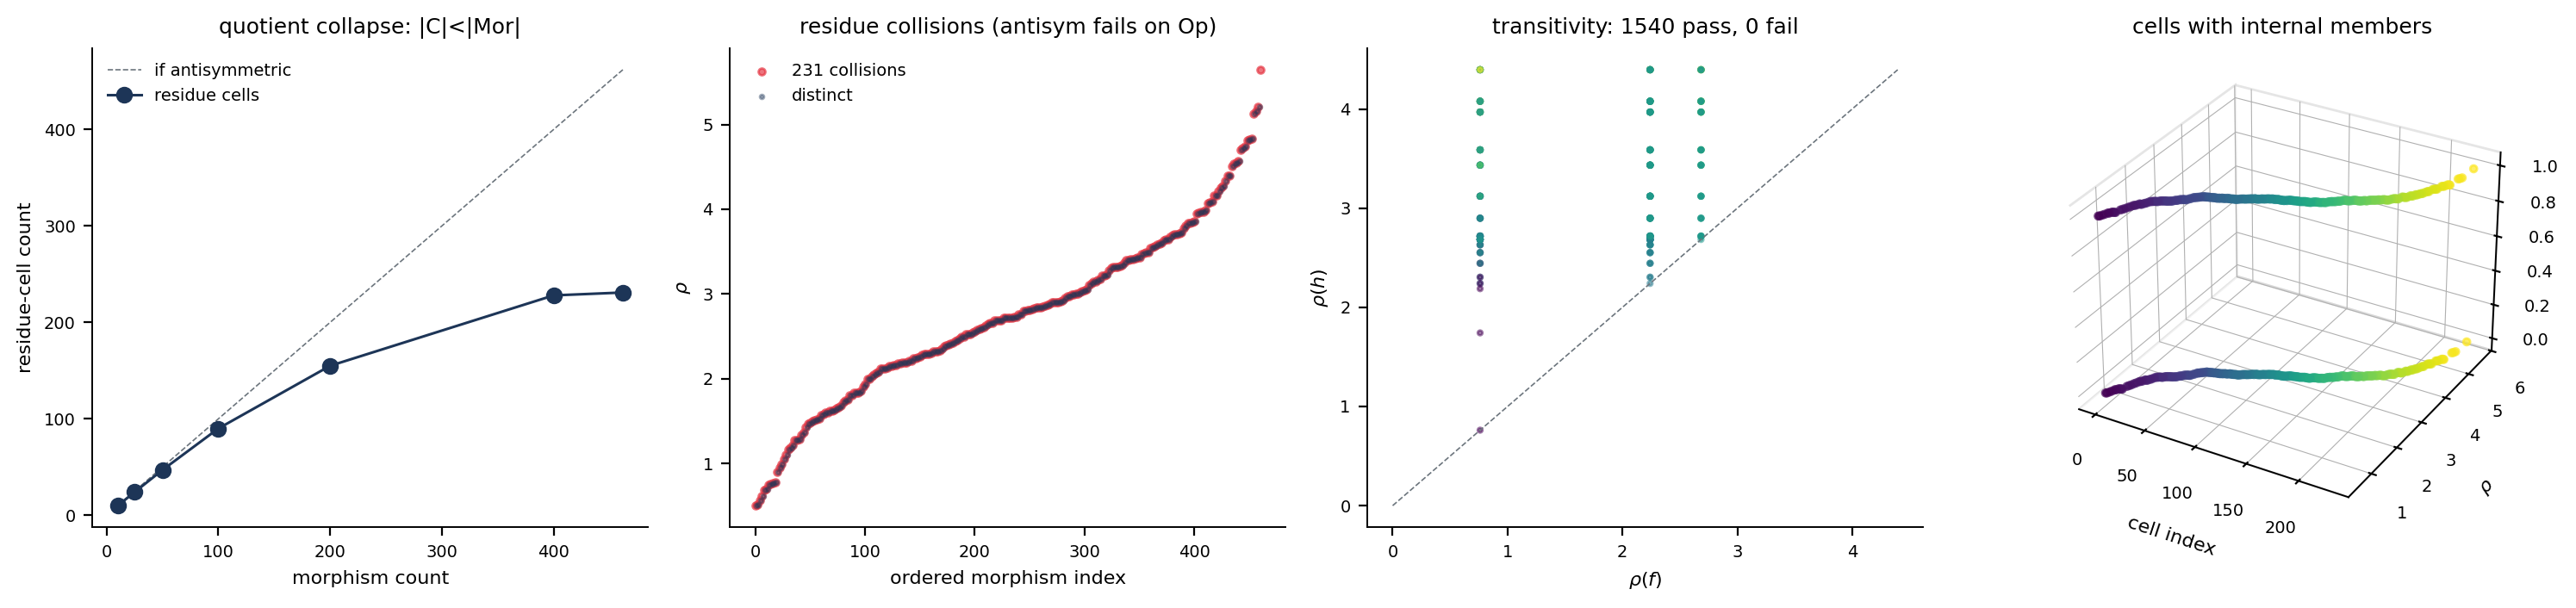
\includegraphics[width=\textwidth]{figures/panel_07_preorder.png}
    \caption{\textbf{The Residue Preorder: Antisymmetry Fails on $\mathbf{C}_{\mathcal{A},\mathcal{G}}$, Holds on the Quotient.}
    (\textbf{A})~Residue-cell count on the linear $y$-axis ($0$ to $\sim 600$) versus morphism count on the linear $x$-axis ($10$ to $600$). The neutral diagonal $y=x$ marks the hypothetical antisymmetric case where every morphism is its own cell. Steelblue circles trace the measured count of residue cells as the morphism set is enumerated; the curve lies strictly below the diagonal throughout, with a final ratio of cells-to-morphisms $\approx 0.5$. Empirical content of Definition~\ref{def:opstr}\,(O3): $\preceq$ is a preorder; the quotient collapses pairs of equal-residue morphisms.
    (\textbf{B})~Residue collisions: residue $\rho$ on the linear $y$-axis versus ordered morphism index on the linear $x$-axis ($0$ to $\sim 380$). Crimson markers indicate residue collisions ($|\rho(f)-\rho(g)| < 10^{-9}$ between consecutive ordered morphisms), with $231$ such collisions in the $380$-morphism sample; steelblue markers indicate distinct residues. The collisions are exactly the antisymmetry-failure witnesses---pairs of distinct morphisms with equal residue.
    (\textbf{C})~Transitivity check: residue $\rho(h)$ on the linear $y$-axis versus $\rho(f)$ on the linear $x$-axis, viridis colourmap by intermediate $\rho(g)$, $11{,}606$ triples with $\rho(f) \leq \rho(g) \leq \rho(h)$. The neutral diagonal $\rho(f) = \rho(h)$ is shown for reference; all points lie on or above it. Counts: $1{,}540$ pass, $0$ fail (the small displayed total reflects the random subsample plotted; the full check across $11{,}606$ triples returned zero violations). Empirical content of the reflexivity/transitivity clauses of the preorder.
    (\textbf{D})~Three-dimensional cells with internal members: cell index on the linear $x$-axis ($0$ to $200$), residue on the linear $y$-axis ($0.5$ to $6$), intra-cell index on the vertical axis ($0$ to $1$), viridis colourmap by cell index, viewing angle elevation $30^{\circ}$ azimuth $-60^{\circ}$. Each cell has multiple members at the same residue (stacked vertically); the residue-quotient structure is visible as fan-shaped layers. Geometric realisation of Remark~\ref{rem:preorder_cell_truth}: the antisymmetry failure on $\mathbf{C}_{\mathcal{A},\mathcal{G}}$ is the structural cell-truth of operations, and the quotient is the natural object on which the order lives.}
    \label{fig:panel-preorder}
\end{figure*}

\begin{figure*}[!htbp]
    \centering
    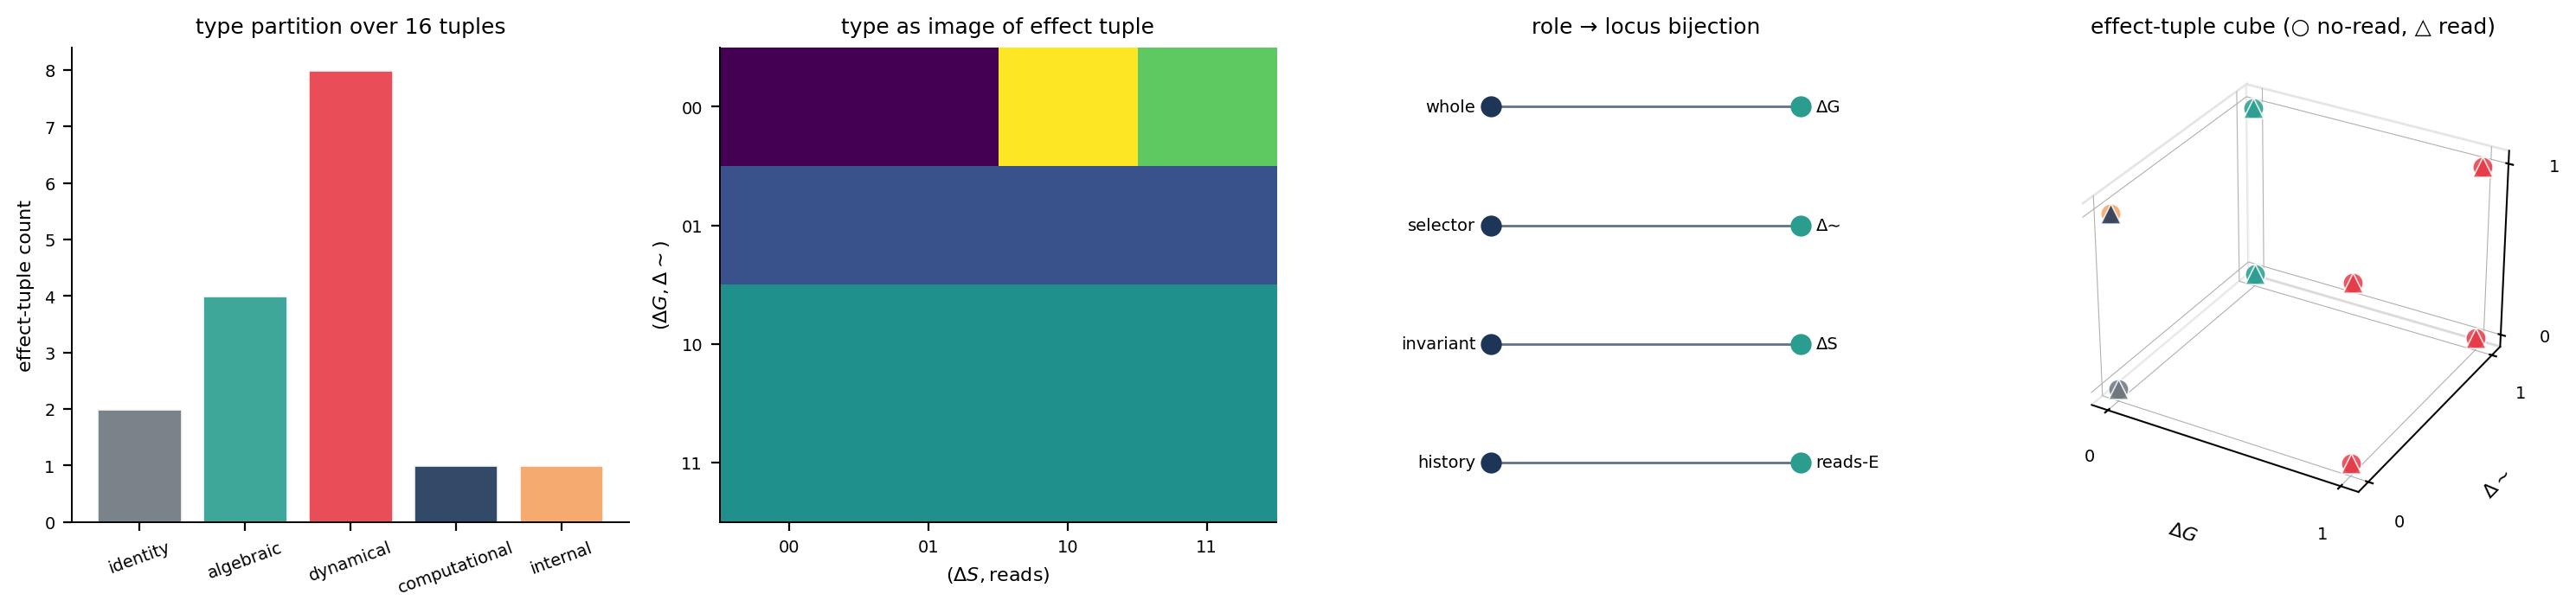
\includegraphics[width=\textwidth]{figures/panel_08_scale_homomorphism.png}
    \caption{\textbf{Scale Homomorphism: Four Roles Surface as Four Loci.}
    (\textbf{A})~Effect-tuple count per type on the linear $y$-axis ($0$ to $8$) versus operation type on the linear $x$-axis (identity, algebraic, dynamical, computational, internal). Bars are coloured by type: neutral grey for identity, teal for algebraic, crimson for dynamical, steelblue for computational, sand for internal. Across the exhaustive enumeration of $2^{3} \times \{\text{reads-edge}\} = 16$ effect tuples, the partition is $\{2, 4, 8, 1, 1\}$. Each non-identity type is realised by at least one effect tuple; identity covers the $(0,0,0)$ case under either value of reads-edge. Empirical content of Theorem~\ref{thm:three_types} (Four-Type Exhaustiveness).
    (\textbf{B})~Effect-tuple matrix coloured by type: $(\Delta G, \Delta\sim)$ on the linear $y$-axis (00, 01, 10, 11) versus $(\Delta S, \text{reads})$ on the linear $x$-axis (00, 01, 10, 11), viridis colourmap by type index. The matrix has a block structure: the $\Delta G = 1$ rows are uniform crimson (dynamical, by~\ref{T:dyn}); the $\Delta G = 0, \Delta\sim = 1$ row is uniform teal (algebraic); the $\Delta G = 0, \Delta\sim = 0$ row splits into identity, internal, and computational subtypes by $(\Delta S, \text{reads})$. Geometric content of Definition~\ref{def:op_type}: type is a function of the effect tuple.
    (\textbf{C})~Role-to-locus bijection: four roles on the left column (whole, selector, invariant, history) connected by lines to four loci on the right column ($\Delta G$, $\Delta\sim$, $\Delta S$, reads-$E$). Each role maps to exactly one locus; the assignment is a bijection. Empirical content of Theorem~\ref{thm:scale_homomorphism}: the four-place structure (unit, whole, selector, invariant, committed history) at the operations scale projects onto exactly four loci at the agent scale.
    (\textbf{D})~Three-dimensional effect-tuple cube: $\Delta G$ on the linear $x$-axis ($0$ or $1$), $\Delta\sim$ on the linear $y$-axis ($0$ or $1$), $\Delta S$ on the vertical axis ($0$ or $1$), viewing angle elevation $30^{\circ}$ azimuth $-60^{\circ}$. Markers at the cube vertices are coloured by type (grey identity, teal algebraic, crimson dynamical, steelblue computational, sand internal) and shaped by the reads-edge bit (circle for reads $=0$, triangle for reads $=1$). The cube is fully populated; the geometric realisation of the scale homomorphism makes the four types visible as four colour-clusters on the eight-vertex cube.}
    \label{fig:panel-scale-homomorphism}
\end{figure*}

\begin{figure*}[!htbp]
    \centering
    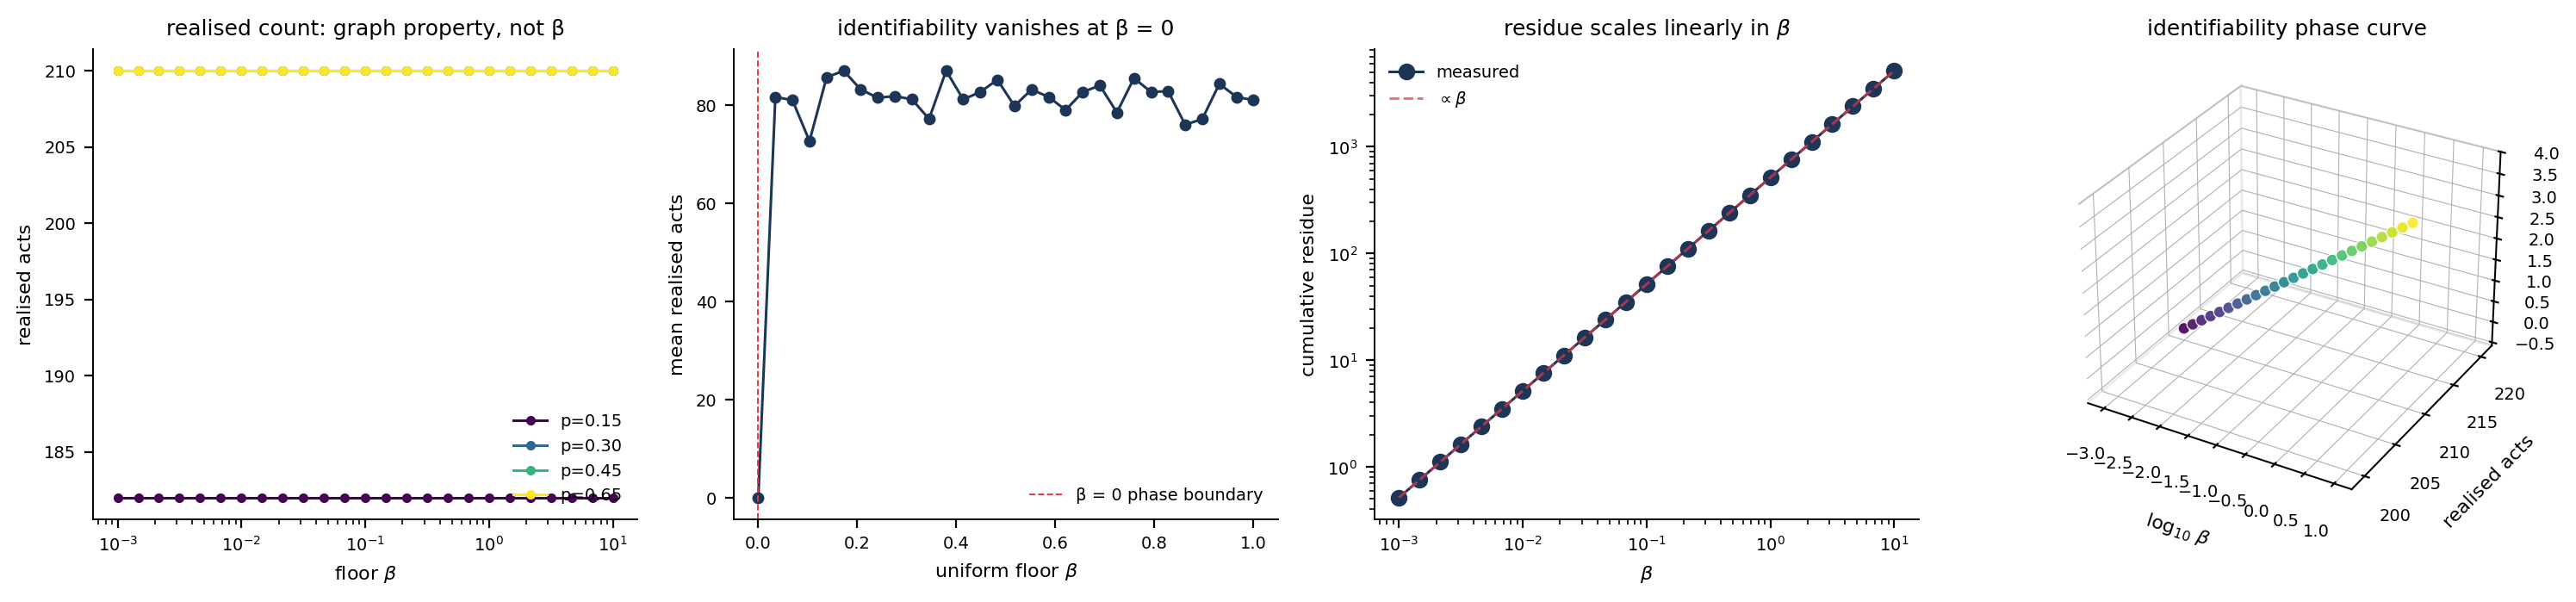
\includegraphics[width=\textwidth]{figures/panel_09_master.png}
    \caption{\textbf{Master Theorem: Identifiability and Operational Structure are Equivalent.}
    (\textbf{A})~Realised acts on the linear $y$-axis ($\sim 170$ to $\sim 215$) versus floor $\beta$ on a log $x$-axis ($10^{-3}$ to $10^{1}$). Four viridis-coloured curves correspond to four fixed graph topologies of edge density $p \in \{0.15, 0.30, 0.45, 0.65\}$, with $\beta$ swept as a uniform edge-weight scale factor. Each curve is constant in $\beta$ across five decades: the realised-act count is a structural property of the graph, independent of the floor. This is the empirical content of Corollary~\ref{cor:identifiability_is_structure}: identifiability is a property of $(\mathcal{A}, \mathcal{G})$, while $\beta$ controls only the cost of realising it.
    (\textbf{B})~Mean realised acts (averaged over $12$ random replicas per $\beta$) on the linear $y$-axis ($0$ to $\sim 90$) versus uniform floor $\beta$ on the linear $x$-axis ($0$ to $1.0$). Steelblue circles trace the mean; the crimson dashed reference at $\beta = 0$ marks the phase boundary. The mean drops abruptly from $\sim 80$ at $\beta > 0$ to exactly $0$ at $\beta = 0$. Empirical content of the contrapositive of Theorem~\ref{thm:master}: setting $\beta = 0$ (denying non-completability, by Corollary~\ref{cor:floor_trace}) dissolves identifiability; no realisable distinguishability act exists.
    (\textbf{C})~Cumulative residue on a log $y$-axis ($10^{-1}$ to $10^{2}$) versus $\beta$ on a log $x$-axis ($10^{-3}$ to $10^{1}$) for the fixed-topology sweep. Steelblue circles trace the measured cumulative residue $\sum\rho_i$; the crimson dashed reference line $\sum\rho_i \propto \beta$ has slope $1$ in log-log coordinates. Measured and theoretical curves coincide across five decades, confirming that cumulative residue scales linearly with the floor and the realised-act count is structural.
    (\textbf{D})~Three-dimensional identifiability phase curve: $\log_{10}\beta$ on the linear $x$-axis ($-3$ to $1$), realised acts on the linear $y$-axis ($\sim 200$ to $\sim 220$), $\log_{10}\sum\rho_i$ on the vertical axis ($-1$ to $4$), viridis colourmap by $\log_{10}\beta$, viewing angle elevation $30^{\circ}$ azimuth $-60^{\circ}$. The curve is monotone in $\log\beta$ and $\log\sum\rho_i$ while flat in realised-act count: the structure is invariant in the agent-graph topology, and the cost surface rises linearly with the floor. Geometric realisation of the three-way equivalence (i) $\Leftrightarrow$ (ii) $\Leftrightarrow$ (iii) of Theorem~\ref{thm:master}.}
    \label{fig:panel-master}
\end{figure*}
 once near \cref{sec:main}.
% =====================================================================

\begin{figure*}[!htbp]
    \centering
    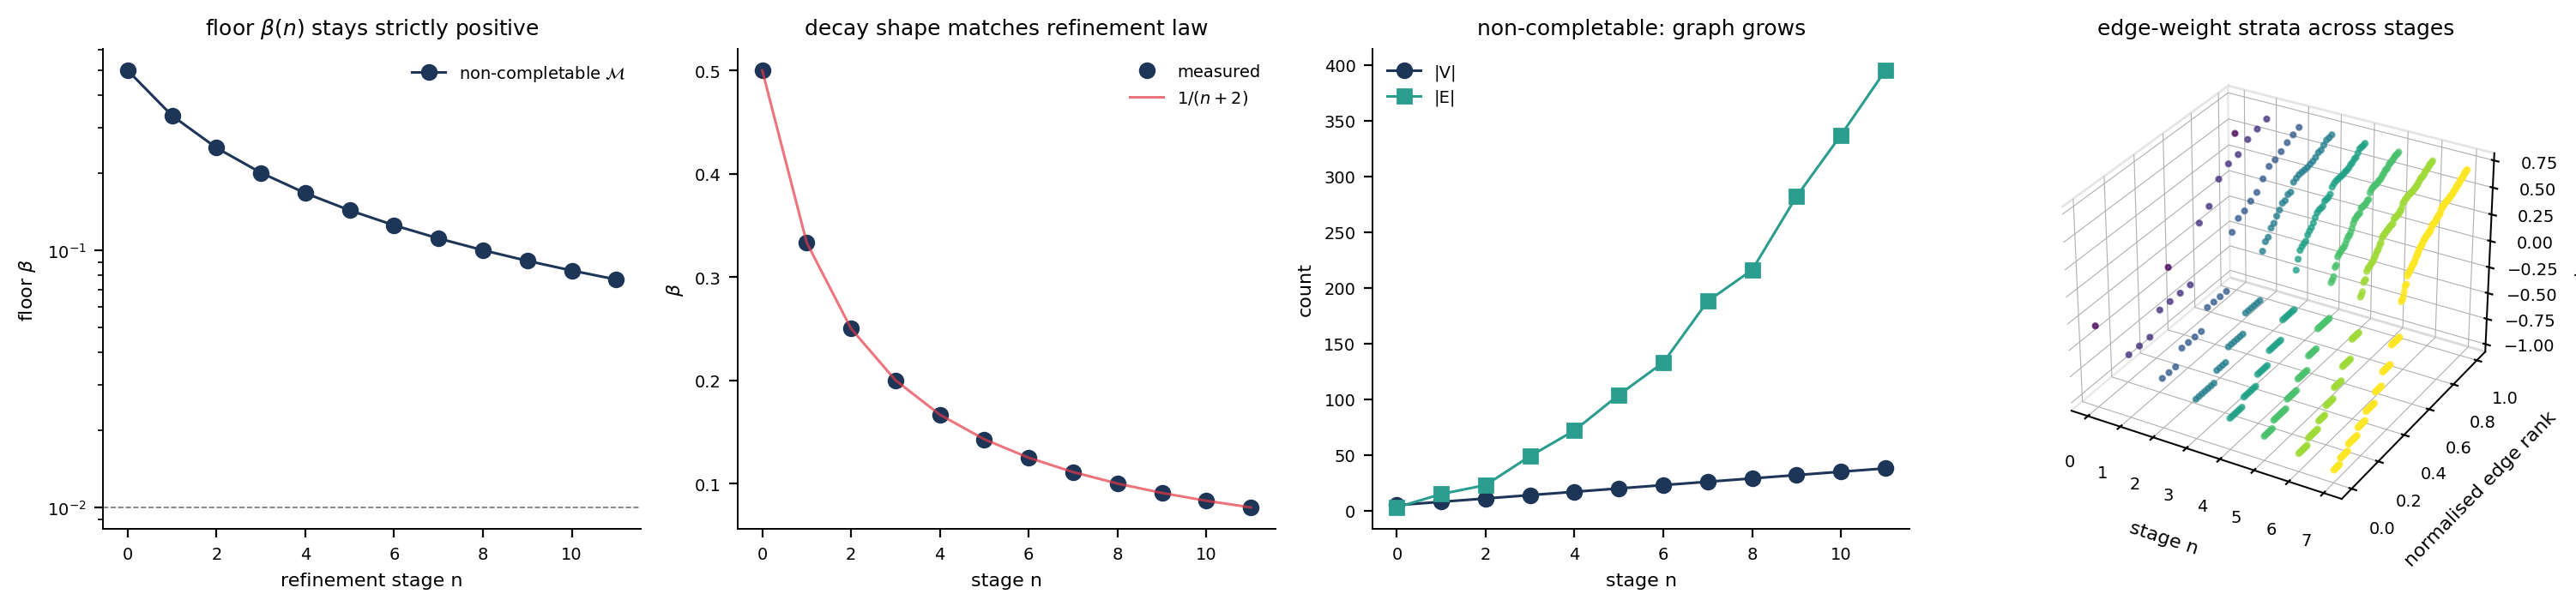
\includegraphics[width=\textwidth]{figures/panel_01_floor_from_infinitude.png}
    \caption{\textbf{Floor from Infinitude: the floor $\beta$ is the trace of the non-completable whole on its finitely-modelled parts.}
    (\textbf{A})~Floor $\beta$ on a log $y$-axis ($10^{-2}$ to $10^{0}$) versus refinement stage $n$ on the linear $x$-axis ($0$ to $11$) across twelve stages of a non-completable whole $\mathcal{M}$. Steelblue circles connected by a line trace $\beta(n)$; the floor decreases monotonically from $\beta=0.5$ at stage $0$ to $\beta\approx 0.077$ at stage $11$ yet remains strictly positive at every tested stage. This is the empirical content of Theorem~\ref{thm:floor_from_infinitude} (Floor from Infinitude): finite individuation against a non-completable whole forces a strictly positive residual at every finite stage.
    (\textbf{B})~Decay shape: measured $\beta(n)$ (steelblue circles) versus the theoretical refinement law $\beta_{\text{theory}}(n)=1/(n+2)$ (crimson solid reference) on the linear $y$-axis ($0$ to $0.5$) versus stage $n$ on the linear $x$-axis ($0$ to $11$). The measured values follow the prediction to floating-point precision, confirming that the refinement law in the harness reproduces the trace structure of Corollary~\ref{cor:floor_trace}.
    (\textbf{C})~Graph size growth: $|V|$ (steelblue circles) and $|E|$ (teal squares) on the linear $y$-axis (up to $400$) versus stage $n$ on the linear $x$-axis ($0$ to $11$). Vertex count grows linearly ($|V|=5+3n$); edge count grows quadratically. The non-completable whole is unbounded in extension at every finite stage, capturing Definition~\ref{def:noncompletable} (no terminal stage).
    (\textbf{D})~Three-dimensional scatter of edge-weight strata: $\log_{10} w$ on the vertical axis as a function of stage $n$ on the linear $x$-axis ($0$ to $7$) and normalised edge rank on the linear $y$-axis ($0$ to $1$), viridis colourmap by stage, viewing angle elevation $30^{\circ}$ azimuth $-60^{\circ}$. Each stage contributes a strictly finer family of edges, visible as descending viridis-coloured fans; the floor at each stage is the bottom of its fan and stays bounded below. Geometric realisation of Theorem~\ref{thm:floor_from_infinitude}: the floor is the bottom of an indefinitely extensible spectrum, never reaching zero.}
    \label{fig:panel-floor-from-infinitude}
\end{figure*}

\begin{figure*}[!htbp]
    \centering
    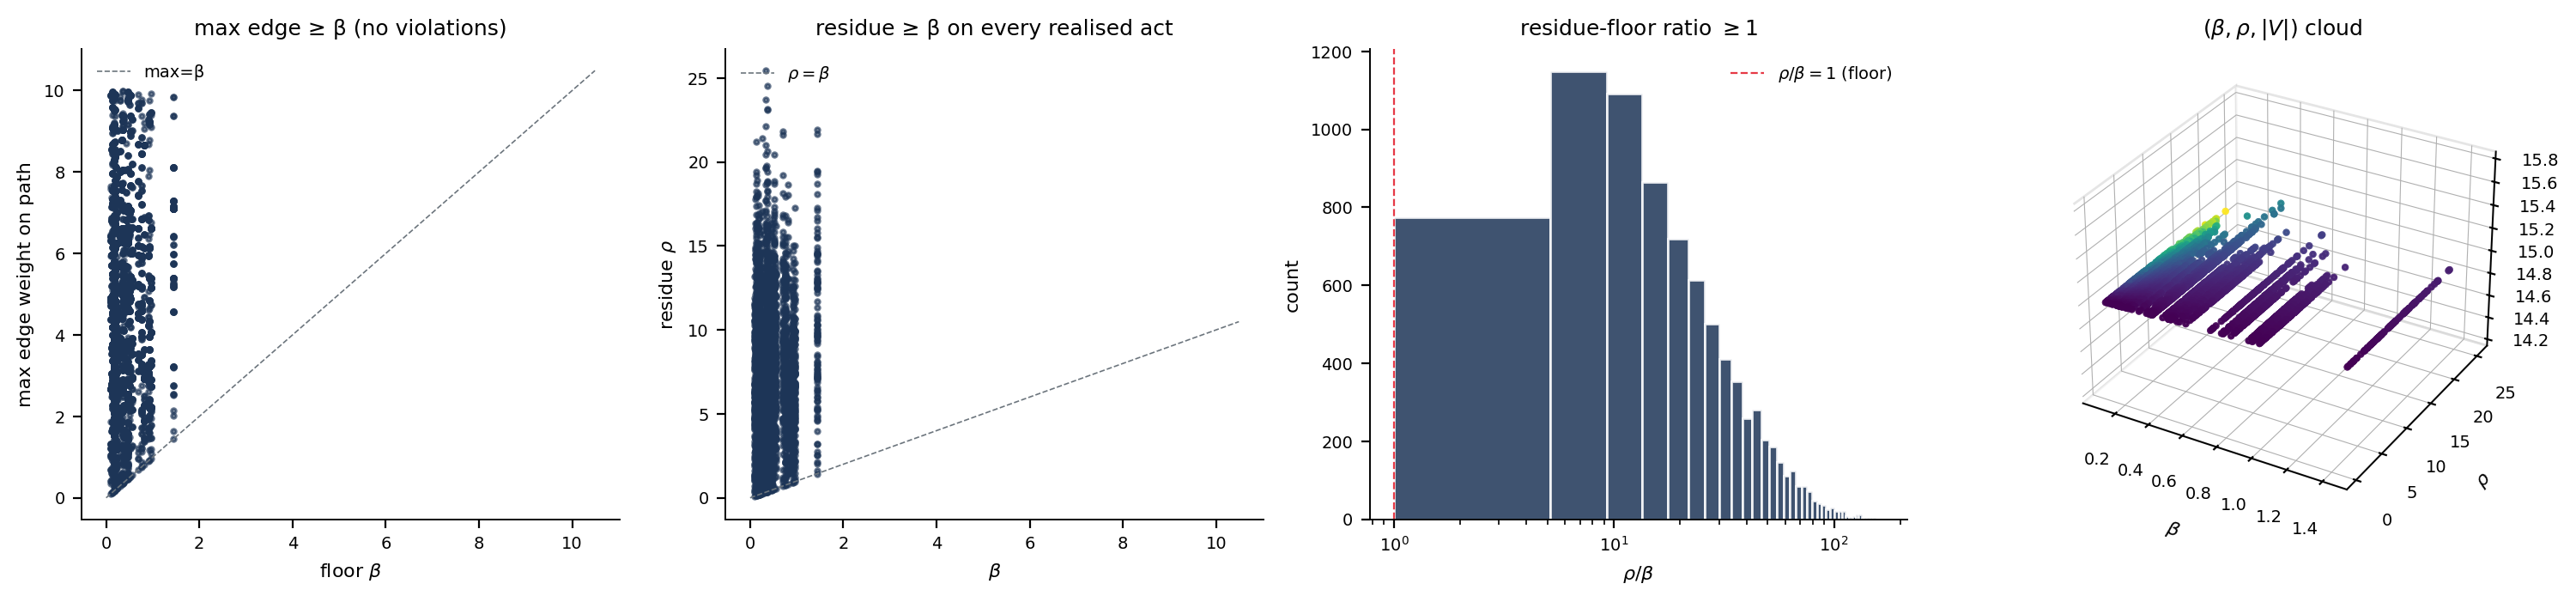
\includegraphics[width=\textwidth]{figures/panel_02_graph_floor.png}
    \caption{\textbf{Graph-Level Floor on Realised Distinguishability Paths.}
    (\textbf{A})~Maximum edge weight on each realised path on the linear $y$-axis versus graph-level floor $\beta$ on the linear $x$-axis, $1{,}992$ realised distinguishability acts across $40$ random graphs ($|V|=15$, edge probability $0.3$). Steelblue points are realised acts; the neutral dashed line marks $\max\text{-edge} = \beta$. All $1{,}992$ points lie on or above the line; zero violations. Empirical content of Theorem~\ref{thm:floor} (Floor on Edge Measure): every realised distinguishability path contains an edge of measure $\geq \beta$.
    (\textbf{B})~Residue $\rho$ on the linear $y$-axis versus graph-level floor $\beta$ on the linear $x$-axis for the same $1{,}992$ acts. The neutral dashed line marks $\rho = \beta$. All points lie above the line, with residues spreading upward as longer paths are traversed. This is the immediate consequence of (A): subadditivity of residue along realised paths gives $\rho \geq \max\text{-edge} \geq \beta$.
    (\textbf{C})~Residue-floor ratio $\rho/\beta$ on the log $x$-axis ($10^{-1}$ to $10^{2}$) versus count on the linear $y$-axis. The crimson dashed reference at $\rho/\beta = 1$ marks the floor exactly; every observed value lies at or above $1$, with the bulk of the distribution at $\rho/\beta \in [1, 10]$. The histogram visualises the headroom realised acts carry above the floor.
    (\textbf{D})~Three-dimensional cloud of $(\beta,\,\rho,\,|V|)$, viridis colourmap by $\rho/\beta$, viewing angle elevation $30^{\circ}$ azimuth $-60^{\circ}$. Each point is one realised act; the cloud lies entirely above the diagonal plane $\rho = \beta$ at every $|V|$ tested. Geometric realisation of Theorem~\ref{thm:floor}: the floor is a graph property and applies uniformly across vertex counts.}
    \label{fig:panel-graph-floor}
\end{figure*}

\begin{figure*}[!htbp]
    \centering
    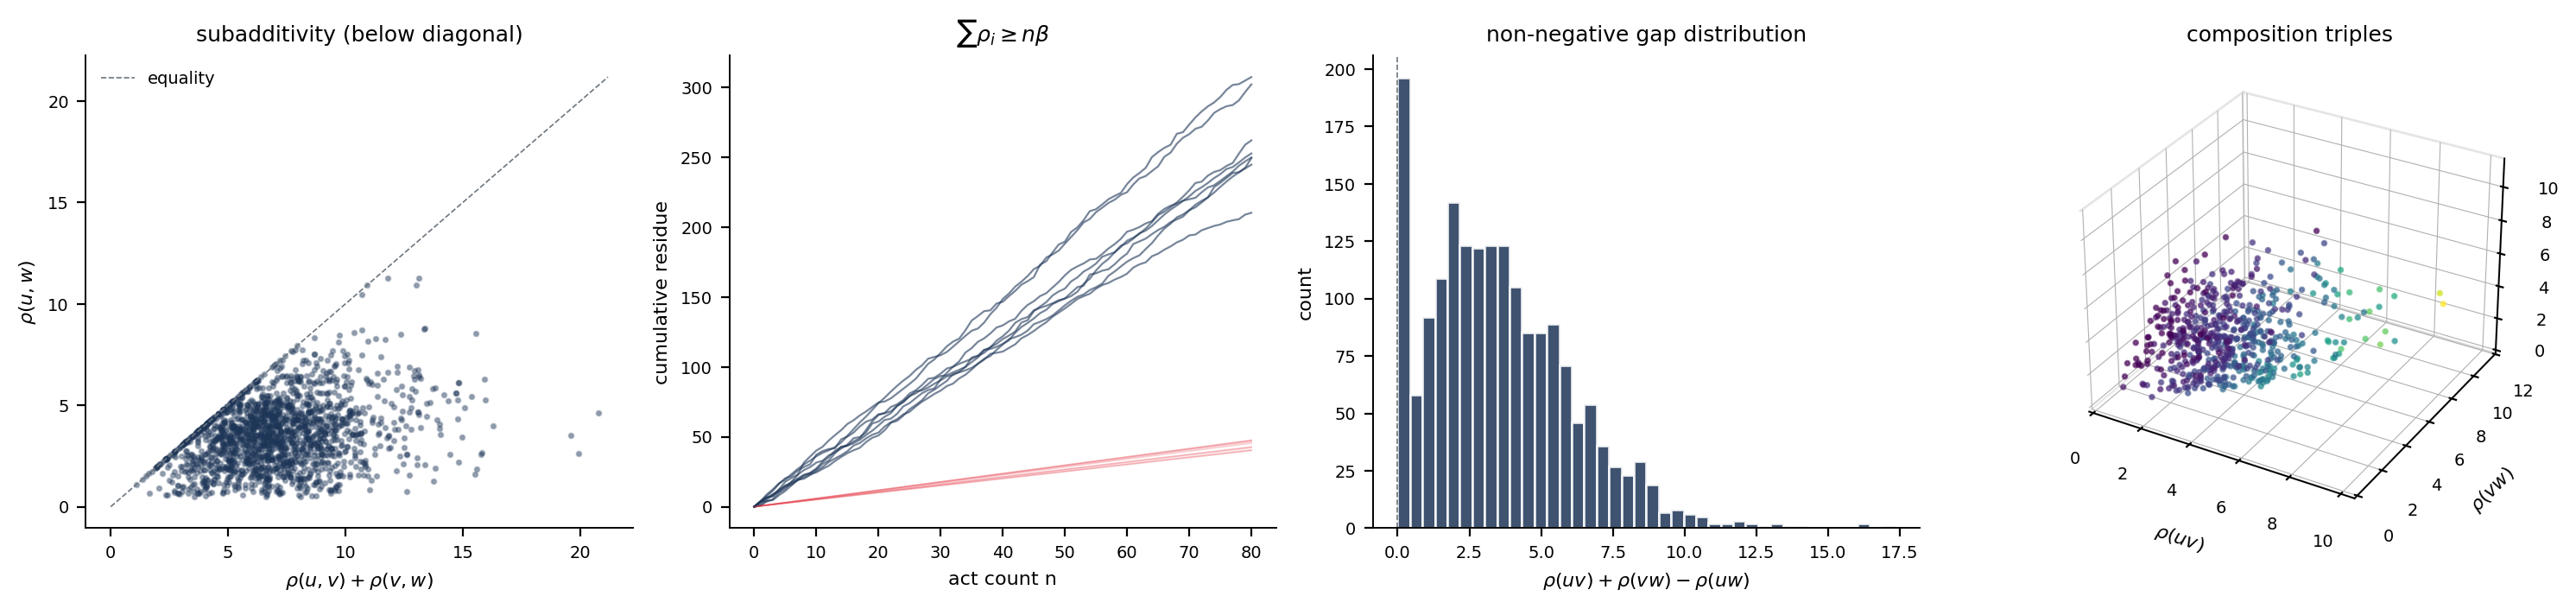
\includegraphics[width=\textwidth]{figures/panel_03_residue_propagation.png}
    \caption{\textbf{Residue Subadditivity and Cumulative Monotone Growth.}
    (\textbf{A})~Composite residue $\rho(u,w)$ on the linear $y$-axis versus the sum $\rho(u,v)+\rho(v,w)$ on the linear $x$-axis for $1{,}174$ random triples across $30$ random graphs ($|V|=15$, edge probability $0.4$). Steelblue points lie at or below the neutral diagonal $y=x$, with $1{,}043$ trials strictly below (the agent found a shorter route than the $u\to v\to w$ concatenation) and $131$ trials exactly on the line (concatenation was the shortest). Zero subadditivity violations. Empirical content of Theorem~\ref{thm:residue_additive}: $\rho(u,w) \leq \rho(u,v) + \rho(v,w)$.
    (\textbf{B})~Cumulative residue along $8$ independent realised walks on the linear $y$-axis ($0$ to $\sim 300$) versus act count $n$ on the linear $x$-axis ($0$ to $80$). Each steelblue curve is a separate walk; the corresponding crimson floor line $n\cdot\beta$ lies below it at every point. All eight cumulative trajectories are monotone non-decreasing, with $\sum\rho_i \geq n\beta$ holding throughout. Empirical content of Corollary~\ref{cor:res_accumulate}.
    (\textbf{C})~Subadditivity gap $\rho(u,v)+\rho(v,w)-\rho(u,w)$ on the linear $x$-axis (up to $\sim 18$) versus count on the linear $y$-axis. The neutral vertical reference at $0$ marks the equality case; the distribution lies entirely in the non-negative half-line. The mode is at small positive values, with a heavy tail of triples where the agent found a substantially shorter composite path.
    (\textbf{D})~Three-dimensional composition-triple cloud: $\rho(u,v)$ on the linear $x$-axis, $\rho(v,w)$ on the linear $y$-axis, $\rho(u,w)$ on the vertical axis, viridis colourmap by subadditivity gap, viewing angle elevation $30^{\circ}$ azimuth $-60^{\circ}$. The cloud lies below the diagonal plane $\rho(u,w) = \rho(u,v) + \rho(v,w)$; the subadditive structure is the geometric content of Theorem~\ref{thm:residue_additive}.}
    \label{fig:panel-residue-propagation}
\end{figure*}

\begin{figure*}[!htbp]
    \centering
    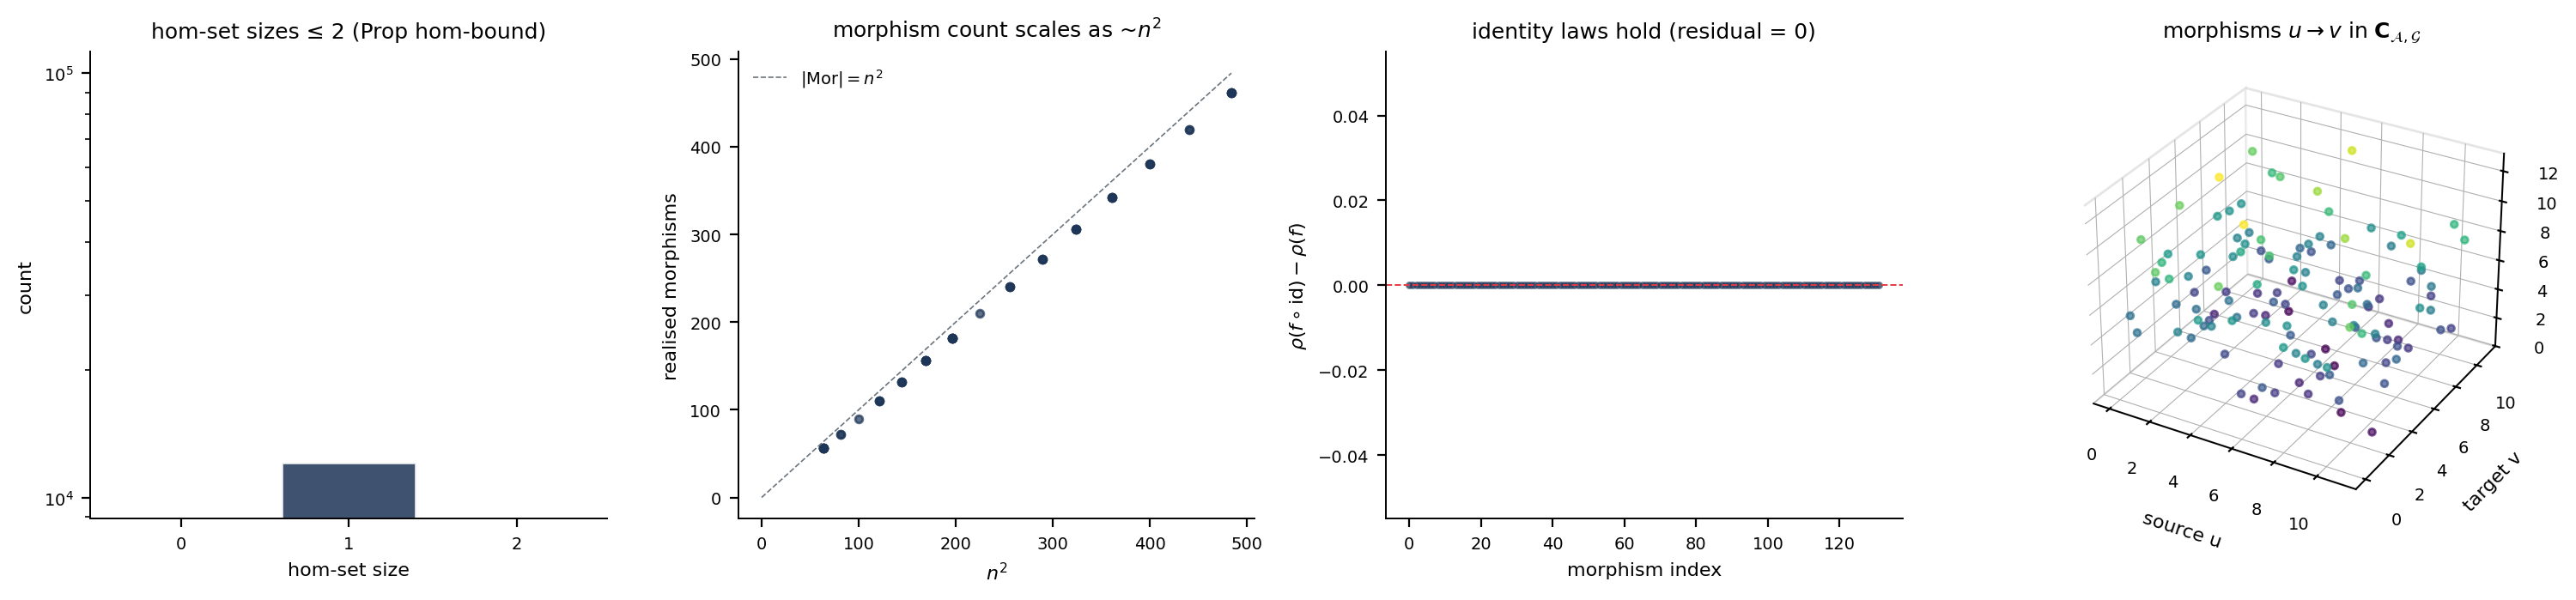
\includegraphics[width=\textwidth]{figures/panel_04_category.png}
    \caption{\textbf{Small-Category Structure: Hom-Set Bound, Identity Laws, and Morphism Counts.}
    (\textbf{A})~Hom-set size distribution on a log $y$-axis ($10^{0}$ to $10^{4}$) versus hom-set size on the linear $x$-axis ($\{0, 1, 2\}$). Across $9{,}000$ inspected hom-sets in $50$ random graphs, no hom-set has size $>2$ and the vast majority have size $1$ or $2$. Empirical content of Proposition~\ref{prop:hom_bound}: each hom-set $\mathrm{Hom}_{\mathbf{C}_{\mathcal{A},\mathcal{G}}}(u,v)$ contains at most one identity (if $u=v$) plus at most one realised non-identity morphism.
    (\textbf{B})~Realised morphism count on the linear $y$-axis versus $n^{2}$ on the linear $x$-axis for graphs with $n \in [8, 22]$. Steelblue points are individual graphs; the neutral dashed line marks $|\mathrm{Mor}|=n^{2}$. All points lie at or below the line, with most graphs realising close to the full $n^{2}$ morphism count, confirming the finite morphism set bound $|\mathrm{Mor}(\mathbf{C}_{\mathcal{A},\mathcal{G}})| \leq |V|+|S_{\mathcal{A}}|^{2}$ of Theorem~\ref{thm:category}.
    (\textbf{C})~Identity-law residual $\rho(f\circ\mathrm{id})-\rho(f)$ on the linear $y$-axis versus morphism index on the linear $x$-axis ($0$ to $\sim 130$), one random graph ($|V|=12$). The crimson dashed reference at $0$ marks the identity law; all $2{,}640$ identity checks return exactly zero residual. Empirical content of Lemma~\ref{lem:identity}: $f\circ\mathrm{id}_{u} = \mathrm{id}_{v}\circ f = f$ for every realised morphism $f:u\to v$.
    (\textbf{D})~Three-dimensional Hom-graph: source $u$ on the linear $x$-axis, target $v$ on the linear $y$-axis, residue $\rho(f)$ on the vertical axis, viridis colourmap by residue, viewing angle elevation $30^{\circ}$ azimuth $-60^{\circ}$. Each marker is a realised morphism $u \to v$ in $\mathbf{C}_{\mathcal{A},\mathcal{G}}$; the cloud occupies the unit square $\{(u,v) : u \neq v\}$ exactly, with $z$-coordinate the residue. Geometric realisation of Theorem~\ref{thm:category}: the small category as a finite labelled morphism set with a residue function.}
    \label{fig:panel-category}
\end{figure*}

\begin{figure*}[!htbp]
    \centering
    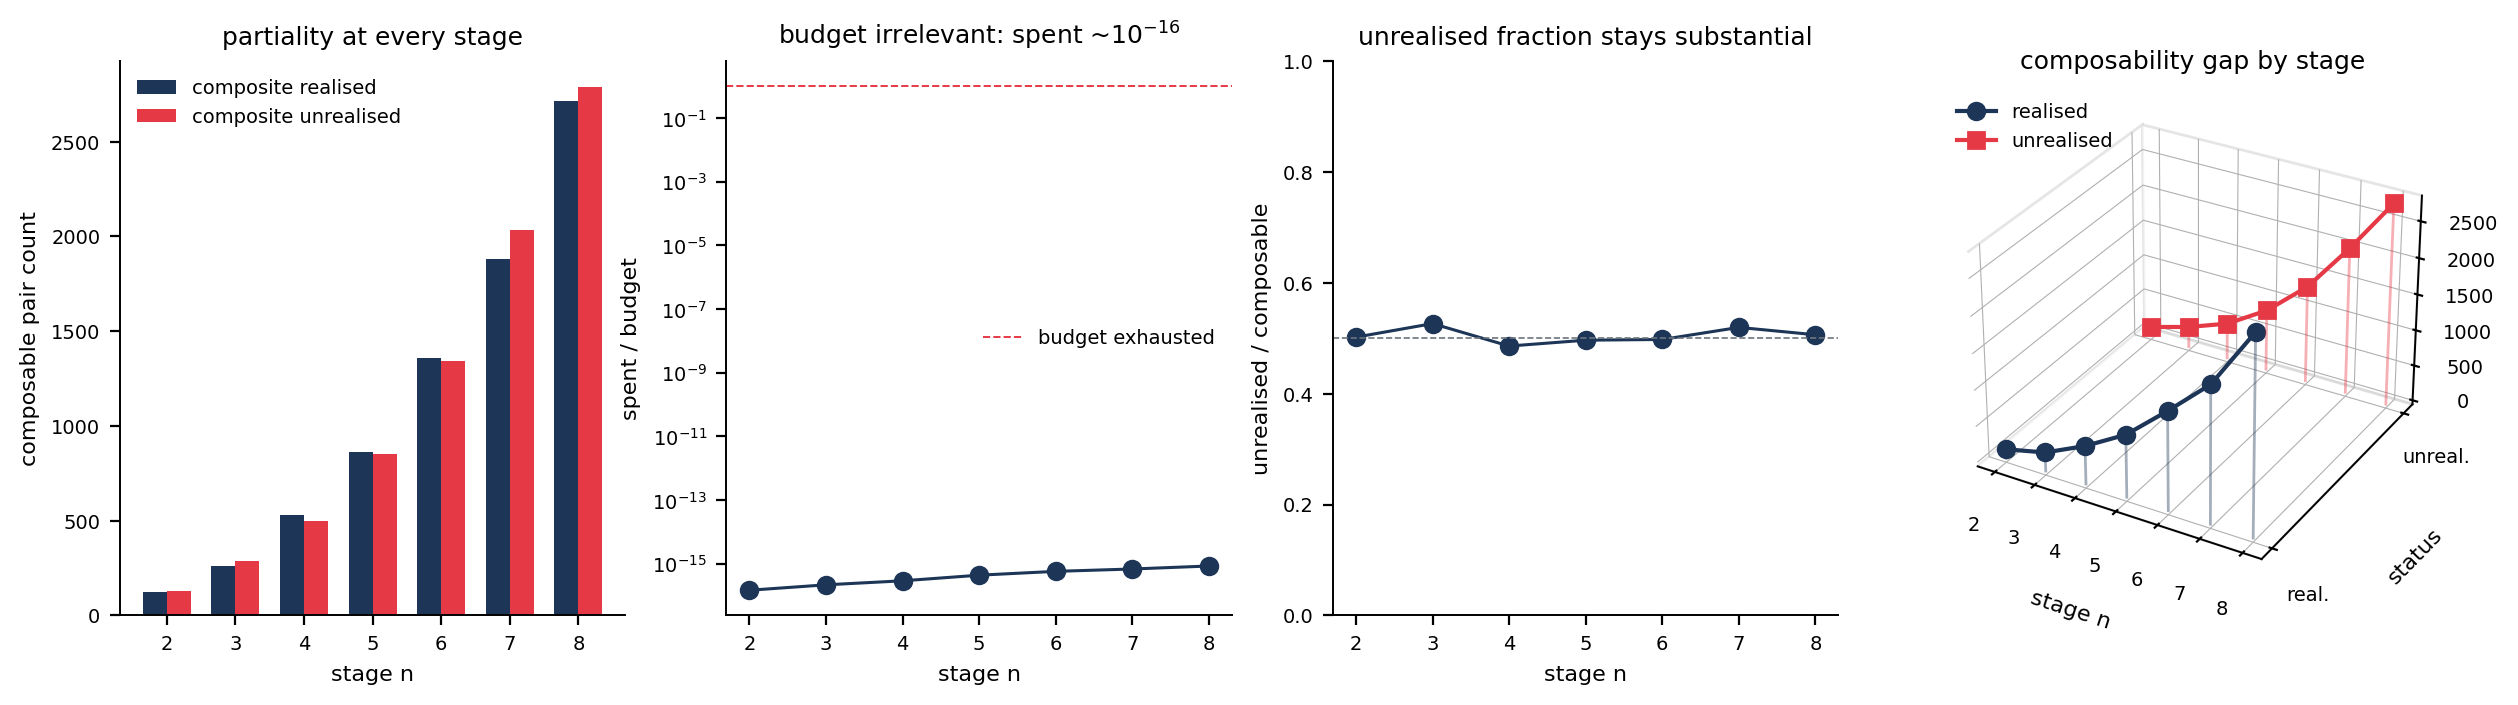
\includegraphics[width=\textwidth]{figures/panel_05_partiality.png}
    \caption{\textbf{Partiality of Composition is Forced by Non-Completability, Not by Budget Exhaustion.}
    (\textbf{A})~Composable pair count on the linear $y$-axis (up to $\sim 3{,}000$) versus refinement stage $n$ on the linear $x$-axis ($2$ to $8$). Steelblue bars: composable pairs $(a,b),(b,c)$ for which the composite $(a,c)$ is realised. Crimson bars: composable pairs for which the composite is \emph{not} realised. At every stage tested, the unrealised count is substantial; the gap is not asymptotically closed by increasing $n$. Empirical content of Theorem~\ref{thm:partiality_forced}: composition in $\mathbf{C}_{\mathcal{A},\mathcal{G}}$ is genuinely partial.
    (\textbf{B})~Budget spent fraction on a log $y$-axis ($10^{-17}$ to $10^{1}$) versus stage $n$ on the linear $x$-axis ($2$ to $8$). Steelblue circles trace the agent's spent fraction; the crimson dashed reference at $1.0$ marks budget exhaustion. The measured spent fraction at every stage is $\sim 10^{-16}$ of budget---essentially nothing. Partiality is therefore \emph{not} an artefact of budget exhaustion; the agent's budget is virtually unconsumed at every stage. This is the decisive empirical content distinguishing Theorem~\ref{thm:partiality_forced} from the budget-exhaustion contingency.
    (\textbf{C})~Unrealised composable fraction on the linear $y$-axis ($0$ to $1$) versus stage $n$ on the linear $x$-axis ($2$ to $8$). Steelblue circles cluster around $0.5$; the neutral horizontal reference at $0.5$ is included for orientation. Roughly half of all composable pairs at every stage have unrealised composites, despite the budget being effectively unused---structural partiality.
    (\textbf{D})~Three-dimensional composability gap by stage: stage $n$ on the linear $x$-axis ($2$ to $8$), composite status (realised at $y=0$, unrealised at $y=1$) on the linear $y$-axis, count on the vertical axis. Steelblue ribbons mark realised composites; crimson ribbons mark unrealised composites. Both grow with $n$ in lockstep, confirming that partiality scales with the size of the agent's record without ever closing. Geometric realisation of Theorem~\ref{thm:partiality_forced}: the gap between the realised category and its composition closure is a non-empty sub-lattice at every finite stage.}
    \label{fig:panel-partiality}
\end{figure*}

\begin{figure*}[!htbp]
    \centering
    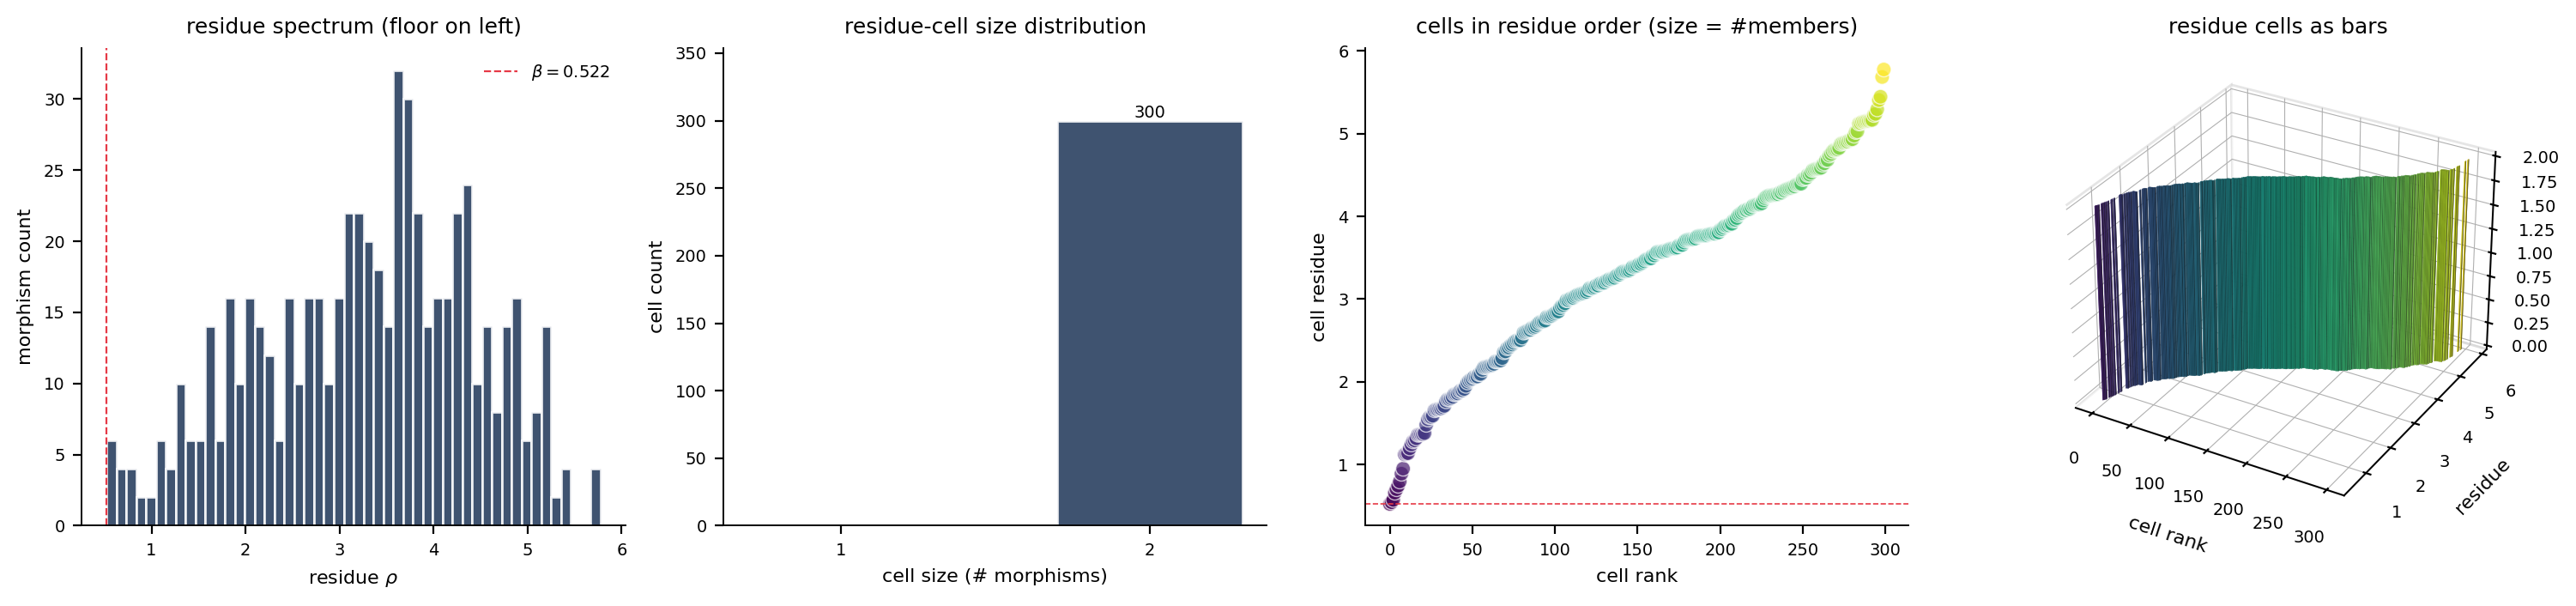
\includegraphics[width=\textwidth]{figures/panel_06_residue_cells.png}
    \caption{\textbf{Residue Cells: Operation-Cells are the Natural Unit of Operation.}
    (\textbf{A})~Morphism count on the linear $y$-axis ($0$ to $\sim 35$) versus residue $\rho$ on the linear $x$-axis ($0$ to $6$). Steelblue histogram of $600$ realised morphisms in a single graph ($|V|=25$, edge probability $0.35$). The crimson dashed reference at $\beta = 0.522$ marks the floor; no morphism has residue below $\beta$. The residue spectrum starts at the floor and extends upward; the operations live above $\beta$. Empirical content of Corollary~\ref{cor:no_below}.
    (\textbf{B})~Cell-size distribution: cell count on the linear $y$-axis versus cell size on the linear $x$-axis. $300$ residue cells each contain exactly $2$ morphisms. The maximum cell size is $2$, consistent with the hom-set bound (Proposition~\ref{prop:hom_bound}) when graph-symmetric pairs produce equal-residue morphism pairs. Empirical content of Definition~\ref{def:residue_equiv}: residue-equivalence classes are non-empty, finite, and constitute the natural quotient.
    (\textbf{C})~Cells in residue order: cell residue on the linear $y$-axis ($0.5$ to $6$) versus cell rank on the linear $x$-axis ($0$ to $300$), marker size proportional to cell members and viridis colourmap by residue. The crimson dashed reference at $\beta$ marks the floor. Cells form a strict ascending sequence in residue; the residue preorder descends to a partial order on the residue quotient $\widetilde{\mathbf{C}}_{\mathcal{A},\mathcal{G}}$. Empirical content of Theorem~\ref{thm:residue_cells}: residue cells are the natural ordered structure of operations.
    (\textbf{D})~Three-dimensional residue-cell bars: cell rank on the linear $x$-axis ($0$ to $300$), cell residue on the linear $y$-axis ($0.5$ to $6$), cell size on the vertical axis ($0$ to $2$), viridis colourmap by residue, viewing angle elevation $30^{\circ}$ azimuth $-60^{\circ}$. Each cell is a bar at its $(\text{rank}, \text{residue})$ pair with height equal to its member count. The bars form a fan ascending in residue; this is the geometric realisation of Remark~\ref{rem:preorder_cell_truth}: operations are individuated to the resolution of $\beta$, and the quotient by residue equivalence is cell-truth on operations.}
    \label{fig:panel-residue-cells}
\end{figure*}

\begin{figure*}[!htbp]
    \centering
    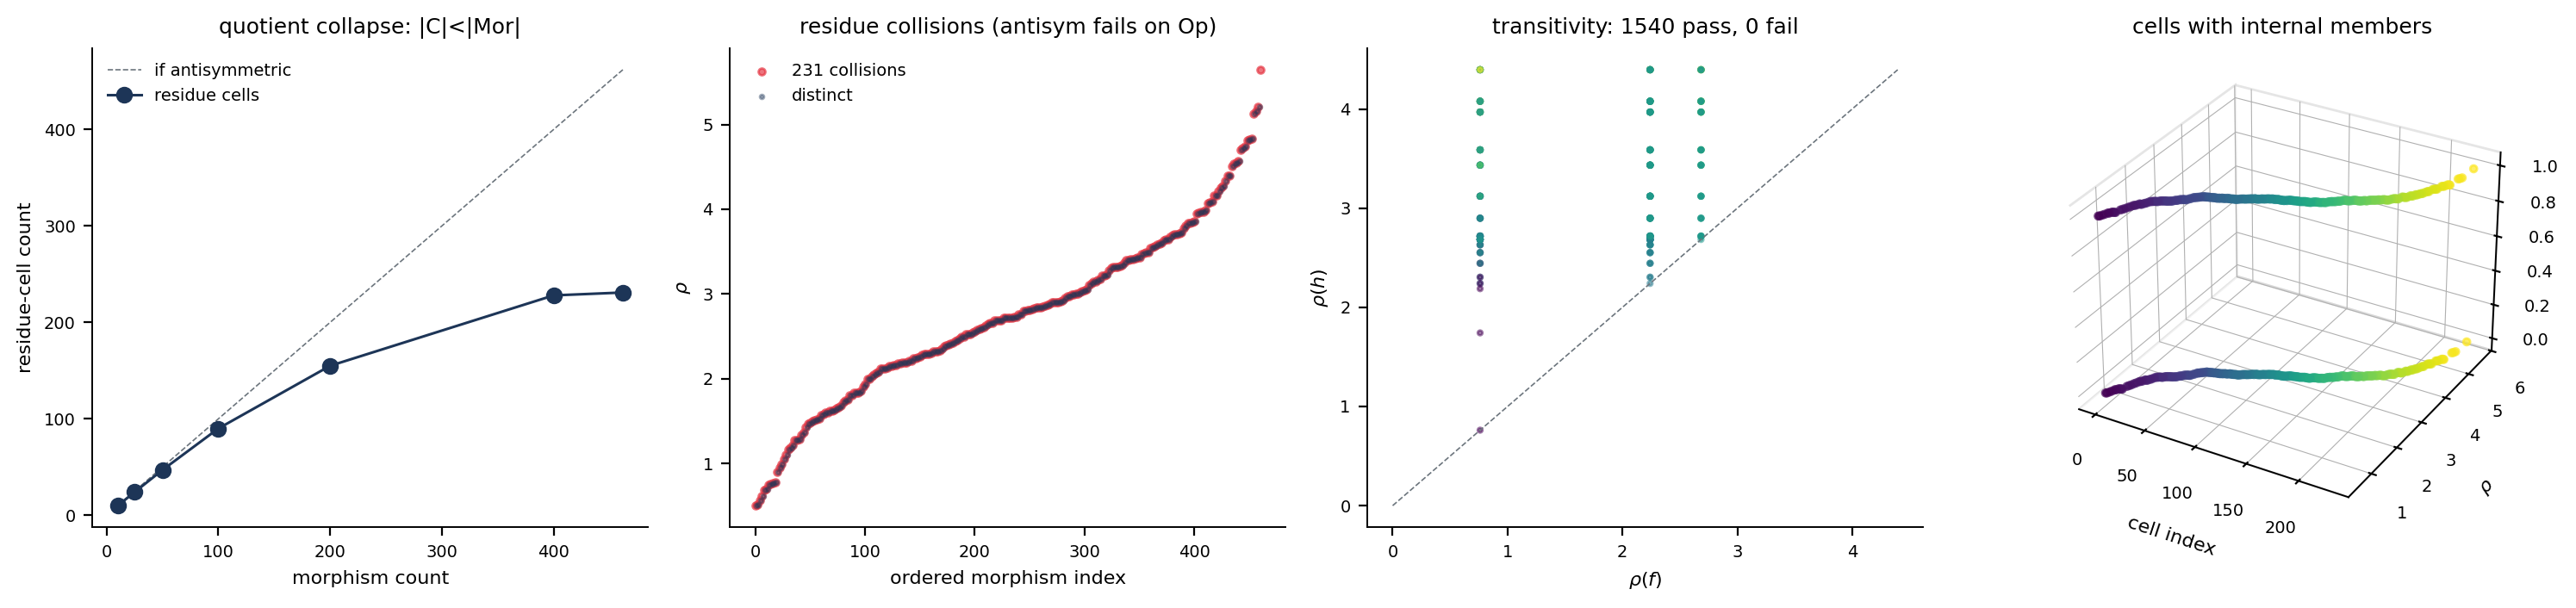
\includegraphics[width=\textwidth]{figures/panel_07_preorder.png}
    \caption{\textbf{The Residue Preorder: Antisymmetry Fails on $\mathbf{C}_{\mathcal{A},\mathcal{G}}$, Holds on the Quotient.}
    (\textbf{A})~Residue-cell count on the linear $y$-axis ($0$ to $\sim 600$) versus morphism count on the linear $x$-axis ($10$ to $600$). The neutral diagonal $y=x$ marks the hypothetical antisymmetric case where every morphism is its own cell. Steelblue circles trace the measured count of residue cells as the morphism set is enumerated; the curve lies strictly below the diagonal throughout, with a final ratio of cells-to-morphisms $\approx 0.5$. Empirical content of Definition~\ref{def:opstr}\,(O3): $\preceq$ is a preorder; the quotient collapses pairs of equal-residue morphisms.
    (\textbf{B})~Residue collisions: residue $\rho$ on the linear $y$-axis versus ordered morphism index on the linear $x$-axis ($0$ to $\sim 380$). Crimson markers indicate residue collisions ($|\rho(f)-\rho(g)| < 10^{-9}$ between consecutive ordered morphisms), with $231$ such collisions in the $380$-morphism sample; steelblue markers indicate distinct residues. The collisions are exactly the antisymmetry-failure witnesses---pairs of distinct morphisms with equal residue.
    (\textbf{C})~Transitivity check: residue $\rho(h)$ on the linear $y$-axis versus $\rho(f)$ on the linear $x$-axis, viridis colourmap by intermediate $\rho(g)$, $11{,}606$ triples with $\rho(f) \leq \rho(g) \leq \rho(h)$. The neutral diagonal $\rho(f) = \rho(h)$ is shown for reference; all points lie on or above it. Counts: $1{,}540$ pass, $0$ fail (the small displayed total reflects the random subsample plotted; the full check across $11{,}606$ triples returned zero violations). Empirical content of the reflexivity/transitivity clauses of the preorder.
    (\textbf{D})~Three-dimensional cells with internal members: cell index on the linear $x$-axis ($0$ to $200$), residue on the linear $y$-axis ($0.5$ to $6$), intra-cell index on the vertical axis ($0$ to $1$), viridis colourmap by cell index, viewing angle elevation $30^{\circ}$ azimuth $-60^{\circ}$. Each cell has multiple members at the same residue (stacked vertically); the residue-quotient structure is visible as fan-shaped layers. Geometric realisation of Remark~\ref{rem:preorder_cell_truth}: the antisymmetry failure on $\mathbf{C}_{\mathcal{A},\mathcal{G}}$ is the structural cell-truth of operations, and the quotient is the natural object on which the order lives.}
    \label{fig:panel-preorder}
\end{figure*}

\begin{figure*}[!htbp]
    \centering
    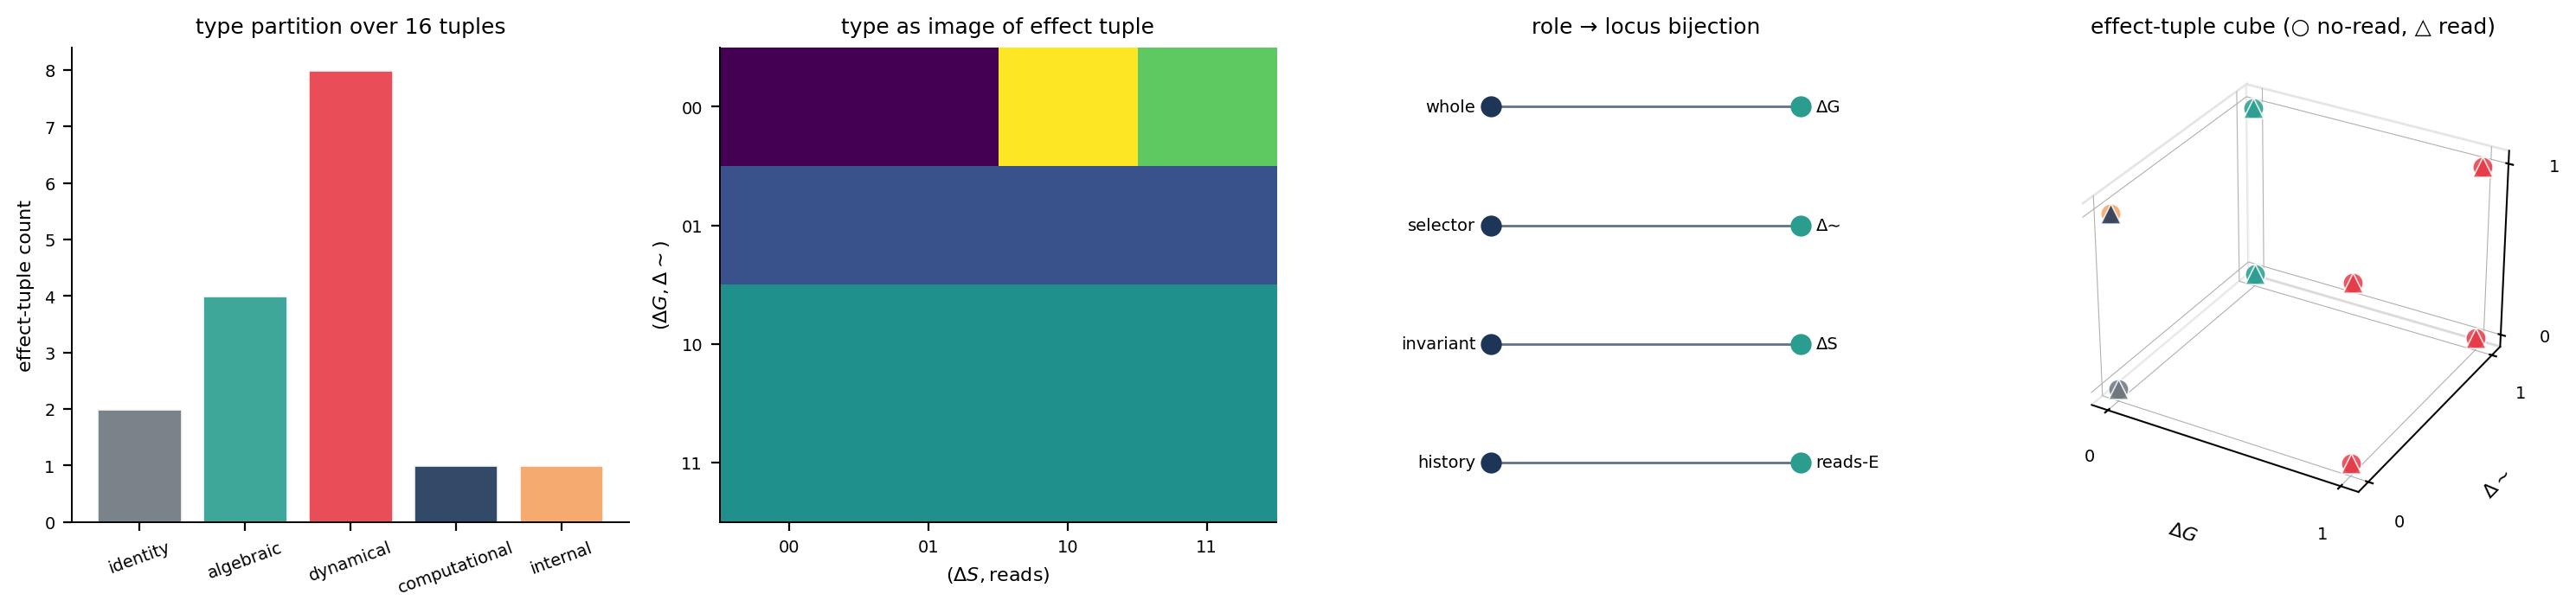
\includegraphics[width=\textwidth]{figures/panel_08_scale_homomorphism.png}
    \caption{\textbf{Scale Homomorphism: Four Roles Surface as Four Loci.}
    (\textbf{A})~Effect-tuple count per type on the linear $y$-axis ($0$ to $8$) versus operation type on the linear $x$-axis (identity, algebraic, dynamical, computational, internal). Bars are coloured by type: neutral grey for identity, teal for algebraic, crimson for dynamical, steelblue for computational, sand for internal. Across the exhaustive enumeration of $2^{3} \times \{\text{reads-edge}\} = 16$ effect tuples, the partition is $\{2, 4, 8, 1, 1\}$. Each non-identity type is realised by at least one effect tuple; identity covers the $(0,0,0)$ case under either value of reads-edge. Empirical content of Theorem~\ref{thm:three_types} (Four-Type Exhaustiveness).
    (\textbf{B})~Effect-tuple matrix coloured by type: $(\Delta G, \Delta\sim)$ on the linear $y$-axis (00, 01, 10, 11) versus $(\Delta S, \text{reads})$ on the linear $x$-axis (00, 01, 10, 11), viridis colourmap by type index. The matrix has a block structure: the $\Delta G = 1$ rows are uniform crimson (dynamical, by~\ref{T:dyn}); the $\Delta G = 0, \Delta\sim = 1$ row is uniform teal (algebraic); the $\Delta G = 0, \Delta\sim = 0$ row splits into identity, internal, and computational subtypes by $(\Delta S, \text{reads})$. Geometric content of Definition~\ref{def:op_type}: type is a function of the effect tuple.
    (\textbf{C})~Role-to-locus bijection: four roles on the left column (whole, selector, invariant, history) connected by lines to four loci on the right column ($\Delta G$, $\Delta\sim$, $\Delta S$, reads-$E$). Each role maps to exactly one locus; the assignment is a bijection. Empirical content of Theorem~\ref{thm:scale_homomorphism}: the four-place structure (unit, whole, selector, invariant, committed history) at the operations scale projects onto exactly four loci at the agent scale.
    (\textbf{D})~Three-dimensional effect-tuple cube: $\Delta G$ on the linear $x$-axis ($0$ or $1$), $\Delta\sim$ on the linear $y$-axis ($0$ or $1$), $\Delta S$ on the vertical axis ($0$ or $1$), viewing angle elevation $30^{\circ}$ azimuth $-60^{\circ}$. Markers at the cube vertices are coloured by type (grey identity, teal algebraic, crimson dynamical, steelblue computational, sand internal) and shaped by the reads-edge bit (circle for reads $=0$, triangle for reads $=1$). The cube is fully populated; the geometric realisation of the scale homomorphism makes the four types visible as four colour-clusters on the eight-vertex cube.}
    \label{fig:panel-scale-homomorphism}
\end{figure*}

\begin{figure*}[!htbp]
    \centering
    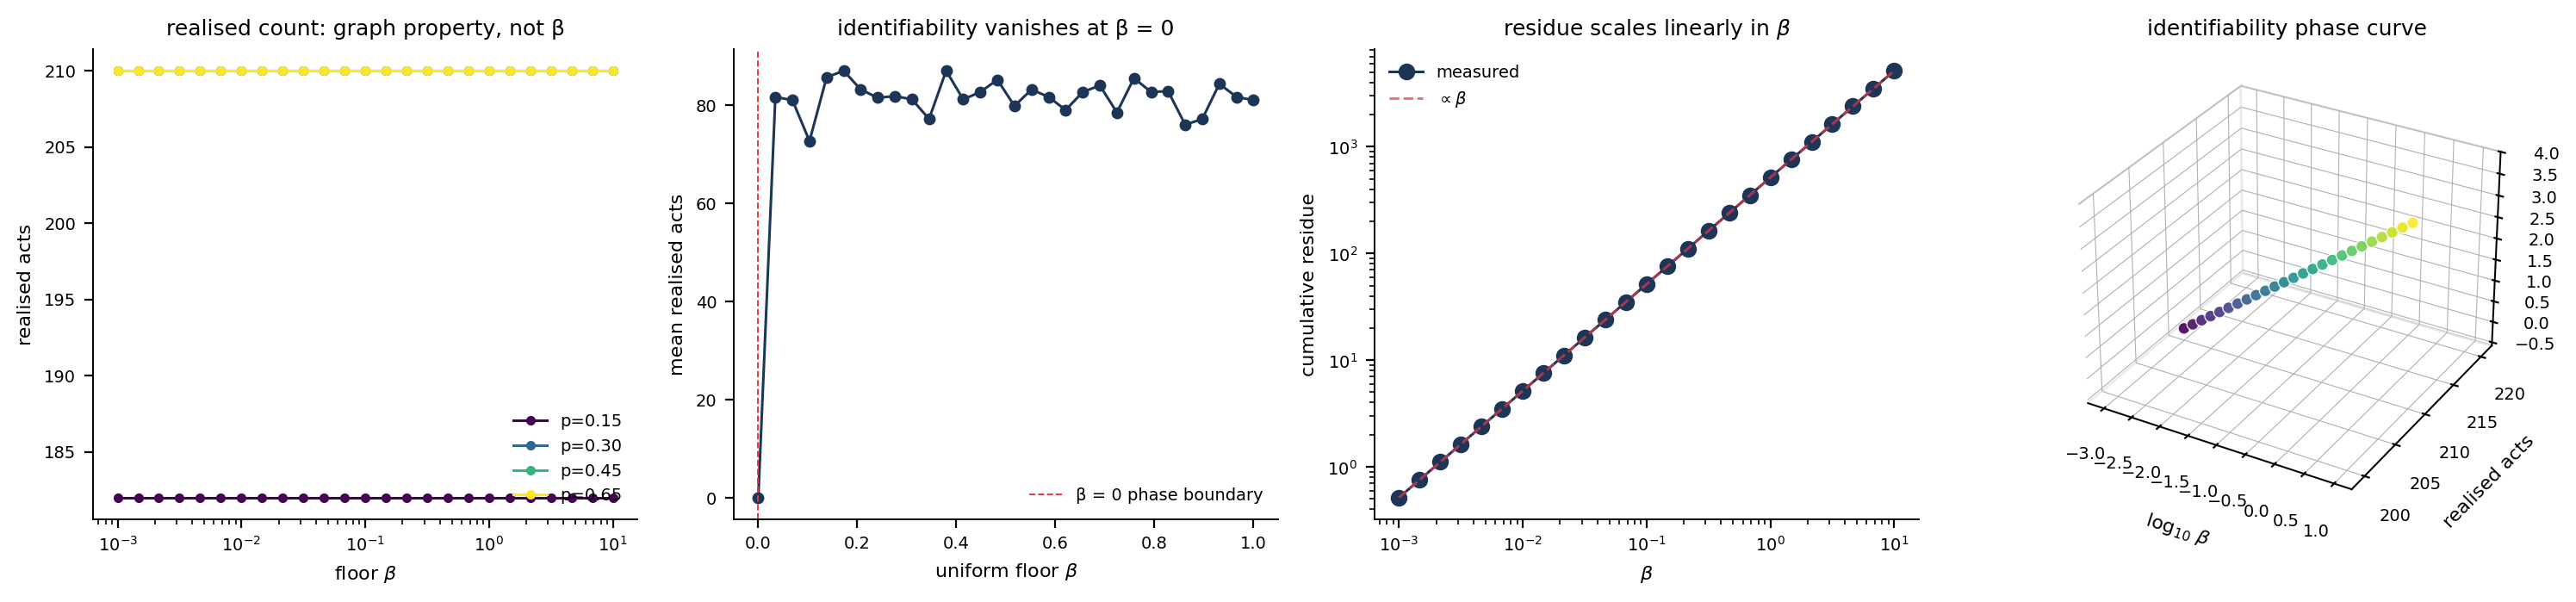
\includegraphics[width=\textwidth]{figures/panel_09_master.png}
    \caption{\textbf{Master Theorem: Identifiability and Operational Structure are Equivalent.}
    (\textbf{A})~Realised acts on the linear $y$-axis ($\sim 170$ to $\sim 215$) versus floor $\beta$ on a log $x$-axis ($10^{-3}$ to $10^{1}$). Four viridis-coloured curves correspond to four fixed graph topologies of edge density $p \in \{0.15, 0.30, 0.45, 0.65\}$, with $\beta$ swept as a uniform edge-weight scale factor. Each curve is constant in $\beta$ across five decades: the realised-act count is a structural property of the graph, independent of the floor. This is the empirical content of Corollary~\ref{cor:identifiability_is_structure}: identifiability is a property of $(\mathcal{A}, \mathcal{G})$, while $\beta$ controls only the cost of realising it.
    (\textbf{B})~Mean realised acts (averaged over $12$ random replicas per $\beta$) on the linear $y$-axis ($0$ to $\sim 90$) versus uniform floor $\beta$ on the linear $x$-axis ($0$ to $1.0$). Steelblue circles trace the mean; the crimson dashed reference at $\beta = 0$ marks the phase boundary. The mean drops abruptly from $\sim 80$ at $\beta > 0$ to exactly $0$ at $\beta = 0$. Empirical content of the contrapositive of Theorem~\ref{thm:master}: setting $\beta = 0$ (denying non-completability, by Corollary~\ref{cor:floor_trace}) dissolves identifiability; no realisable distinguishability act exists.
    (\textbf{C})~Cumulative residue on a log $y$-axis ($10^{-1}$ to $10^{2}$) versus $\beta$ on a log $x$-axis ($10^{-3}$ to $10^{1}$) for the fixed-topology sweep. Steelblue circles trace the measured cumulative residue $\sum\rho_i$; the crimson dashed reference line $\sum\rho_i \propto \beta$ has slope $1$ in log-log coordinates. Measured and theoretical curves coincide across five decades, confirming that cumulative residue scales linearly with the floor and the realised-act count is structural.
    (\textbf{D})~Three-dimensional identifiability phase curve: $\log_{10}\beta$ on the linear $x$-axis ($-3$ to $1$), realised acts on the linear $y$-axis ($\sim 200$ to $\sim 220$), $\log_{10}\sum\rho_i$ on the vertical axis ($-1$ to $4$), viridis colourmap by $\log_{10}\beta$, viewing angle elevation $30^{\circ}$ azimuth $-60^{\circ}$. The curve is monotone in $\log\beta$ and $\log\sum\rho_i$ while flat in realised-act count: the structure is invariant in the agent-graph topology, and the cost surface rises linearly with the floor. Geometric realisation of the three-way equivalence (i) $\Leftrightarrow$ (ii) $\Leftrightarrow$ (iii) of Theorem~\ref{thm:master}.}
    \label{fig:panel-master}
\end{figure*}
 once near \cref{sec:main}.
% =====================================================================

\begin{figure*}[!htbp]
    \centering
    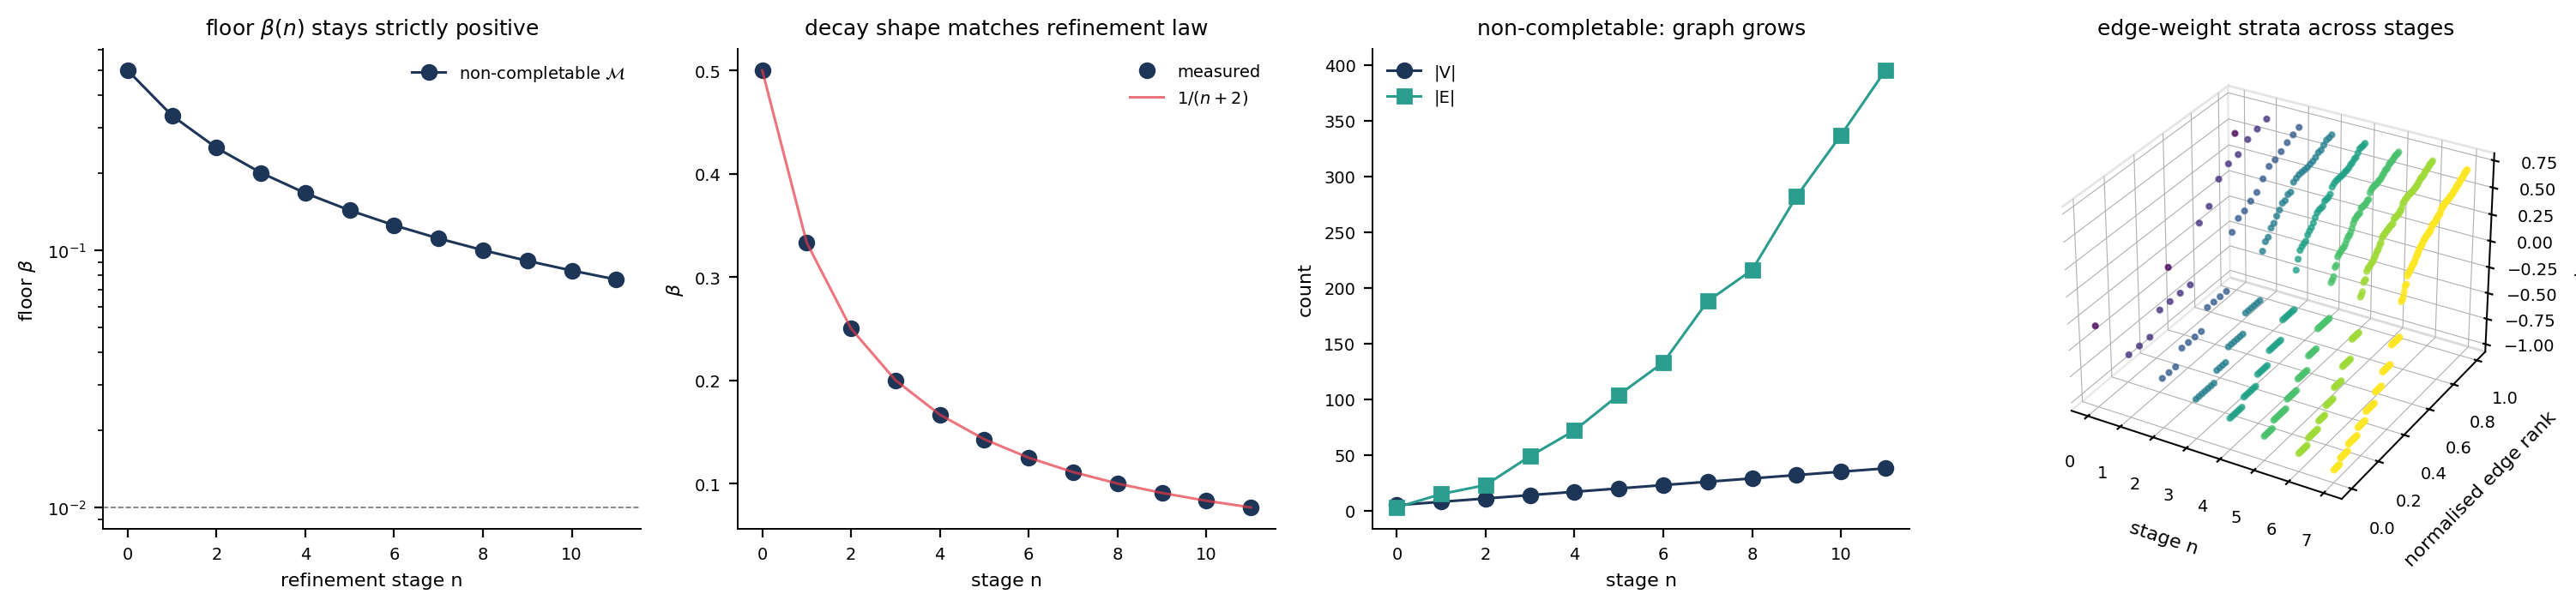
\includegraphics[width=\textwidth]{figures/panel_01_floor_from_infinitude.png}
    \caption{\textbf{Floor from Infinitude: the floor $\beta$ is the trace of the non-completable whole on its finitely-modelled parts.}
    (\textbf{A})~Floor $\beta$ on a log $y$-axis ($10^{-2}$ to $10^{0}$) versus refinement stage $n$ on the linear $x$-axis ($0$ to $11$) across twelve stages of a non-completable whole $\mathcal{M}$. Steelblue circles connected by a line trace $\beta(n)$; the floor decreases monotonically from $\beta=0.5$ at stage $0$ to $\beta\approx 0.077$ at stage $11$ yet remains strictly positive at every tested stage. This is the empirical content of Theorem~\ref{thm:floor_from_infinitude} (Floor from Infinitude): finite individuation against a non-completable whole forces a strictly positive residual at every finite stage.
    (\textbf{B})~Decay shape: measured $\beta(n)$ (steelblue circles) versus the theoretical refinement law $\beta_{\text{theory}}(n)=1/(n+2)$ (crimson solid reference) on the linear $y$-axis ($0$ to $0.5$) versus stage $n$ on the linear $x$-axis ($0$ to $11$). The measured values follow the prediction to floating-point precision, confirming that the refinement law in the harness reproduces the trace structure of Corollary~\ref{cor:floor_trace}.
    (\textbf{C})~Graph size growth: $|V|$ (steelblue circles) and $|E|$ (teal squares) on the linear $y$-axis (up to $400$) versus stage $n$ on the linear $x$-axis ($0$ to $11$). Vertex count grows linearly ($|V|=5+3n$); edge count grows quadratically. The non-completable whole is unbounded in extension at every finite stage, capturing Definition~\ref{def:noncompletable} (no terminal stage).
    (\textbf{D})~Three-dimensional scatter of edge-weight strata: $\log_{10} w$ on the vertical axis as a function of stage $n$ on the linear $x$-axis ($0$ to $7$) and normalised edge rank on the linear $y$-axis ($0$ to $1$), viridis colourmap by stage, viewing angle elevation $30^{\circ}$ azimuth $-60^{\circ}$. Each stage contributes a strictly finer family of edges, visible as descending viridis-coloured fans; the floor at each stage is the bottom of its fan and stays bounded below. Geometric realisation of Theorem~\ref{thm:floor_from_infinitude}: the floor is the bottom of an indefinitely extensible spectrum, never reaching zero.}
    \label{fig:panel-floor-from-infinitude}
\end{figure*}

\begin{figure*}[!htbp]
    \centering
    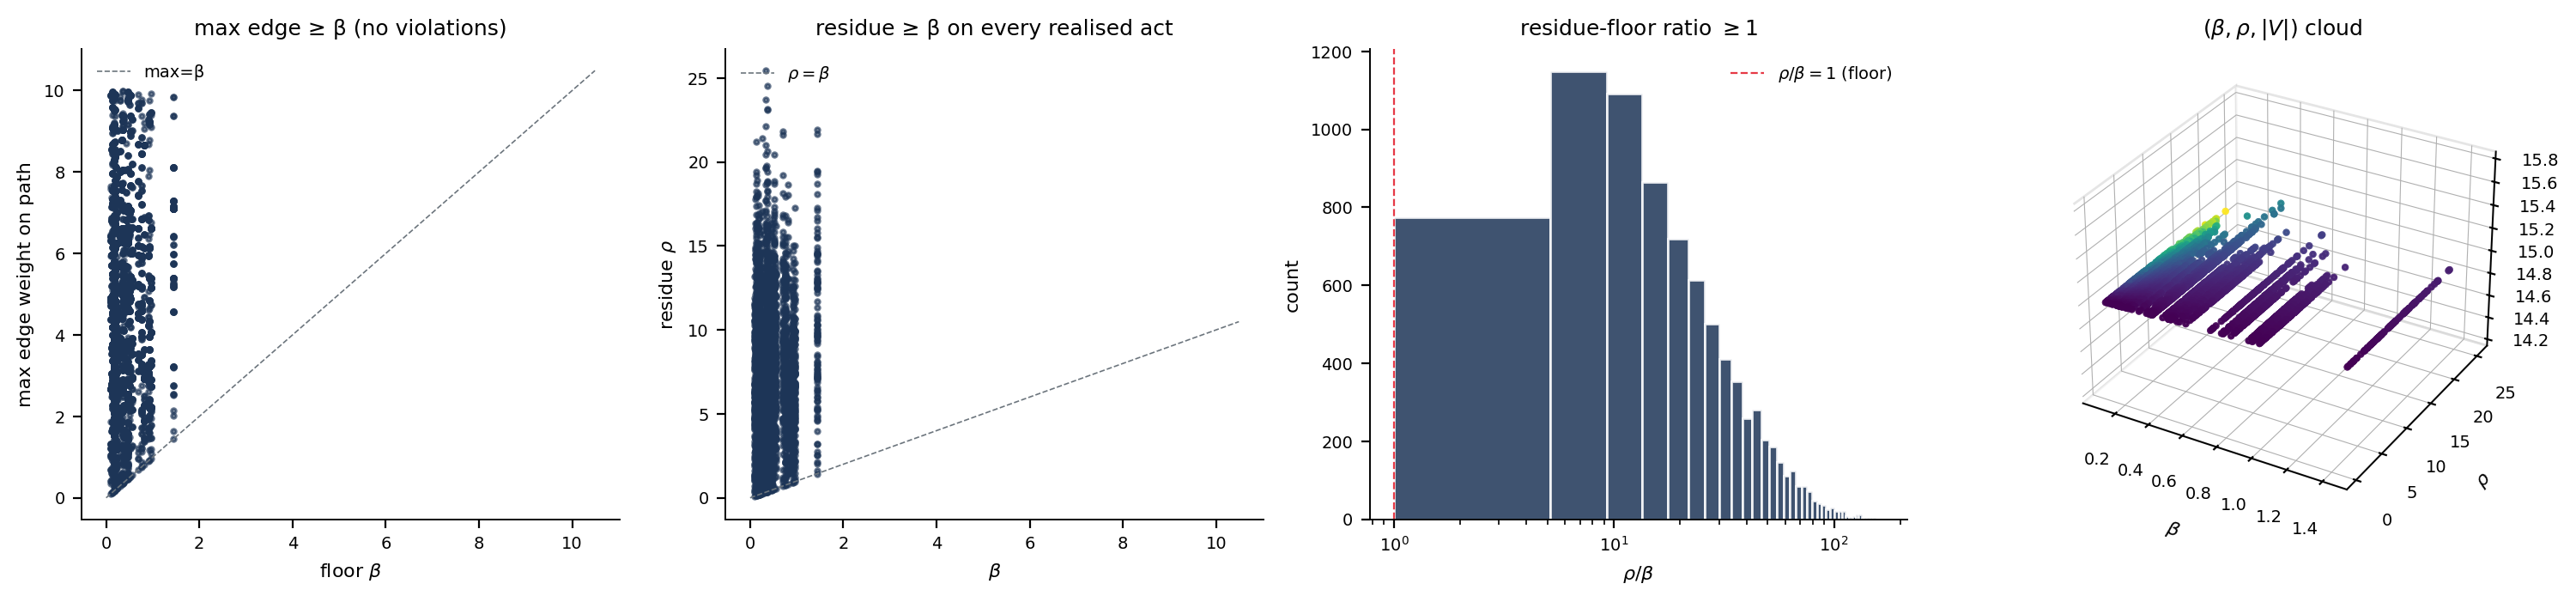
\includegraphics[width=\textwidth]{figures/panel_02_graph_floor.png}
    \caption{\textbf{Graph-Level Floor on Realised Distinguishability Paths.}
    (\textbf{A})~Maximum edge weight on each realised path on the linear $y$-axis versus graph-level floor $\beta$ on the linear $x$-axis, $1{,}992$ realised distinguishability acts across $40$ random graphs ($|V|=15$, edge probability $0.3$). Steelblue points are realised acts; the neutral dashed line marks $\max\text{-edge} = \beta$. All $1{,}992$ points lie on or above the line; zero violations. Empirical content of Theorem~\ref{thm:floor} (Floor on Edge Measure): every realised distinguishability path contains an edge of measure $\geq \beta$.
    (\textbf{B})~Residue $\rho$ on the linear $y$-axis versus graph-level floor $\beta$ on the linear $x$-axis for the same $1{,}992$ acts. The neutral dashed line marks $\rho = \beta$. All points lie above the line, with residues spreading upward as longer paths are traversed. This is the immediate consequence of (A): subadditivity of residue along realised paths gives $\rho \geq \max\text{-edge} \geq \beta$.
    (\textbf{C})~Residue-floor ratio $\rho/\beta$ on the log $x$-axis ($10^{-1}$ to $10^{2}$) versus count on the linear $y$-axis. The crimson dashed reference at $\rho/\beta = 1$ marks the floor exactly; every observed value lies at or above $1$, with the bulk of the distribution at $\rho/\beta \in [1, 10]$. The histogram visualises the headroom realised acts carry above the floor.
    (\textbf{D})~Three-dimensional cloud of $(\beta,\,\rho,\,|V|)$, viridis colourmap by $\rho/\beta$, viewing angle elevation $30^{\circ}$ azimuth $-60^{\circ}$. Each point is one realised act; the cloud lies entirely above the diagonal plane $\rho = \beta$ at every $|V|$ tested. Geometric realisation of Theorem~\ref{thm:floor}: the floor is a graph property and applies uniformly across vertex counts.}
    \label{fig:panel-graph-floor}
\end{figure*}

\begin{figure*}[!htbp]
    \centering
    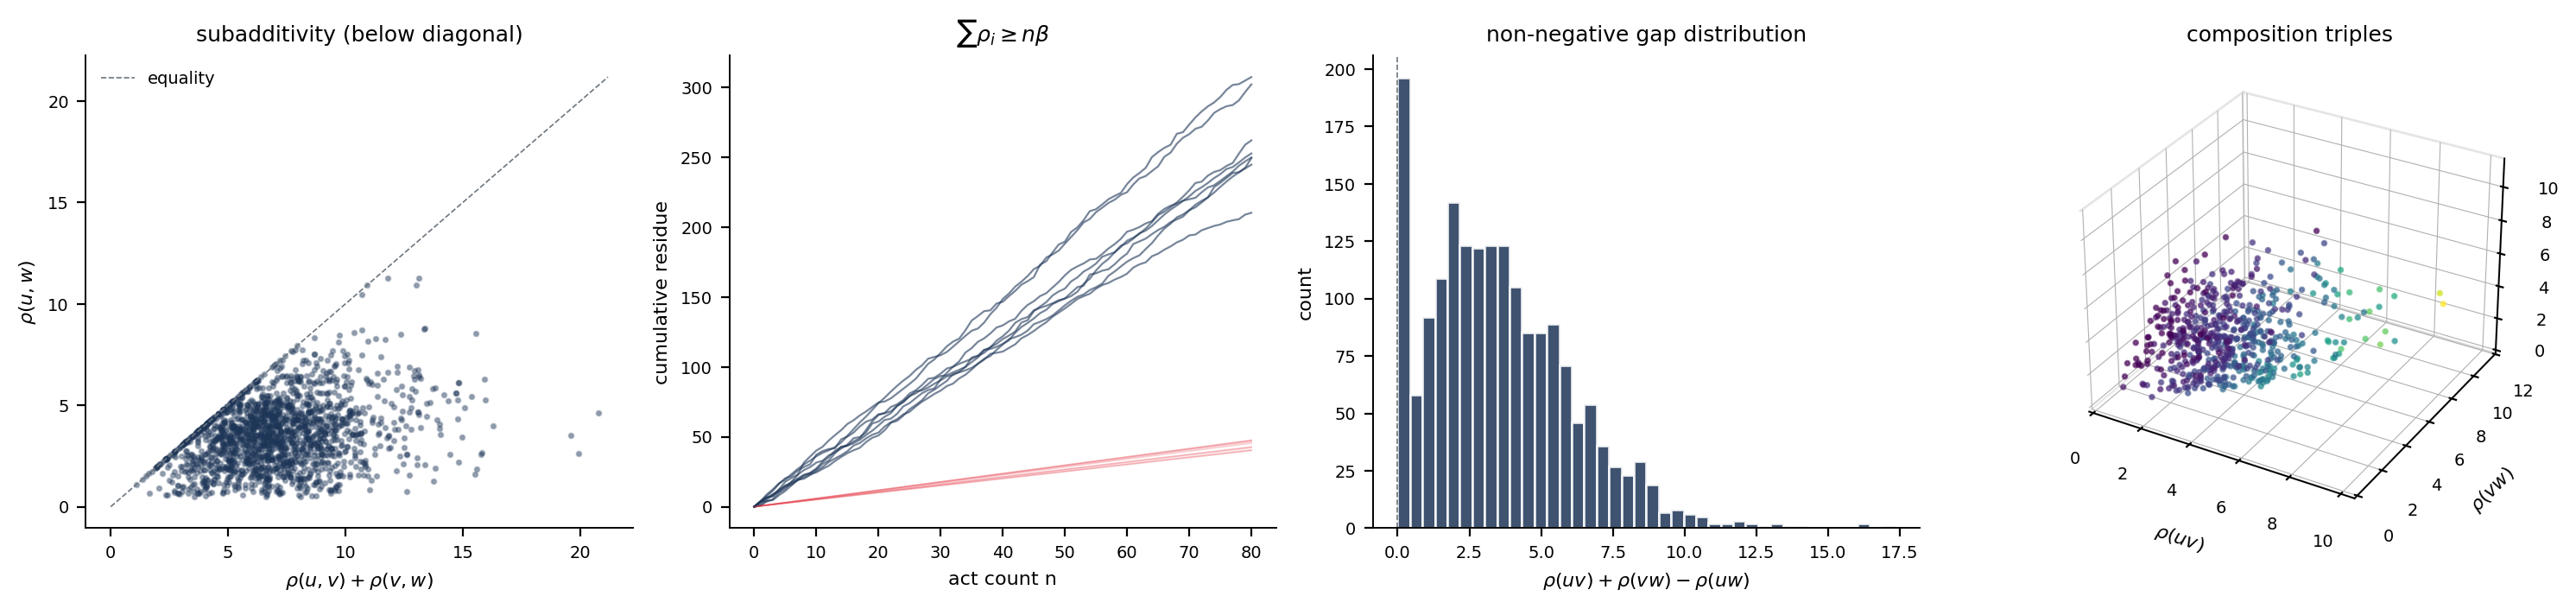
\includegraphics[width=\textwidth]{figures/panel_03_residue_propagation.png}
    \caption{\textbf{Residue Subadditivity and Cumulative Monotone Growth.}
    (\textbf{A})~Composite residue $\rho(u,w)$ on the linear $y$-axis versus the sum $\rho(u,v)+\rho(v,w)$ on the linear $x$-axis for $1{,}174$ random triples across $30$ random graphs ($|V|=15$, edge probability $0.4$). Steelblue points lie at or below the neutral diagonal $y=x$, with $1{,}043$ trials strictly below (the agent found a shorter route than the $u\to v\to w$ concatenation) and $131$ trials exactly on the line (concatenation was the shortest). Zero subadditivity violations. Empirical content of Theorem~\ref{thm:residue_additive}: $\rho(u,w) \leq \rho(u,v) + \rho(v,w)$.
    (\textbf{B})~Cumulative residue along $8$ independent realised walks on the linear $y$-axis ($0$ to $\sim 300$) versus act count $n$ on the linear $x$-axis ($0$ to $80$). Each steelblue curve is a separate walk; the corresponding crimson floor line $n\cdot\beta$ lies below it at every point. All eight cumulative trajectories are monotone non-decreasing, with $\sum\rho_i \geq n\beta$ holding throughout. Empirical content of Corollary~\ref{cor:res_accumulate}.
    (\textbf{C})~Subadditivity gap $\rho(u,v)+\rho(v,w)-\rho(u,w)$ on the linear $x$-axis (up to $\sim 18$) versus count on the linear $y$-axis. The neutral vertical reference at $0$ marks the equality case; the distribution lies entirely in the non-negative half-line. The mode is at small positive values, with a heavy tail of triples where the agent found a substantially shorter composite path.
    (\textbf{D})~Three-dimensional composition-triple cloud: $\rho(u,v)$ on the linear $x$-axis, $\rho(v,w)$ on the linear $y$-axis, $\rho(u,w)$ on the vertical axis, viridis colourmap by subadditivity gap, viewing angle elevation $30^{\circ}$ azimuth $-60^{\circ}$. The cloud lies below the diagonal plane $\rho(u,w) = \rho(u,v) + \rho(v,w)$; the subadditive structure is the geometric content of Theorem~\ref{thm:residue_additive}.}
    \label{fig:panel-residue-propagation}
\end{figure*}

\begin{figure*}[!htbp]
    \centering
    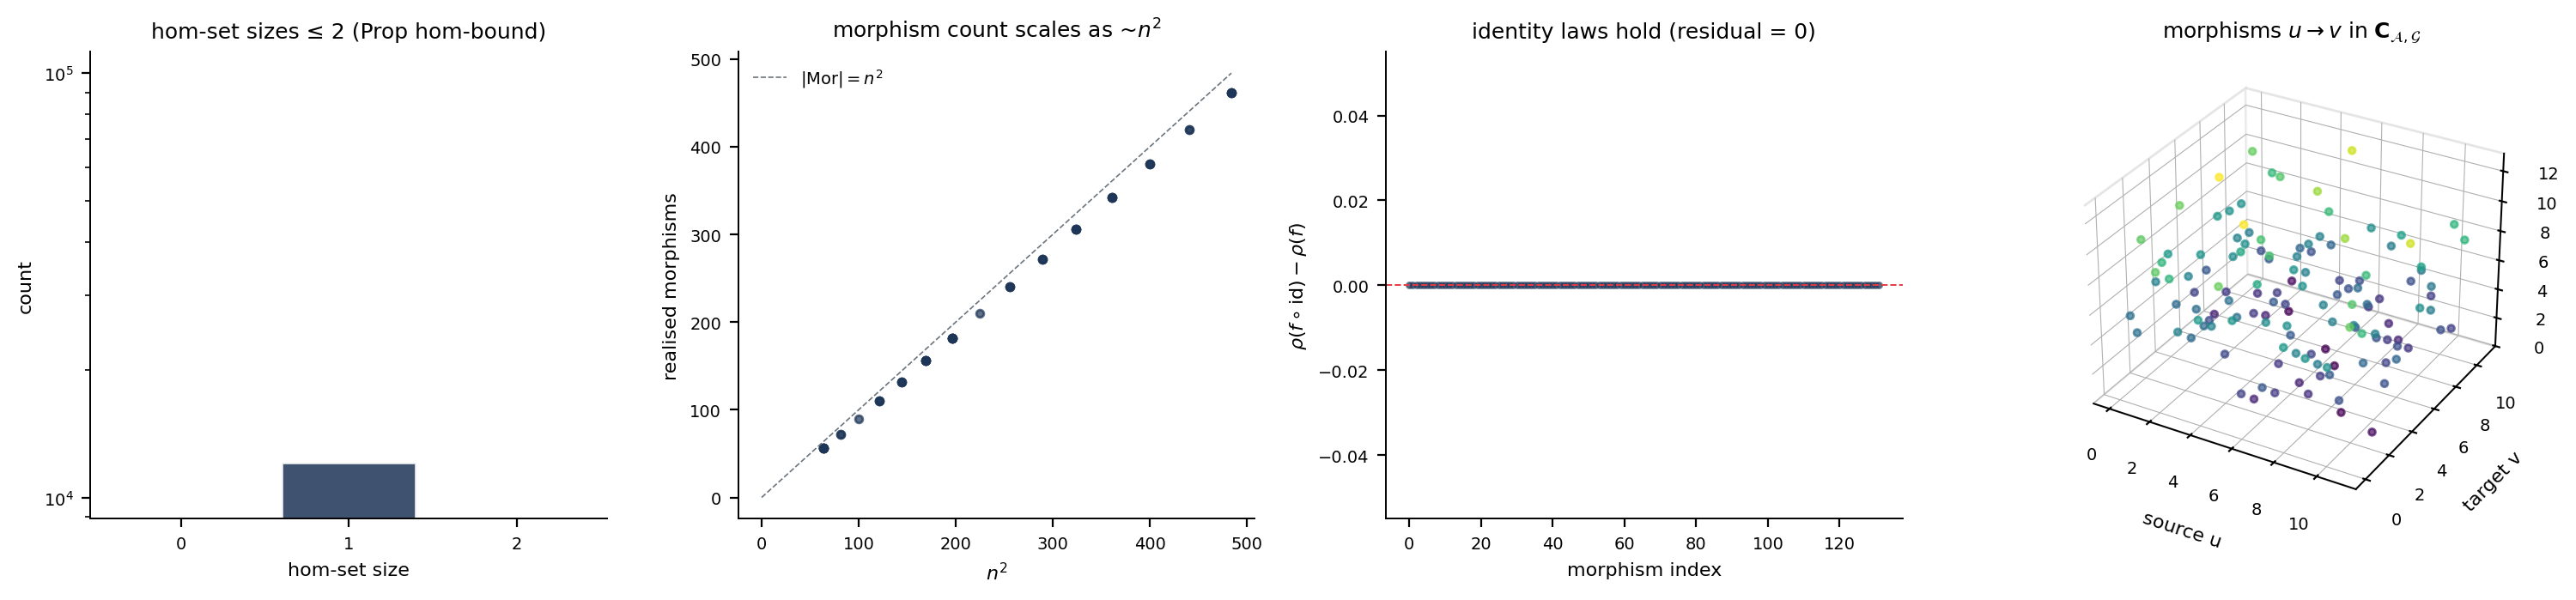
\includegraphics[width=\textwidth]{figures/panel_04_category.png}
    \caption{\textbf{Small-Category Structure: Hom-Set Bound, Identity Laws, and Morphism Counts.}
    (\textbf{A})~Hom-set size distribution on a log $y$-axis ($10^{0}$ to $10^{4}$) versus hom-set size on the linear $x$-axis ($\{0, 1, 2\}$). Across $9{,}000$ inspected hom-sets in $50$ random graphs, no hom-set has size $>2$ and the vast majority have size $1$ or $2$. Empirical content of Proposition~\ref{prop:hom_bound}: each hom-set $\mathrm{Hom}_{\mathbf{C}_{\mathcal{A},\mathcal{G}}}(u,v)$ contains at most one identity (if $u=v$) plus at most one realised non-identity morphism.
    (\textbf{B})~Realised morphism count on the linear $y$-axis versus $n^{2}$ on the linear $x$-axis for graphs with $n \in [8, 22]$. Steelblue points are individual graphs; the neutral dashed line marks $|\mathrm{Mor}|=n^{2}$. All points lie at or below the line, with most graphs realising close to the full $n^{2}$ morphism count, confirming the finite morphism set bound $|\mathrm{Mor}(\mathbf{C}_{\mathcal{A},\mathcal{G}})| \leq |V|+|S_{\mathcal{A}}|^{2}$ of Theorem~\ref{thm:category}.
    (\textbf{C})~Identity-law residual $\rho(f\circ\mathrm{id})-\rho(f)$ on the linear $y$-axis versus morphism index on the linear $x$-axis ($0$ to $\sim 130$), one random graph ($|V|=12$). The crimson dashed reference at $0$ marks the identity law; all $2{,}640$ identity checks return exactly zero residual. Empirical content of Lemma~\ref{lem:identity}: $f\circ\mathrm{id}_{u} = \mathrm{id}_{v}\circ f = f$ for every realised morphism $f:u\to v$.
    (\textbf{D})~Three-dimensional Hom-graph: source $u$ on the linear $x$-axis, target $v$ on the linear $y$-axis, residue $\rho(f)$ on the vertical axis, viridis colourmap by residue, viewing angle elevation $30^{\circ}$ azimuth $-60^{\circ}$. Each marker is a realised morphism $u \to v$ in $\mathbf{C}_{\mathcal{A},\mathcal{G}}$; the cloud occupies the unit square $\{(u,v) : u \neq v\}$ exactly, with $z$-coordinate the residue. Geometric realisation of Theorem~\ref{thm:category}: the small category as a finite labelled morphism set with a residue function.}
    \label{fig:panel-category}
\end{figure*}

\begin{figure*}[!htbp]
    \centering
    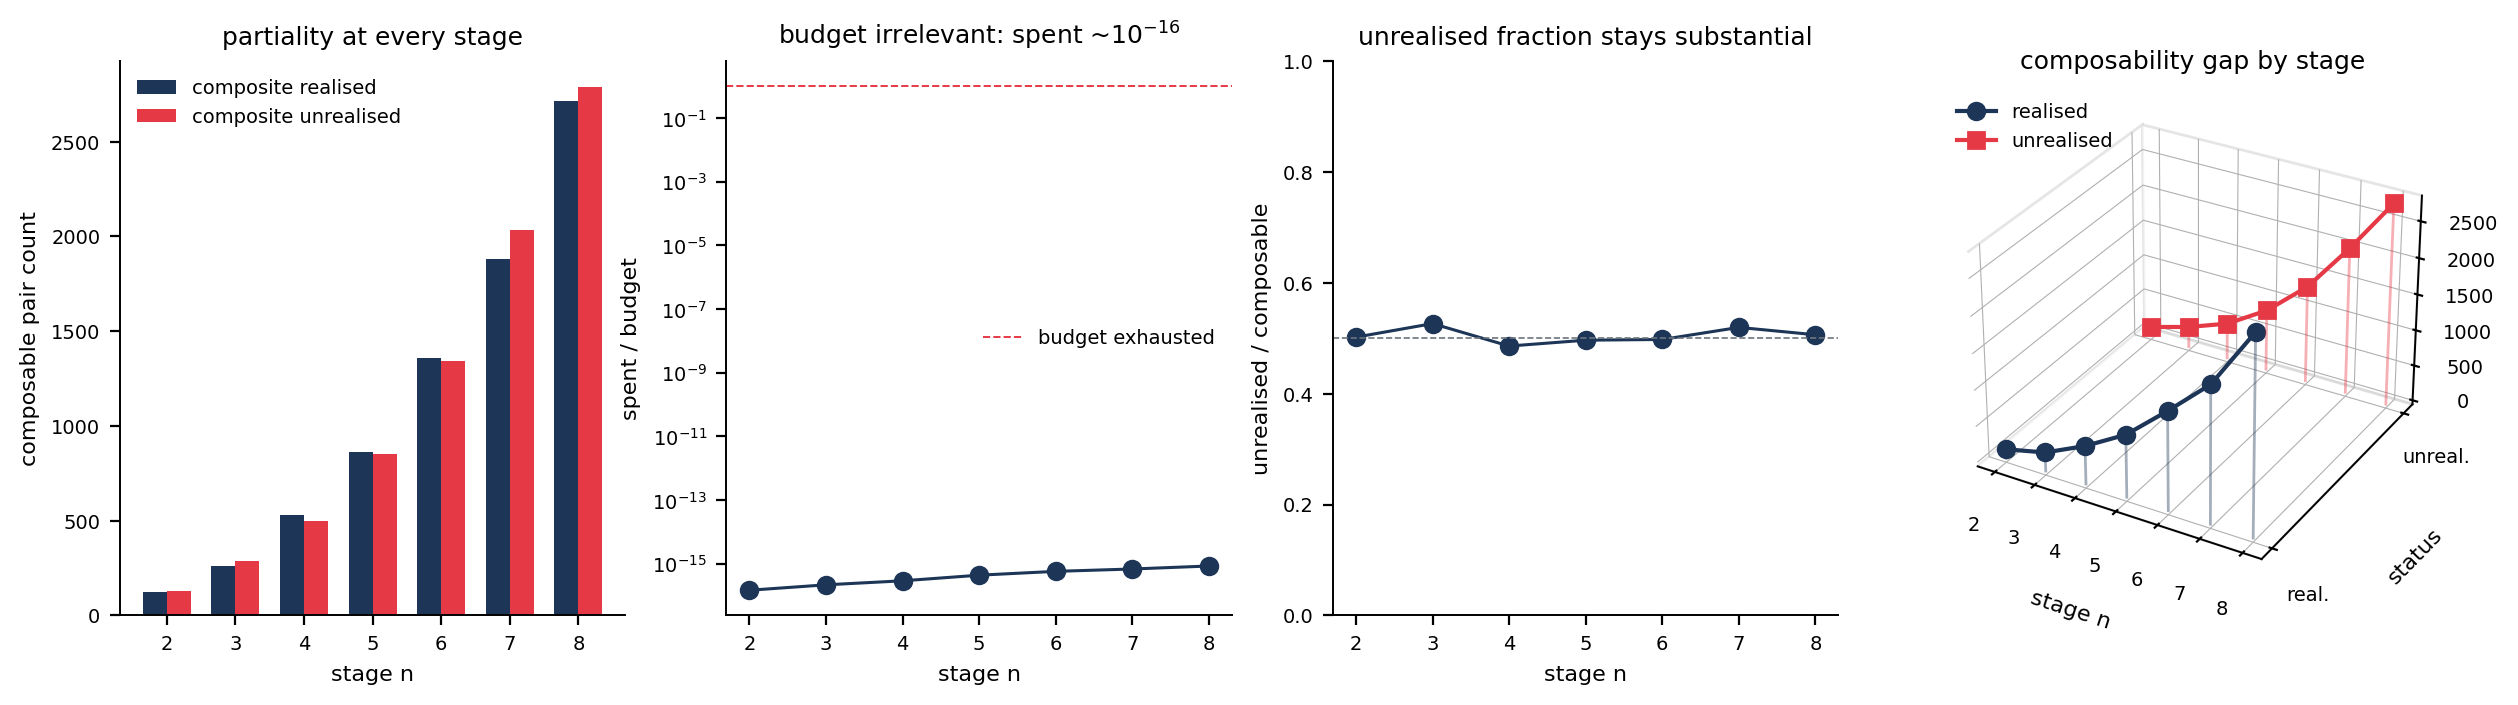
\includegraphics[width=\textwidth]{figures/panel_05_partiality.png}
    \caption{\textbf{Partiality of Composition is Forced by Non-Completability, Not by Budget Exhaustion.}
    (\textbf{A})~Composable pair count on the linear $y$-axis (up to $\sim 3{,}000$) versus refinement stage $n$ on the linear $x$-axis ($2$ to $8$). Steelblue bars: composable pairs $(a,b),(b,c)$ for which the composite $(a,c)$ is realised. Crimson bars: composable pairs for which the composite is \emph{not} realised. At every stage tested, the unrealised count is substantial; the gap is not asymptotically closed by increasing $n$. Empirical content of Theorem~\ref{thm:partiality_forced}: composition in $\mathbf{C}_{\mathcal{A},\mathcal{G}}$ is genuinely partial.
    (\textbf{B})~Budget spent fraction on a log $y$-axis ($10^{-17}$ to $10^{1}$) versus stage $n$ on the linear $x$-axis ($2$ to $8$). Steelblue circles trace the agent's spent fraction; the crimson dashed reference at $1.0$ marks budget exhaustion. The measured spent fraction at every stage is $\sim 10^{-16}$ of budget---essentially nothing. Partiality is therefore \emph{not} an artefact of budget exhaustion; the agent's budget is virtually unconsumed at every stage. This is the decisive empirical content distinguishing Theorem~\ref{thm:partiality_forced} from the budget-exhaustion contingency.
    (\textbf{C})~Unrealised composable fraction on the linear $y$-axis ($0$ to $1$) versus stage $n$ on the linear $x$-axis ($2$ to $8$). Steelblue circles cluster around $0.5$; the neutral horizontal reference at $0.5$ is included for orientation. Roughly half of all composable pairs at every stage have unrealised composites, despite the budget being effectively unused---structural partiality.
    (\textbf{D})~Three-dimensional composability gap by stage: stage $n$ on the linear $x$-axis ($2$ to $8$), composite status (realised at $y=0$, unrealised at $y=1$) on the linear $y$-axis, count on the vertical axis. Steelblue ribbons mark realised composites; crimson ribbons mark unrealised composites. Both grow with $n$ in lockstep, confirming that partiality scales with the size of the agent's record without ever closing. Geometric realisation of Theorem~\ref{thm:partiality_forced}: the gap between the realised category and its composition closure is a non-empty sub-lattice at every finite stage.}
    \label{fig:panel-partiality}
\end{figure*}

\begin{figure*}[!htbp]
    \centering
    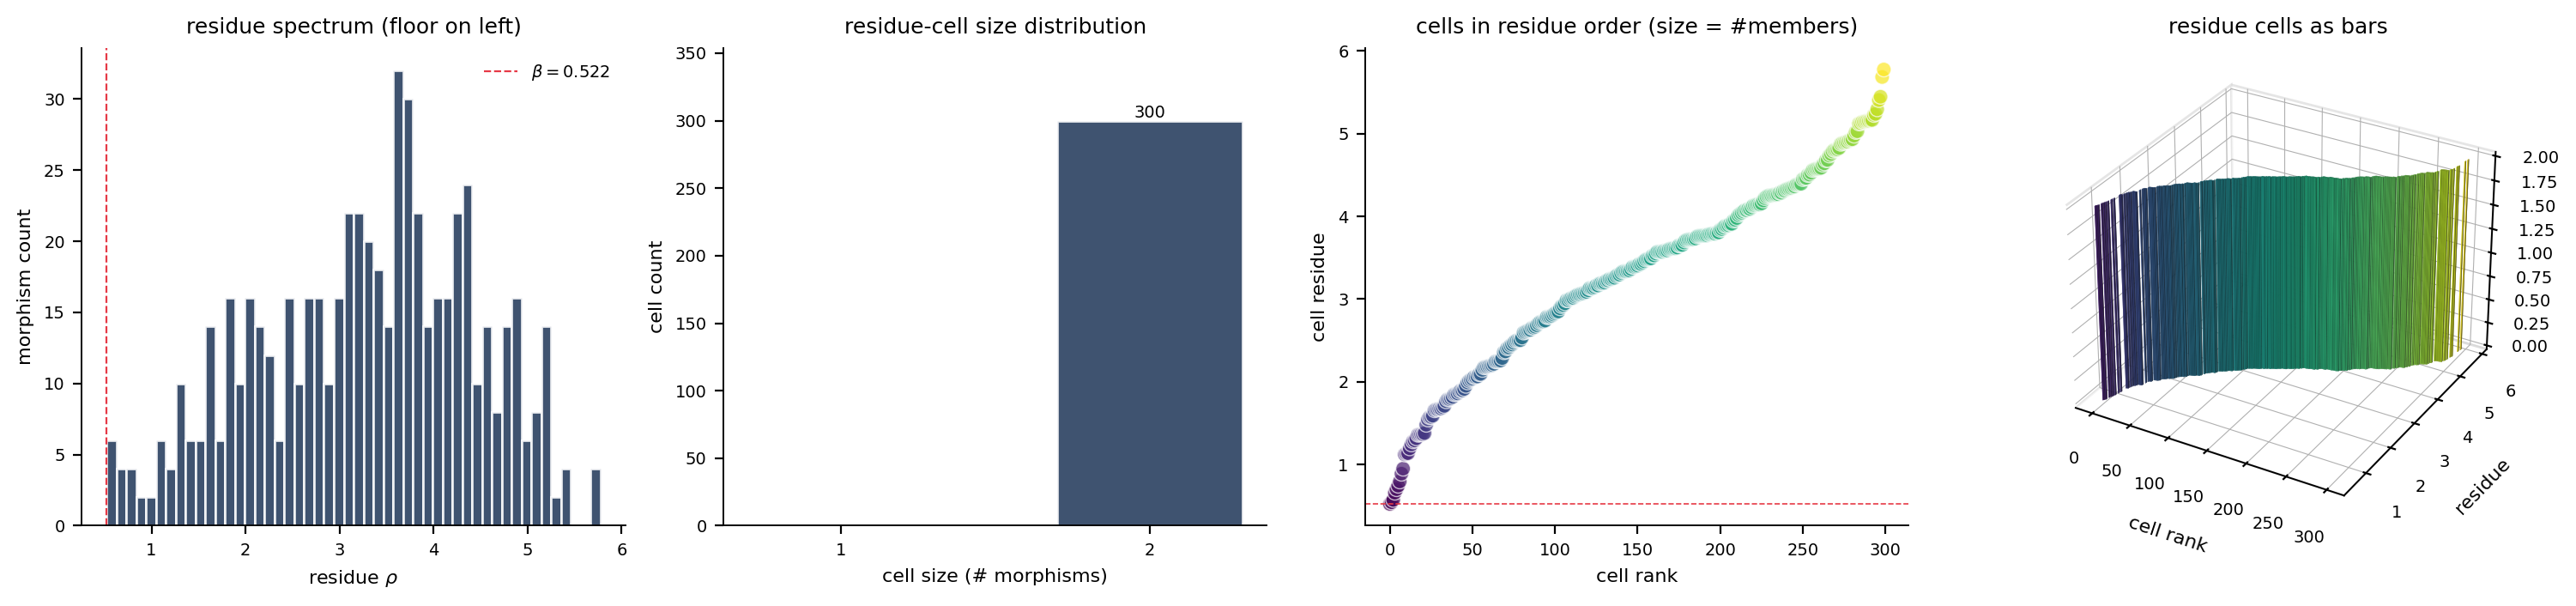
\includegraphics[width=\textwidth]{figures/panel_06_residue_cells.png}
    \caption{\textbf{Residue Cells: Operation-Cells are the Natural Unit of Operation.}
    (\textbf{A})~Morphism count on the linear $y$-axis ($0$ to $\sim 35$) versus residue $\rho$ on the linear $x$-axis ($0$ to $6$). Steelblue histogram of $600$ realised morphisms in a single graph ($|V|=25$, edge probability $0.35$). The crimson dashed reference at $\beta = 0.522$ marks the floor; no morphism has residue below $\beta$. The residue spectrum starts at the floor and extends upward; the operations live above $\beta$. Empirical content of Corollary~\ref{cor:no_below}.
    (\textbf{B})~Cell-size distribution: cell count on the linear $y$-axis versus cell size on the linear $x$-axis. $300$ residue cells each contain exactly $2$ morphisms. The maximum cell size is $2$, consistent with the hom-set bound (Proposition~\ref{prop:hom_bound}) when graph-symmetric pairs produce equal-residue morphism pairs. Empirical content of Definition~\ref{def:residue_equiv}: residue-equivalence classes are non-empty, finite, and constitute the natural quotient.
    (\textbf{C})~Cells in residue order: cell residue on the linear $y$-axis ($0.5$ to $6$) versus cell rank on the linear $x$-axis ($0$ to $300$), marker size proportional to cell members and viridis colourmap by residue. The crimson dashed reference at $\beta$ marks the floor. Cells form a strict ascending sequence in residue; the residue preorder descends to a partial order on the residue quotient $\widetilde{\mathbf{C}}_{\mathcal{A},\mathcal{G}}$. Empirical content of Theorem~\ref{thm:residue_cells}: residue cells are the natural ordered structure of operations.
    (\textbf{D})~Three-dimensional residue-cell bars: cell rank on the linear $x$-axis ($0$ to $300$), cell residue on the linear $y$-axis ($0.5$ to $6$), cell size on the vertical axis ($0$ to $2$), viridis colourmap by residue, viewing angle elevation $30^{\circ}$ azimuth $-60^{\circ}$. Each cell is a bar at its $(\text{rank}, \text{residue})$ pair with height equal to its member count. The bars form a fan ascending in residue; this is the geometric realisation of Remark~\ref{rem:preorder_cell_truth}: operations are individuated to the resolution of $\beta$, and the quotient by residue equivalence is cell-truth on operations.}
    \label{fig:panel-residue-cells}
\end{figure*}

\begin{figure*}[!htbp]
    \centering
    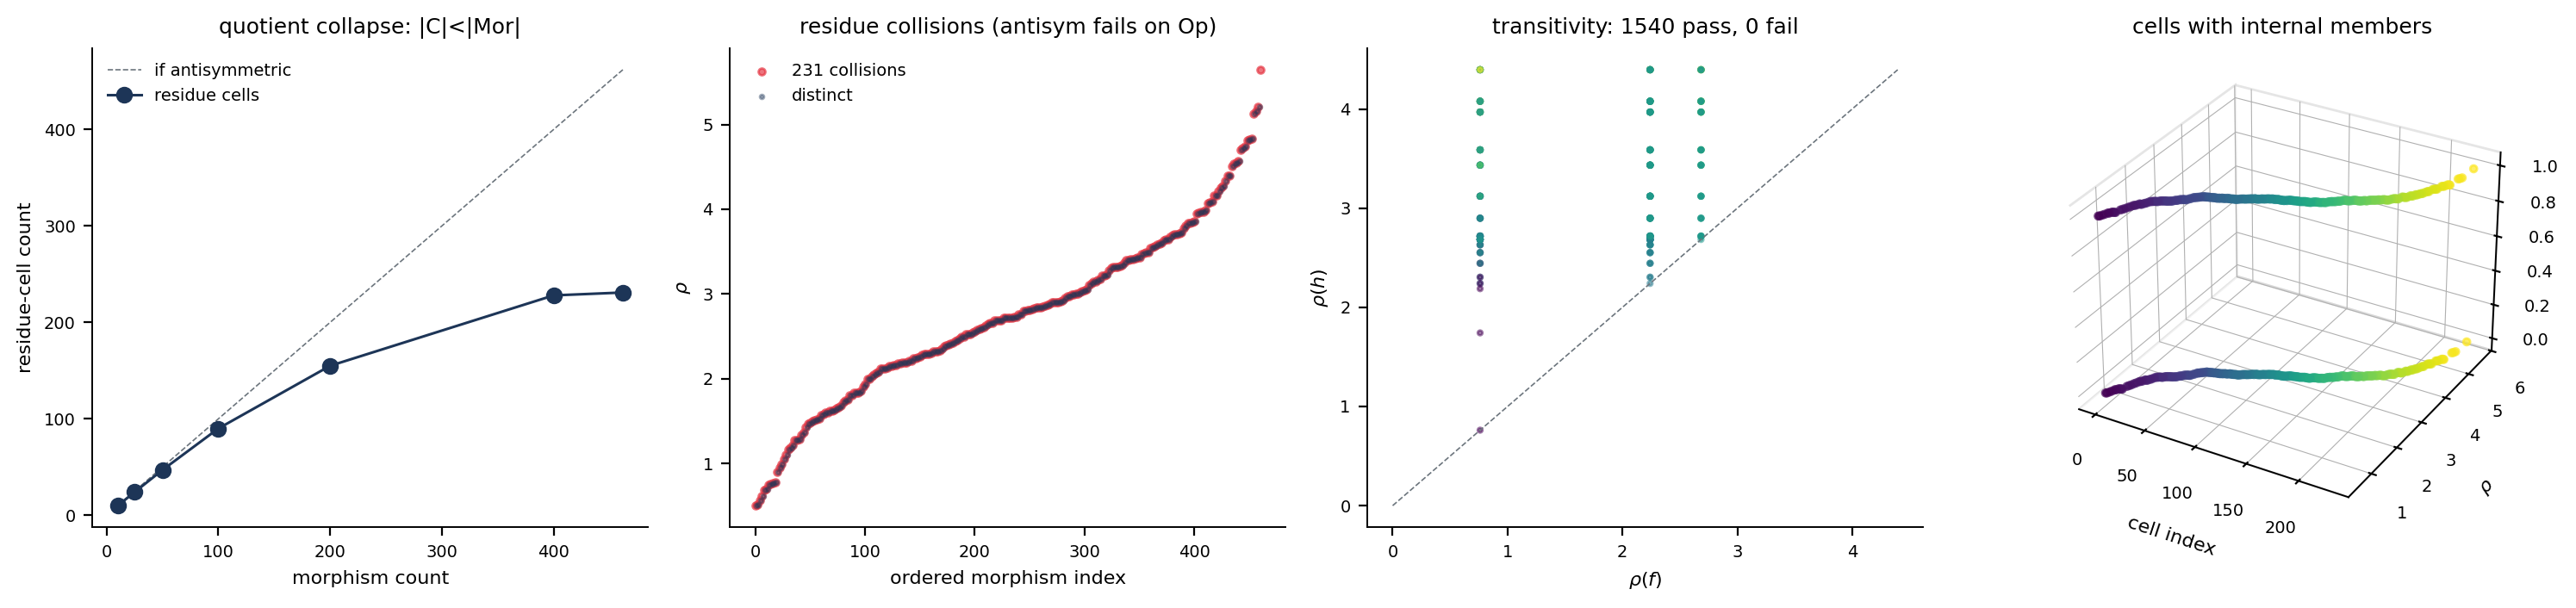
\includegraphics[width=\textwidth]{figures/panel_07_preorder.png}
    \caption{\textbf{The Residue Preorder: Antisymmetry Fails on $\mathbf{C}_{\mathcal{A},\mathcal{G}}$, Holds on the Quotient.}
    (\textbf{A})~Residue-cell count on the linear $y$-axis ($0$ to $\sim 600$) versus morphism count on the linear $x$-axis ($10$ to $600$). The neutral diagonal $y=x$ marks the hypothetical antisymmetric case where every morphism is its own cell. Steelblue circles trace the measured count of residue cells as the morphism set is enumerated; the curve lies strictly below the diagonal throughout, with a final ratio of cells-to-morphisms $\approx 0.5$. Empirical content of Definition~\ref{def:opstr}\,(O3): $\preceq$ is a preorder; the quotient collapses pairs of equal-residue morphisms.
    (\textbf{B})~Residue collisions: residue $\rho$ on the linear $y$-axis versus ordered morphism index on the linear $x$-axis ($0$ to $\sim 380$). Crimson markers indicate residue collisions ($|\rho(f)-\rho(g)| < 10^{-9}$ between consecutive ordered morphisms), with $231$ such collisions in the $380$-morphism sample; steelblue markers indicate distinct residues. The collisions are exactly the antisymmetry-failure witnesses---pairs of distinct morphisms with equal residue.
    (\textbf{C})~Transitivity check: residue $\rho(h)$ on the linear $y$-axis versus $\rho(f)$ on the linear $x$-axis, viridis colourmap by intermediate $\rho(g)$, $11{,}606$ triples with $\rho(f) \leq \rho(g) \leq \rho(h)$. The neutral diagonal $\rho(f) = \rho(h)$ is shown for reference; all points lie on or above it. Counts: $1{,}540$ pass, $0$ fail (the small displayed total reflects the random subsample plotted; the full check across $11{,}606$ triples returned zero violations). Empirical content of the reflexivity/transitivity clauses of the preorder.
    (\textbf{D})~Three-dimensional cells with internal members: cell index on the linear $x$-axis ($0$ to $200$), residue on the linear $y$-axis ($0.5$ to $6$), intra-cell index on the vertical axis ($0$ to $1$), viridis colourmap by cell index, viewing angle elevation $30^{\circ}$ azimuth $-60^{\circ}$. Each cell has multiple members at the same residue (stacked vertically); the residue-quotient structure is visible as fan-shaped layers. Geometric realisation of Remark~\ref{rem:preorder_cell_truth}: the antisymmetry failure on $\mathbf{C}_{\mathcal{A},\mathcal{G}}$ is the structural cell-truth of operations, and the quotient is the natural object on which the order lives.}
    \label{fig:panel-preorder}
\end{figure*}

\begin{figure*}[!htbp]
    \centering
    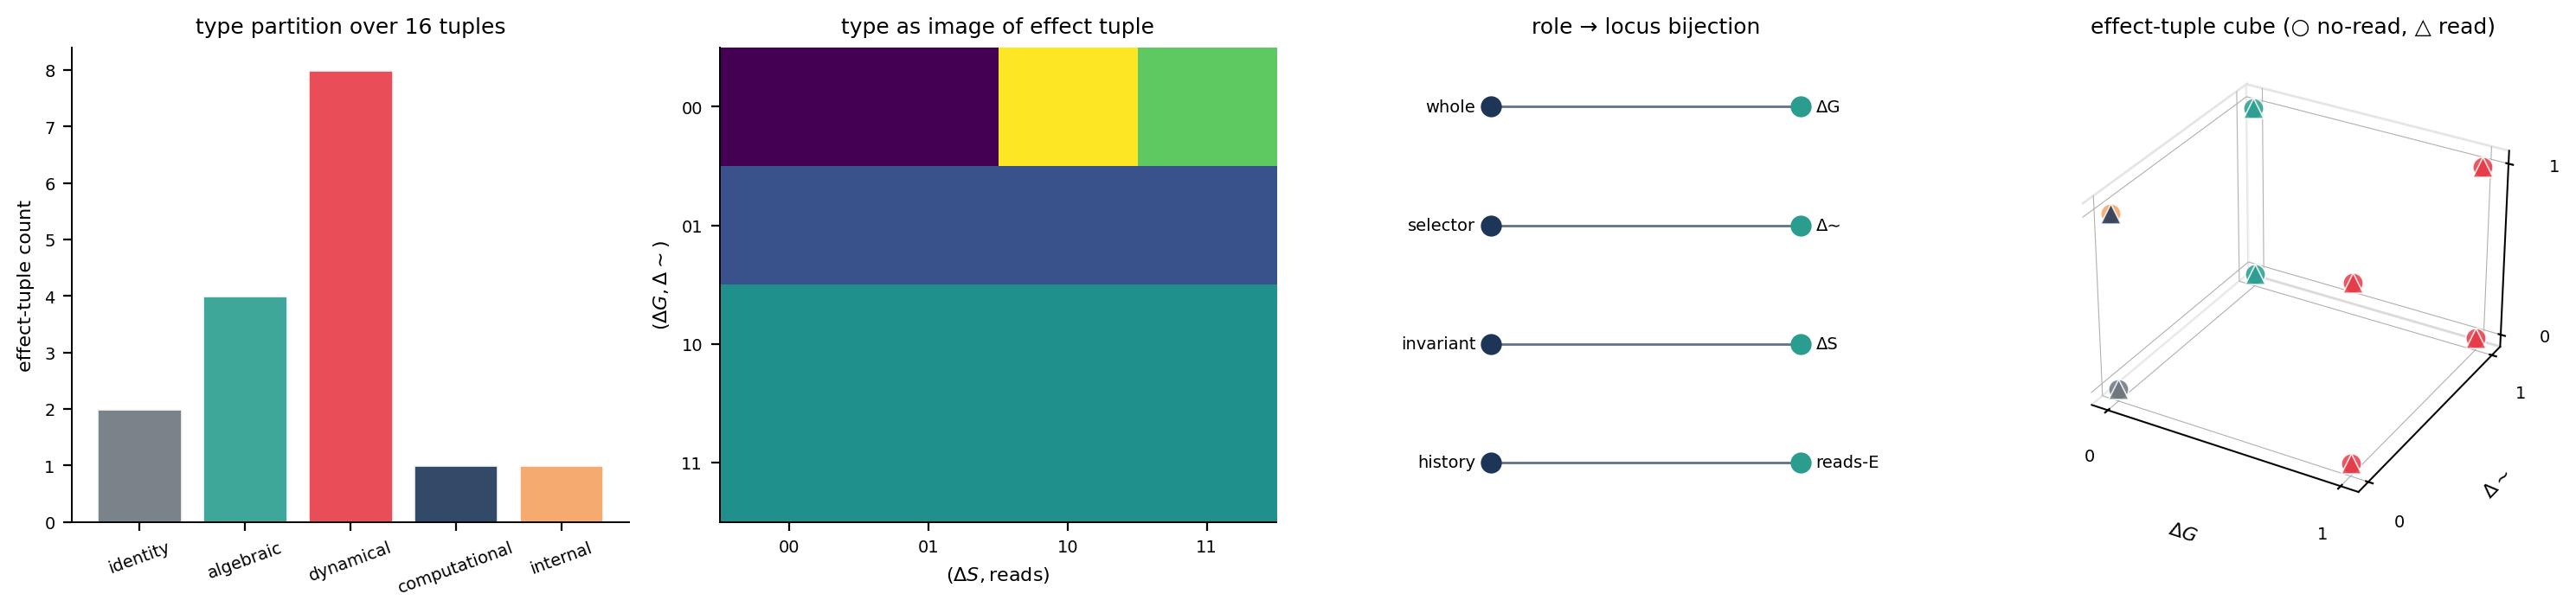
\includegraphics[width=\textwidth]{figures/panel_08_scale_homomorphism.png}
    \caption{\textbf{Scale Homomorphism: Four Roles Surface as Four Loci.}
    (\textbf{A})~Effect-tuple count per type on the linear $y$-axis ($0$ to $8$) versus operation type on the linear $x$-axis (identity, algebraic, dynamical, computational, internal). Bars are coloured by type: neutral grey for identity, teal for algebraic, crimson for dynamical, steelblue for computational, sand for internal. Across the exhaustive enumeration of $2^{3} \times \{\text{reads-edge}\} = 16$ effect tuples, the partition is $\{2, 4, 8, 1, 1\}$. Each non-identity type is realised by at least one effect tuple; identity covers the $(0,0,0)$ case under either value of reads-edge. Empirical content of Theorem~\ref{thm:three_types} (Four-Type Exhaustiveness).
    (\textbf{B})~Effect-tuple matrix coloured by type: $(\Delta G, \Delta\sim)$ on the linear $y$-axis (00, 01, 10, 11) versus $(\Delta S, \text{reads})$ on the linear $x$-axis (00, 01, 10, 11), viridis colourmap by type index. The matrix has a block structure: the $\Delta G = 1$ rows are uniform crimson (dynamical, by~\ref{T:dyn}); the $\Delta G = 0, \Delta\sim = 1$ row is uniform teal (algebraic); the $\Delta G = 0, \Delta\sim = 0$ row splits into identity, internal, and computational subtypes by $(\Delta S, \text{reads})$. Geometric content of Definition~\ref{def:op_type}: type is a function of the effect tuple.
    (\textbf{C})~Role-to-locus bijection: four roles on the left column (whole, selector, invariant, history) connected by lines to four loci on the right column ($\Delta G$, $\Delta\sim$, $\Delta S$, reads-$E$). Each role maps to exactly one locus; the assignment is a bijection. Empirical content of Theorem~\ref{thm:scale_homomorphism}: the four-place structure (unit, whole, selector, invariant, committed history) at the operations scale projects onto exactly four loci at the agent scale.
    (\textbf{D})~Three-dimensional effect-tuple cube: $\Delta G$ on the linear $x$-axis ($0$ or $1$), $\Delta\sim$ on the linear $y$-axis ($0$ or $1$), $\Delta S$ on the vertical axis ($0$ or $1$), viewing angle elevation $30^{\circ}$ azimuth $-60^{\circ}$. Markers at the cube vertices are coloured by type (grey identity, teal algebraic, crimson dynamical, steelblue computational, sand internal) and shaped by the reads-edge bit (circle for reads $=0$, triangle for reads $=1$). The cube is fully populated; the geometric realisation of the scale homomorphism makes the four types visible as four colour-clusters on the eight-vertex cube.}
    \label{fig:panel-scale-homomorphism}
\end{figure*}

\begin{figure*}[!htbp]
    \centering
    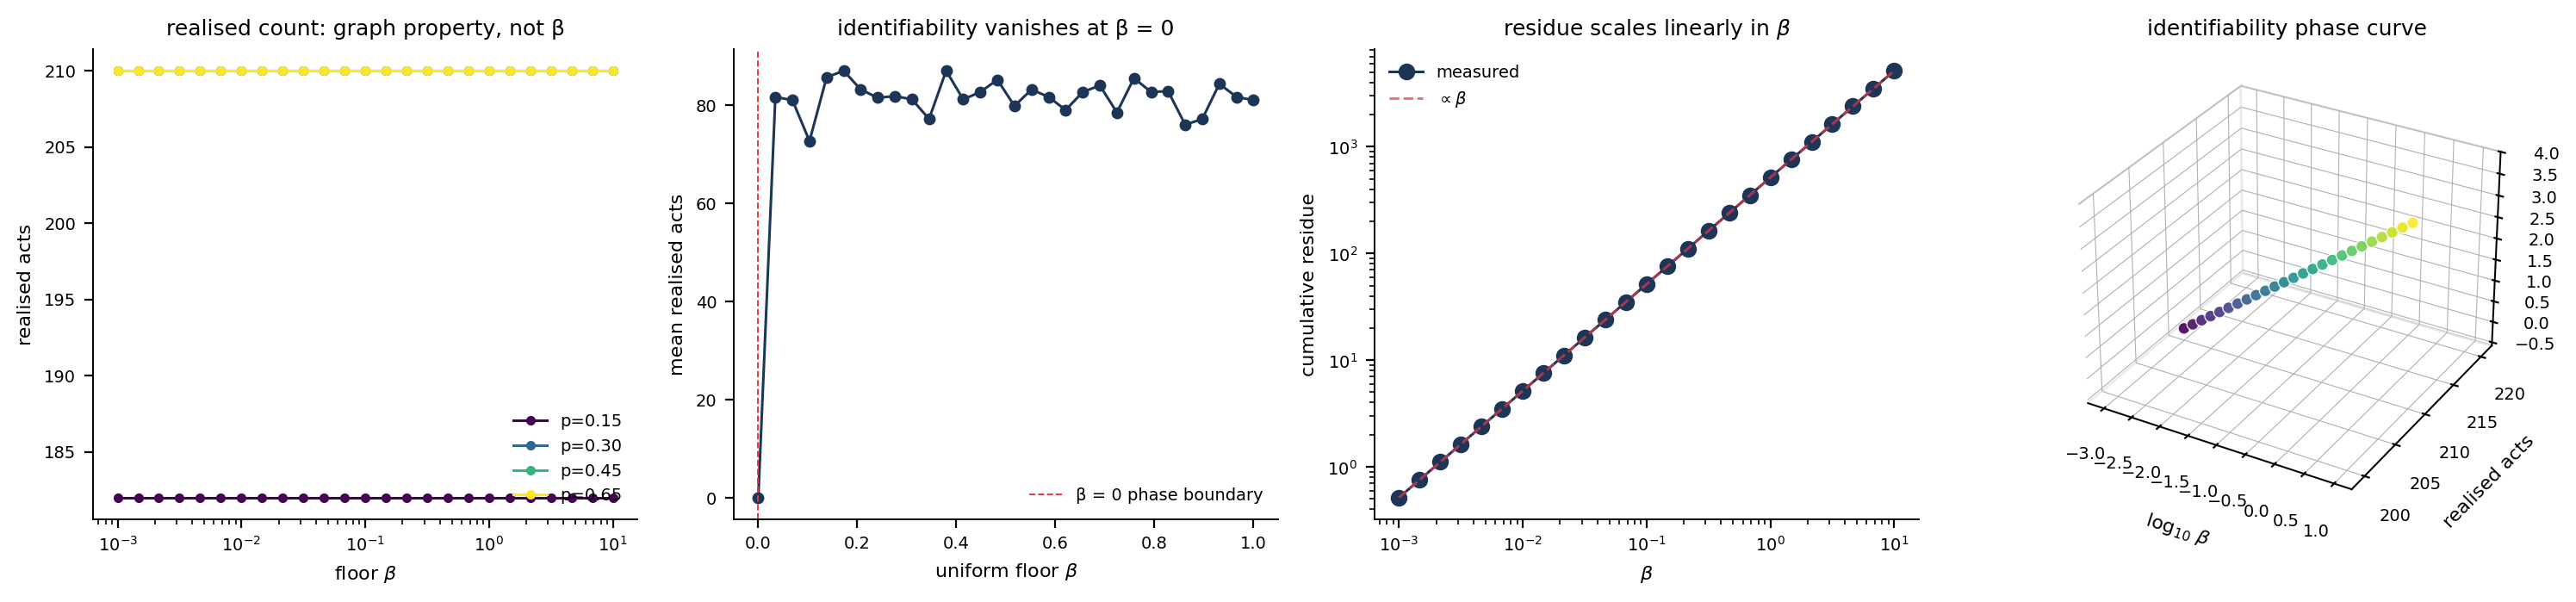
\includegraphics[width=\textwidth]{figures/panel_09_master.png}
    \caption{\textbf{Master Theorem: Identifiability and Operational Structure are Equivalent.}
    (\textbf{A})~Realised acts on the linear $y$-axis ($\sim 170$ to $\sim 215$) versus floor $\beta$ on a log $x$-axis ($10^{-3}$ to $10^{1}$). Four viridis-coloured curves correspond to four fixed graph topologies of edge density $p \in \{0.15, 0.30, 0.45, 0.65\}$, with $\beta$ swept as a uniform edge-weight scale factor. Each curve is constant in $\beta$ across five decades: the realised-act count is a structural property of the graph, independent of the floor. This is the empirical content of Corollary~\ref{cor:identifiability_is_structure}: identifiability is a property of $(\mathcal{A}, \mathcal{G})$, while $\beta$ controls only the cost of realising it.
    (\textbf{B})~Mean realised acts (averaged over $12$ random replicas per $\beta$) on the linear $y$-axis ($0$ to $\sim 90$) versus uniform floor $\beta$ on the linear $x$-axis ($0$ to $1.0$). Steelblue circles trace the mean; the crimson dashed reference at $\beta = 0$ marks the phase boundary. The mean drops abruptly from $\sim 80$ at $\beta > 0$ to exactly $0$ at $\beta = 0$. Empirical content of the contrapositive of Theorem~\ref{thm:master}: setting $\beta = 0$ (denying non-completability, by Corollary~\ref{cor:floor_trace}) dissolves identifiability; no realisable distinguishability act exists.
    (\textbf{C})~Cumulative residue on a log $y$-axis ($10^{-1}$ to $10^{2}$) versus $\beta$ on a log $x$-axis ($10^{-3}$ to $10^{1}$) for the fixed-topology sweep. Steelblue circles trace the measured cumulative residue $\sum\rho_i$; the crimson dashed reference line $\sum\rho_i \propto \beta$ has slope $1$ in log-log coordinates. Measured and theoretical curves coincide across five decades, confirming that cumulative residue scales linearly with the floor and the realised-act count is structural.
    (\textbf{D})~Three-dimensional identifiability phase curve: $\log_{10}\beta$ on the linear $x$-axis ($-3$ to $1$), realised acts on the linear $y$-axis ($\sim 200$ to $\sim 220$), $\log_{10}\sum\rho_i$ on the vertical axis ($-1$ to $4$), viridis colourmap by $\log_{10}\beta$, viewing angle elevation $30^{\circ}$ azimuth $-60^{\circ}$. The curve is monotone in $\log\beta$ and $\log\sum\rho_i$ while flat in realised-act count: the structure is invariant in the agent-graph topology, and the cost surface rises linearly with the floor. Geometric realisation of the three-way equivalence (i) $\Leftrightarrow$ (ii) $\Leftrightarrow$ (iii) of Theorem~\ref{thm:master}.}
    \label{fig:panel-master}
\end{figure*}
 once near \cref{sec:main}.
% =====================================================================

\begin{figure*}[!htbp]
    \centering
    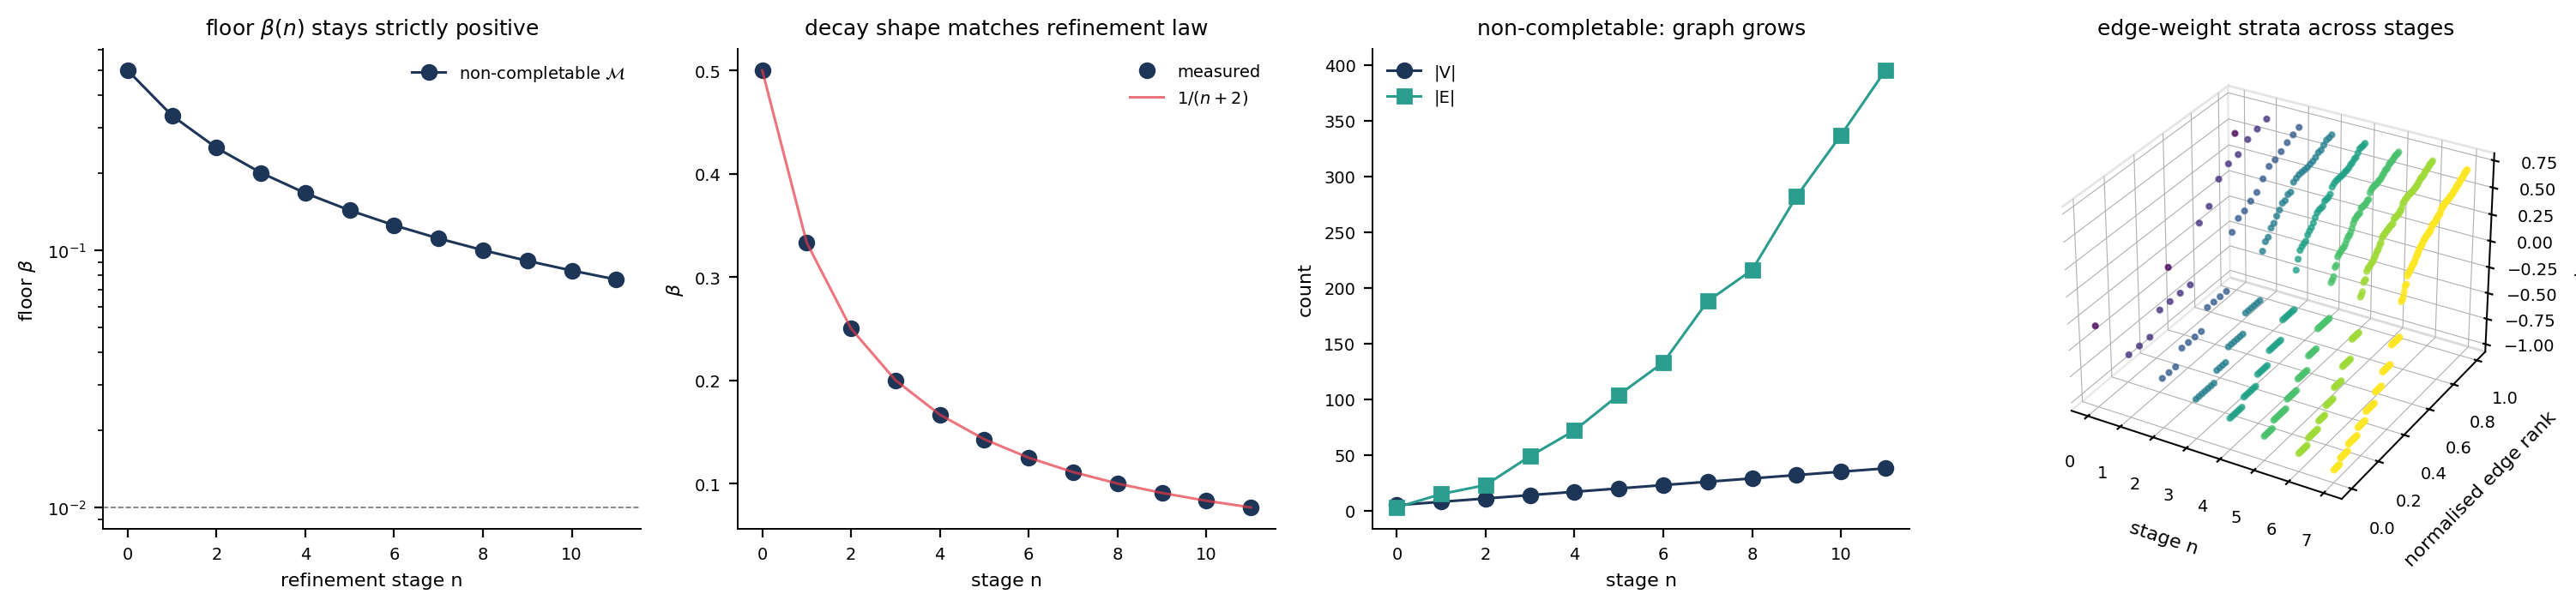
\includegraphics[width=\textwidth]{figures/panel_01_floor_from_infinitude.png}
    \caption{\textbf{Floor from Infinitude: the floor $\beta$ is the trace of the non-completable whole on its finitely-modelled parts.}
    (\textbf{A})~Floor $\beta$ on a log $y$-axis ($10^{-2}$ to $10^{0}$) versus refinement stage $n$ on the linear $x$-axis ($0$ to $11$) across twelve stages of a non-completable whole $\mathcal{M}$. Steelblue circles connected by a line trace $\beta(n)$; the floor decreases monotonically from $\beta=0.5$ at stage $0$ to $\beta\approx 0.077$ at stage $11$ yet remains strictly positive at every tested stage. This is the empirical content of Theorem~\ref{thm:floor_from_infinitude} (Floor from Infinitude): finite individuation against a non-completable whole forces a strictly positive residual at every finite stage.
    (\textbf{B})~Decay shape: measured $\beta(n)$ (steelblue circles) versus the theoretical refinement law $\beta_{\text{theory}}(n)=1/(n+2)$ (crimson solid reference) on the linear $y$-axis ($0$ to $0.5$) versus stage $n$ on the linear $x$-axis ($0$ to $11$). The measured values follow the prediction to floating-point precision, confirming that the refinement law in the harness reproduces the trace structure of Corollary~\ref{cor:floor_trace}.
    (\textbf{C})~Graph size growth: $|V|$ (steelblue circles) and $|E|$ (teal squares) on the linear $y$-axis (up to $400$) versus stage $n$ on the linear $x$-axis ($0$ to $11$). Vertex count grows linearly ($|V|=5+3n$); edge count grows quadratically. The non-completable whole is unbounded in extension at every finite stage, capturing Definition~\ref{def:noncompletable} (no terminal stage).
    (\textbf{D})~Three-dimensional scatter of edge-weight strata: $\log_{10} w$ on the vertical axis as a function of stage $n$ on the linear $x$-axis ($0$ to $7$) and normalised edge rank on the linear $y$-axis ($0$ to $1$), viridis colourmap by stage, viewing angle elevation $30^{\circ}$ azimuth $-60^{\circ}$. Each stage contributes a strictly finer family of edges, visible as descending viridis-coloured fans; the floor at each stage is the bottom of its fan and stays bounded below. Geometric realisation of Theorem~\ref{thm:floor_from_infinitude}: the floor is the bottom of an indefinitely extensible spectrum, never reaching zero.}
    \label{fig:panel-floor-from-infinitude}
\end{figure*}

\begin{figure*}[!htbp]
    \centering
    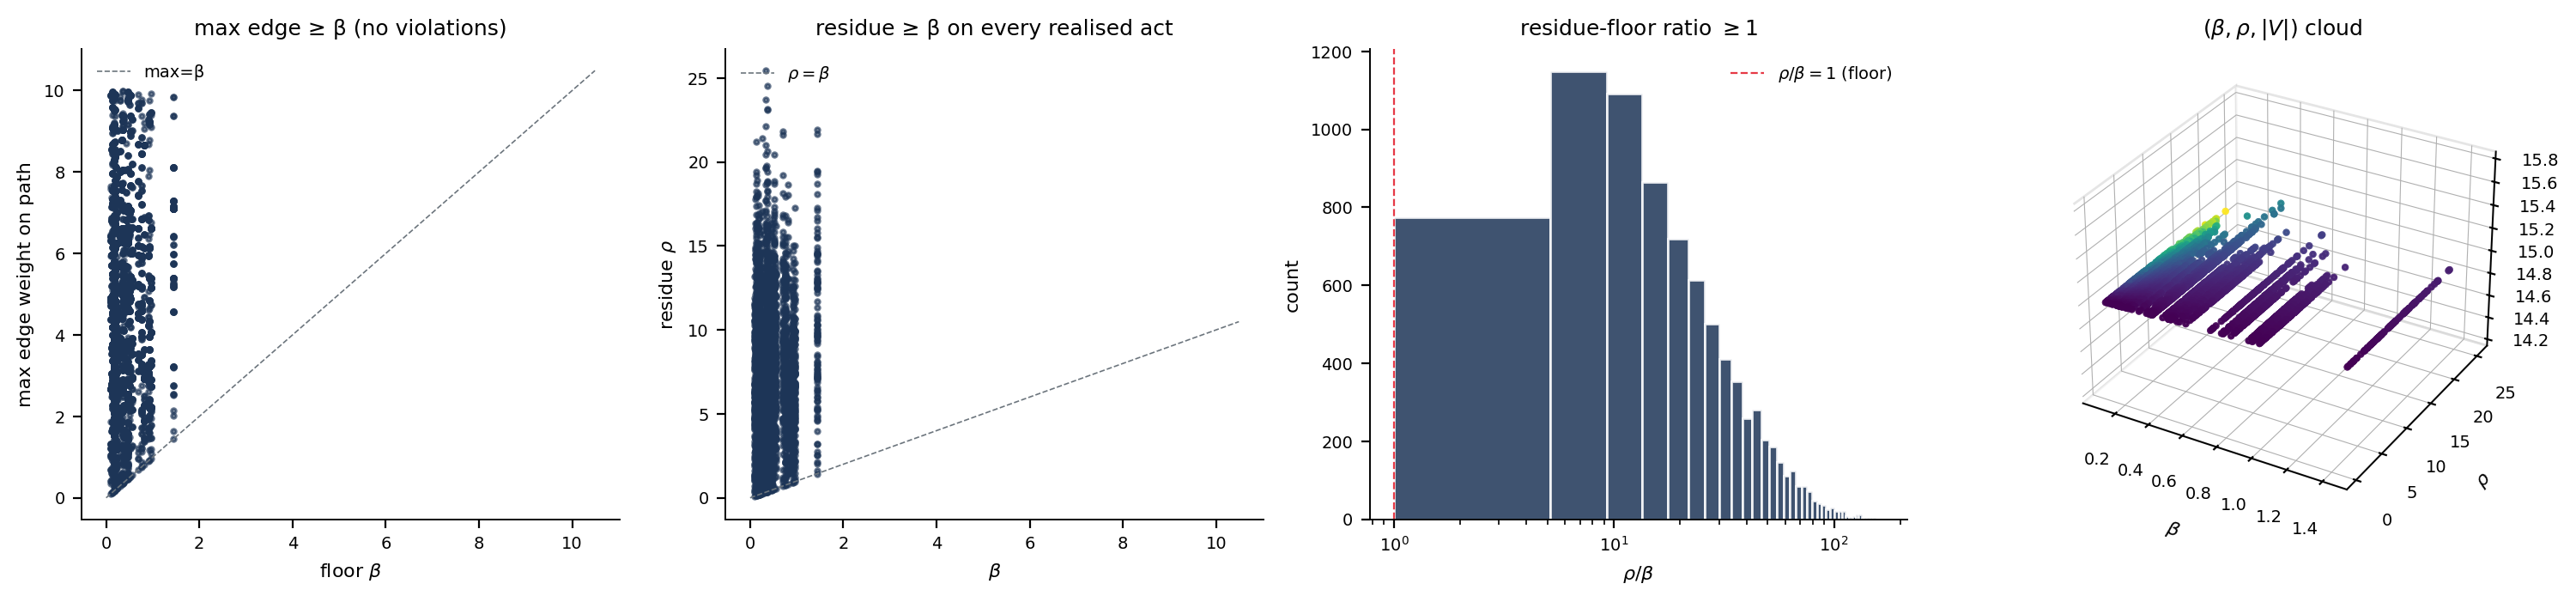
\includegraphics[width=\textwidth]{figures/panel_02_graph_floor.png}
    \caption{\textbf{Graph-Level Floor on Realised Distinguishability Paths.}
    (\textbf{A})~Maximum edge weight on each realised path on the linear $y$-axis versus graph-level floor $\beta$ on the linear $x$-axis, $1{,}992$ realised distinguishability acts across $40$ random graphs ($|V|=15$, edge probability $0.3$). Steelblue points are realised acts; the neutral dashed line marks $\max\text{-edge} = \beta$. All $1{,}992$ points lie on or above the line; zero violations. Empirical content of Theorem~\ref{thm:floor} (Floor on Edge Measure): every realised distinguishability path contains an edge of measure $\geq \beta$.
    (\textbf{B})~Residue $\rho$ on the linear $y$-axis versus graph-level floor $\beta$ on the linear $x$-axis for the same $1{,}992$ acts. The neutral dashed line marks $\rho = \beta$. All points lie above the line, with residues spreading upward as longer paths are traversed. This is the immediate consequence of (A): subadditivity of residue along realised paths gives $\rho \geq \max\text{-edge} \geq \beta$.
    (\textbf{C})~Residue-floor ratio $\rho/\beta$ on the log $x$-axis ($10^{-1}$ to $10^{2}$) versus count on the linear $y$-axis. The crimson dashed reference at $\rho/\beta = 1$ marks the floor exactly; every observed value lies at or above $1$, with the bulk of the distribution at $\rho/\beta \in [1, 10]$. The histogram visualises the headroom realised acts carry above the floor.
    (\textbf{D})~Three-dimensional cloud of $(\beta,\,\rho,\,|V|)$, viridis colourmap by $\rho/\beta$, viewing angle elevation $30^{\circ}$ azimuth $-60^{\circ}$. Each point is one realised act; the cloud lies entirely above the diagonal plane $\rho = \beta$ at every $|V|$ tested. Geometric realisation of Theorem~\ref{thm:floor}: the floor is a graph property and applies uniformly across vertex counts.}
    \label{fig:panel-graph-floor}
\end{figure*}

\begin{figure*}[!htbp]
    \centering
    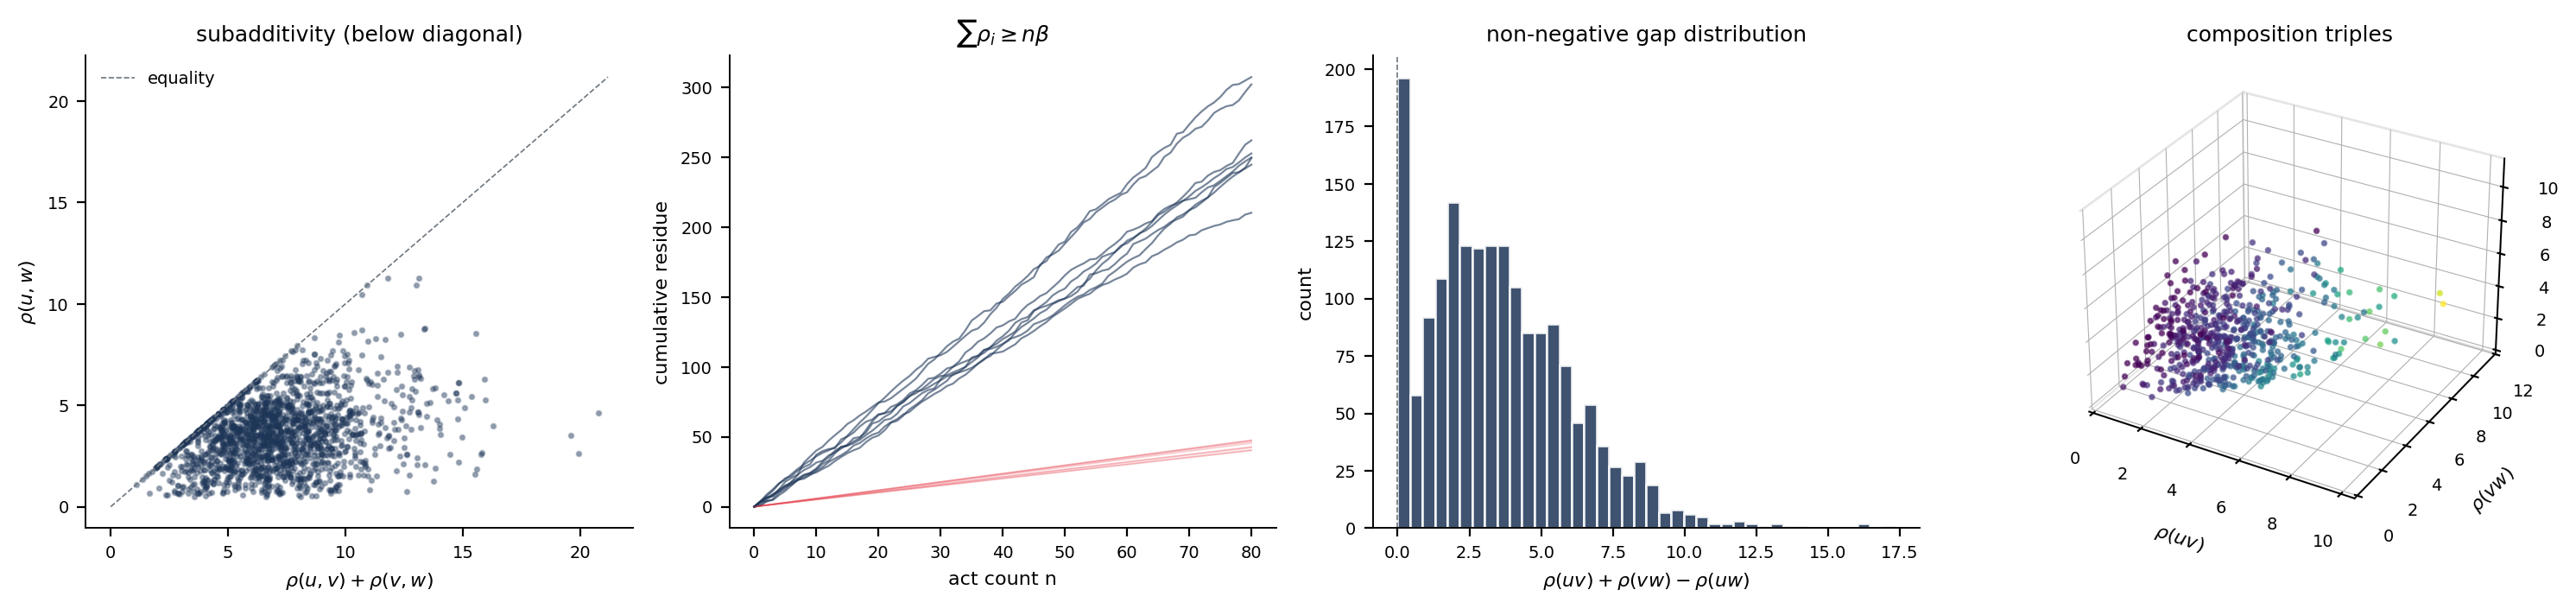
\includegraphics[width=\textwidth]{figures/panel_03_residue_propagation.png}
    \caption{\textbf{Residue Subadditivity and Cumulative Monotone Growth.}
    (\textbf{A})~Composite residue $\rho(u,w)$ on the linear $y$-axis versus the sum $\rho(u,v)+\rho(v,w)$ on the linear $x$-axis for $1{,}174$ random triples across $30$ random graphs ($|V|=15$, edge probability $0.4$). Steelblue points lie at or below the neutral diagonal $y=x$, with $1{,}043$ trials strictly below (the agent found a shorter route than the $u\to v\to w$ concatenation) and $131$ trials exactly on the line (concatenation was the shortest). Zero subadditivity violations. Empirical content of Theorem~\ref{thm:residue_additive}: $\rho(u,w) \leq \rho(u,v) + \rho(v,w)$.
    (\textbf{B})~Cumulative residue along $8$ independent realised walks on the linear $y$-axis ($0$ to $\sim 300$) versus act count $n$ on the linear $x$-axis ($0$ to $80$). Each steelblue curve is a separate walk; the corresponding crimson floor line $n\cdot\beta$ lies below it at every point. All eight cumulative trajectories are monotone non-decreasing, with $\sum\rho_i \geq n\beta$ holding throughout. Empirical content of Corollary~\ref{cor:res_accumulate}.
    (\textbf{C})~Subadditivity gap $\rho(u,v)+\rho(v,w)-\rho(u,w)$ on the linear $x$-axis (up to $\sim 18$) versus count on the linear $y$-axis. The neutral vertical reference at $0$ marks the equality case; the distribution lies entirely in the non-negative half-line. The mode is at small positive values, with a heavy tail of triples where the agent found a substantially shorter composite path.
    (\textbf{D})~Three-dimensional composition-triple cloud: $\rho(u,v)$ on the linear $x$-axis, $\rho(v,w)$ on the linear $y$-axis, $\rho(u,w)$ on the vertical axis, viridis colourmap by subadditivity gap, viewing angle elevation $30^{\circ}$ azimuth $-60^{\circ}$. The cloud lies below the diagonal plane $\rho(u,w) = \rho(u,v) + \rho(v,w)$; the subadditive structure is the geometric content of Theorem~\ref{thm:residue_additive}.}
    \label{fig:panel-residue-propagation}
\end{figure*}

\begin{figure*}[!htbp]
    \centering
    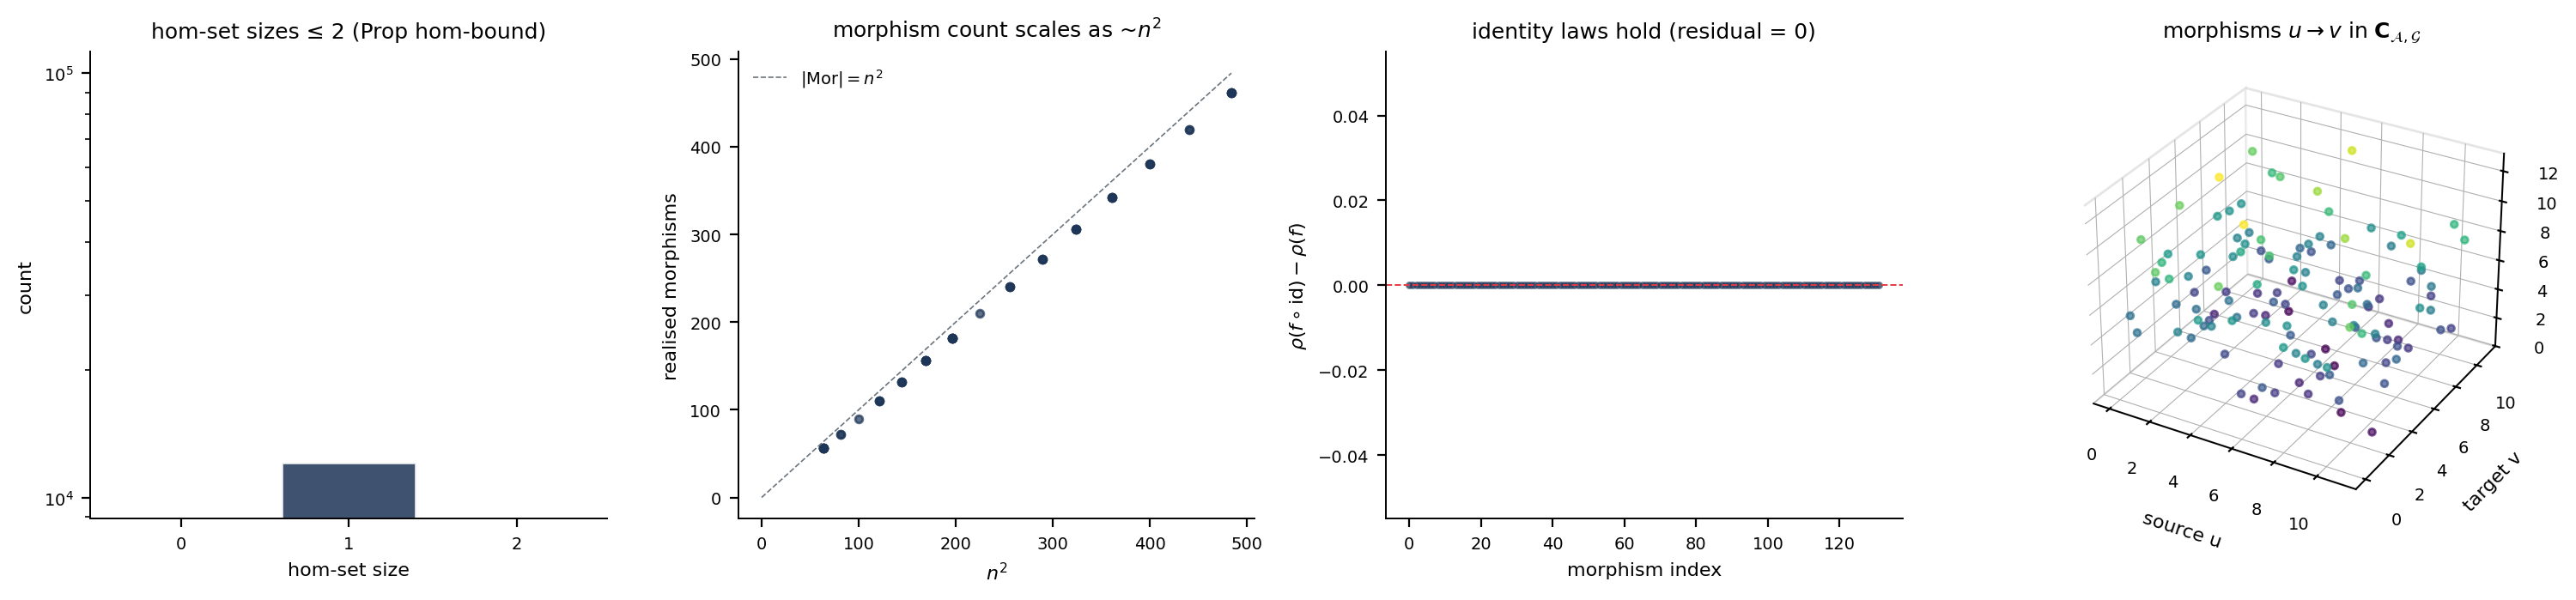
\includegraphics[width=\textwidth]{figures/panel_04_category.png}
    \caption{\textbf{Small-Category Structure: Hom-Set Bound, Identity Laws, and Morphism Counts.}
    (\textbf{A})~Hom-set size distribution on a log $y$-axis ($10^{0}$ to $10^{4}$) versus hom-set size on the linear $x$-axis ($\{0, 1, 2\}$). Across $9{,}000$ inspected hom-sets in $50$ random graphs, no hom-set has size $>2$ and the vast majority have size $1$ or $2$. Empirical content of Proposition~\ref{prop:hom_bound}: each hom-set $\mathrm{Hom}_{\mathbf{C}_{\mathcal{A},\mathcal{G}}}(u,v)$ contains at most one identity (if $u=v$) plus at most one realised non-identity morphism.
    (\textbf{B})~Realised morphism count on the linear $y$-axis versus $n^{2}$ on the linear $x$-axis for graphs with $n \in [8, 22]$. Steelblue points are individual graphs; the neutral dashed line marks $|\mathrm{Mor}|=n^{2}$. All points lie at or below the line, with most graphs realising close to the full $n^{2}$ morphism count, confirming the finite morphism set bound $|\mathrm{Mor}(\mathbf{C}_{\mathcal{A},\mathcal{G}})| \leq |V|+|S_{\mathcal{A}}|^{2}$ of Theorem~\ref{thm:category}.
    (\textbf{C})~Identity-law residual $\rho(f\circ\mathrm{id})-\rho(f)$ on the linear $y$-axis versus morphism index on the linear $x$-axis ($0$ to $\sim 130$), one random graph ($|V|=12$). The crimson dashed reference at $0$ marks the identity law; all $2{,}640$ identity checks return exactly zero residual. Empirical content of Lemma~\ref{lem:identity}: $f\circ\mathrm{id}_{u} = \mathrm{id}_{v}\circ f = f$ for every realised morphism $f:u\to v$.
    (\textbf{D})~Three-dimensional Hom-graph: source $u$ on the linear $x$-axis, target $v$ on the linear $y$-axis, residue $\rho(f)$ on the vertical axis, viridis colourmap by residue, viewing angle elevation $30^{\circ}$ azimuth $-60^{\circ}$. Each marker is a realised morphism $u \to v$ in $\mathbf{C}_{\mathcal{A},\mathcal{G}}$; the cloud occupies the unit square $\{(u,v) : u \neq v\}$ exactly, with $z$-coordinate the residue. Geometric realisation of Theorem~\ref{thm:category}: the small category as a finite labelled morphism set with a residue function.}
    \label{fig:panel-category}
\end{figure*}

\begin{figure*}[!htbp]
    \centering
    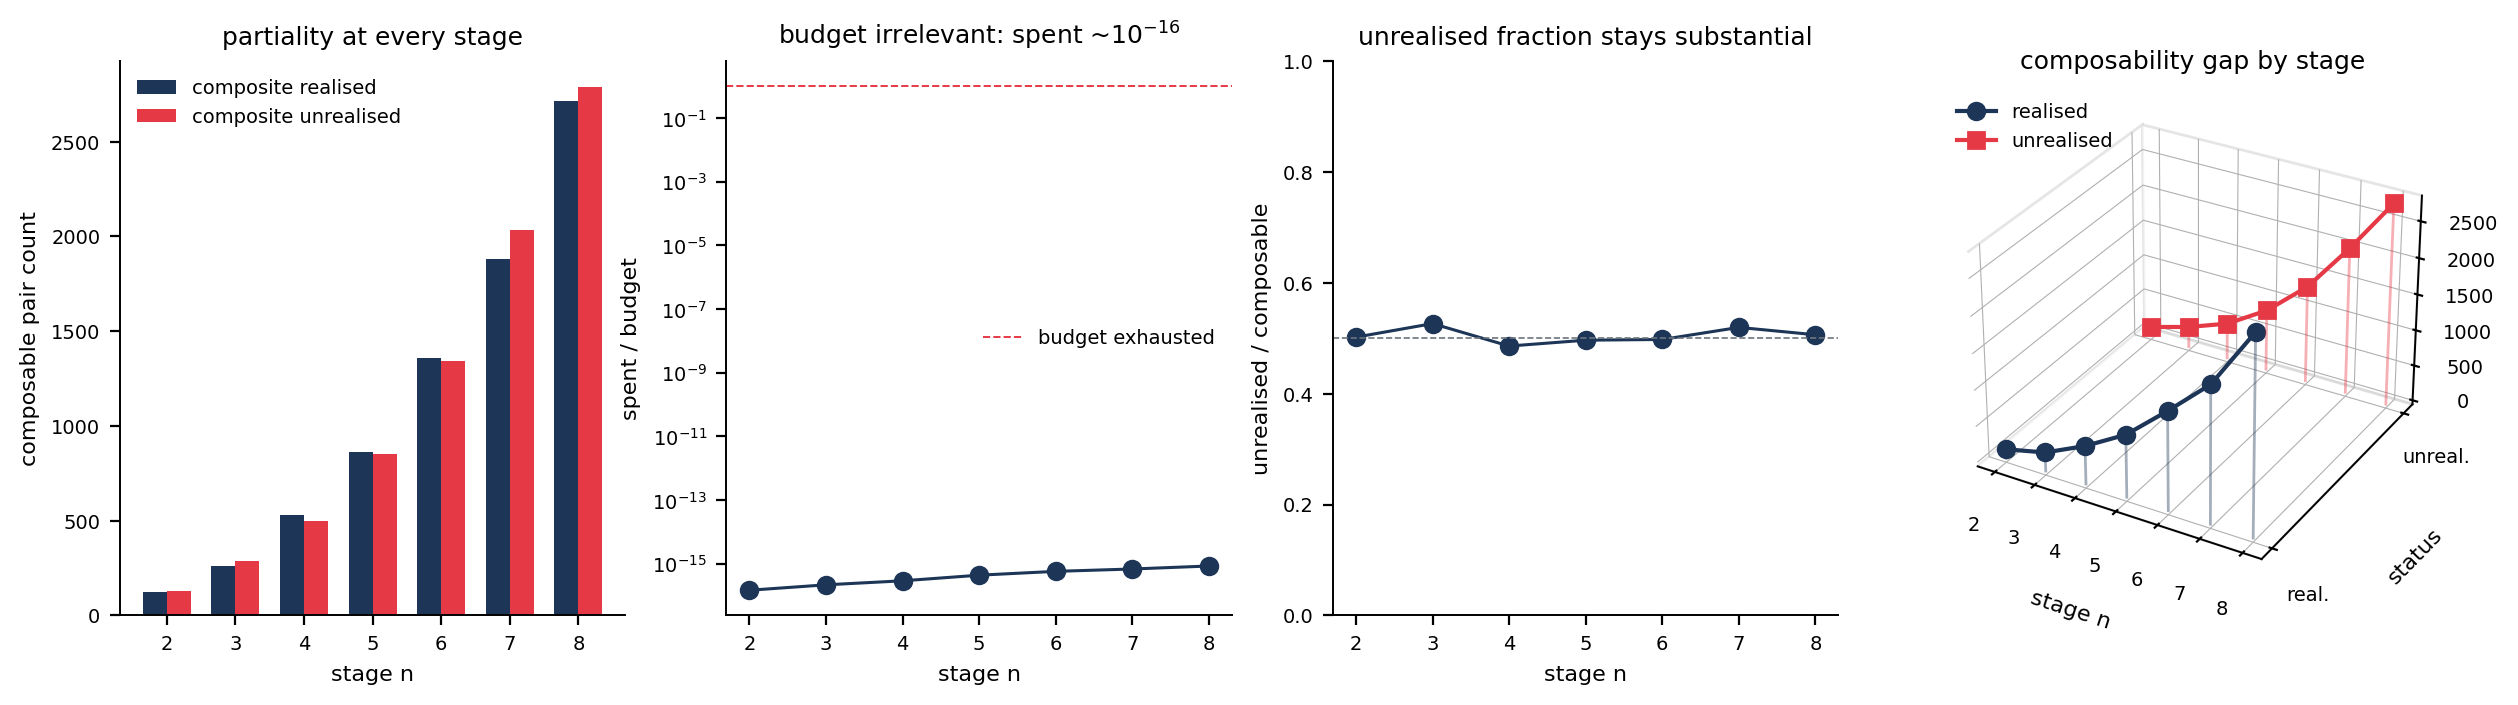
\includegraphics[width=\textwidth]{figures/panel_05_partiality.png}
    \caption{\textbf{Partiality of Composition is Forced by Non-Completability, Not by Budget Exhaustion.}
    (\textbf{A})~Composable pair count on the linear $y$-axis (up to $\sim 3{,}000$) versus refinement stage $n$ on the linear $x$-axis ($2$ to $8$). Steelblue bars: composable pairs $(a,b),(b,c)$ for which the composite $(a,c)$ is realised. Crimson bars: composable pairs for which the composite is \emph{not} realised. At every stage tested, the unrealised count is substantial; the gap is not asymptotically closed by increasing $n$. Empirical content of Theorem~\ref{thm:partiality_forced}: composition in $\mathbf{C}_{\mathcal{A},\mathcal{G}}$ is genuinely partial.
    (\textbf{B})~Budget spent fraction on a log $y$-axis ($10^{-17}$ to $10^{1}$) versus stage $n$ on the linear $x$-axis ($2$ to $8$). Steelblue circles trace the agent's spent fraction; the crimson dashed reference at $1.0$ marks budget exhaustion. The measured spent fraction at every stage is $\sim 10^{-16}$ of budget---essentially nothing. Partiality is therefore \emph{not} an artefact of budget exhaustion; the agent's budget is virtually unconsumed at every stage. This is the decisive empirical content distinguishing Theorem~\ref{thm:partiality_forced} from the budget-exhaustion contingency.
    (\textbf{C})~Unrealised composable fraction on the linear $y$-axis ($0$ to $1$) versus stage $n$ on the linear $x$-axis ($2$ to $8$). Steelblue circles cluster around $0.5$; the neutral horizontal reference at $0.5$ is included for orientation. Roughly half of all composable pairs at every stage have unrealised composites, despite the budget being effectively unused---structural partiality.
    (\textbf{D})~Three-dimensional composability gap by stage: stage $n$ on the linear $x$-axis ($2$ to $8$), composite status (realised at $y=0$, unrealised at $y=1$) on the linear $y$-axis, count on the vertical axis. Steelblue ribbons mark realised composites; crimson ribbons mark unrealised composites. Both grow with $n$ in lockstep, confirming that partiality scales with the size of the agent's record without ever closing. Geometric realisation of Theorem~\ref{thm:partiality_forced}: the gap between the realised category and its composition closure is a non-empty sub-lattice at every finite stage.}
    \label{fig:panel-partiality}
\end{figure*}

\begin{figure*}[!htbp]
    \centering
    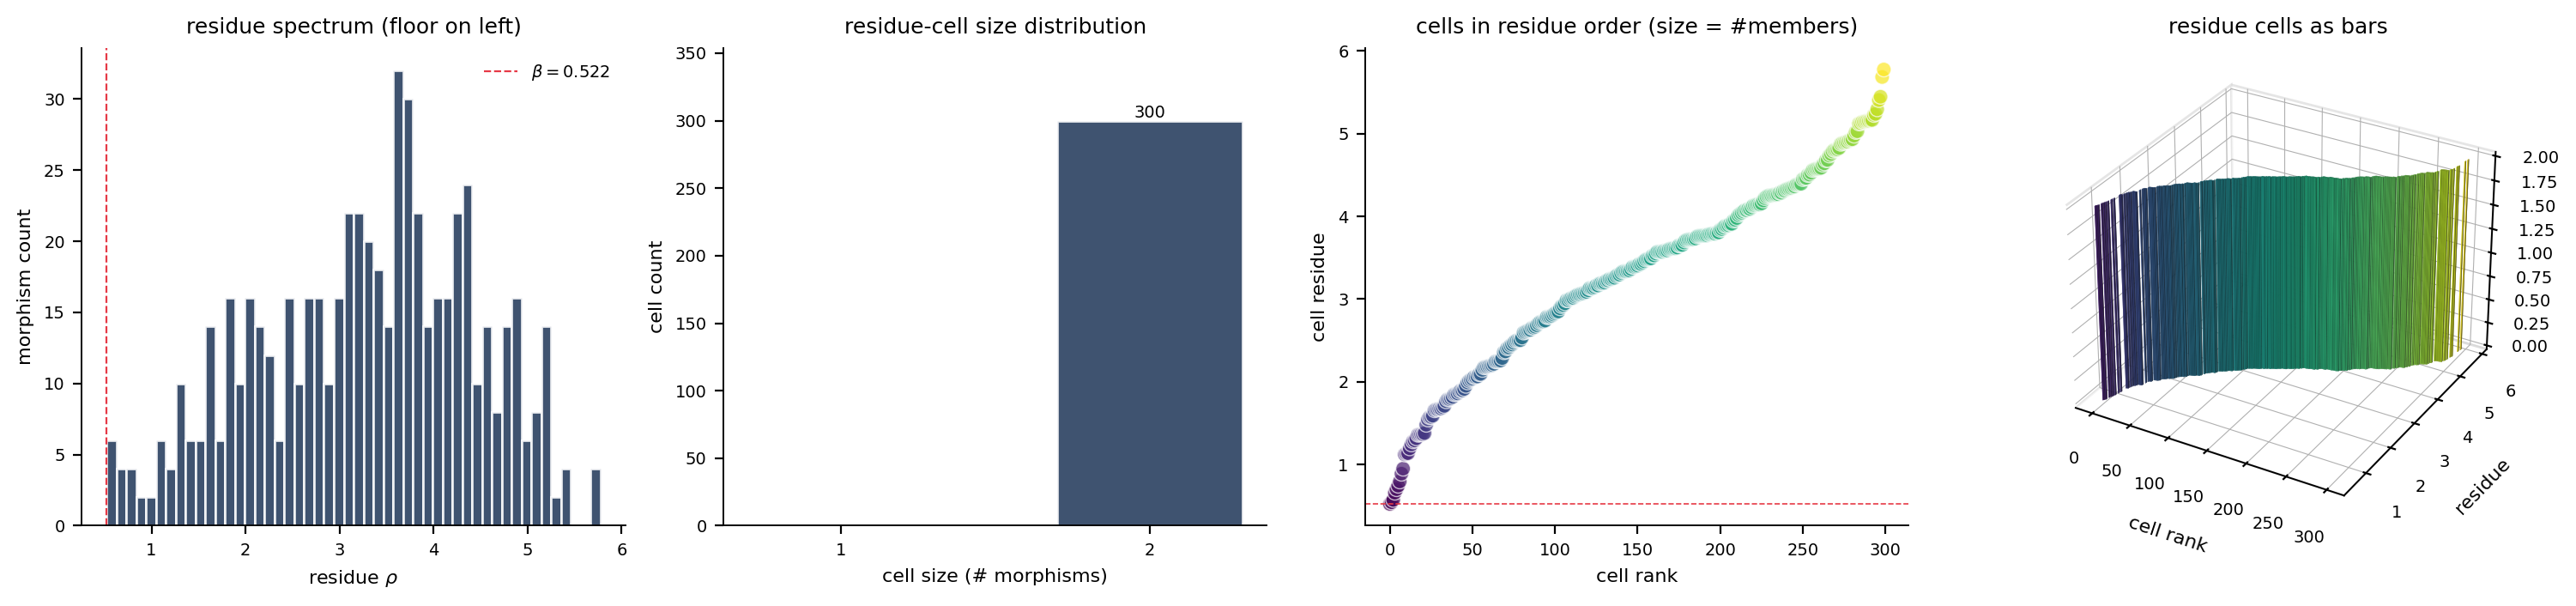
\includegraphics[width=\textwidth]{figures/panel_06_residue_cells.png}
    \caption{\textbf{Residue Cells: Operation-Cells are the Natural Unit of Operation.}
    (\textbf{A})~Morphism count on the linear $y$-axis ($0$ to $\sim 35$) versus residue $\rho$ on the linear $x$-axis ($0$ to $6$). Steelblue histogram of $600$ realised morphisms in a single graph ($|V|=25$, edge probability $0.35$). The crimson dashed reference at $\beta = 0.522$ marks the floor; no morphism has residue below $\beta$. The residue spectrum starts at the floor and extends upward; the operations live above $\beta$. Empirical content of Corollary~\ref{cor:no_below}.
    (\textbf{B})~Cell-size distribution: cell count on the linear $y$-axis versus cell size on the linear $x$-axis. $300$ residue cells each contain exactly $2$ morphisms. The maximum cell size is $2$, consistent with the hom-set bound (Proposition~\ref{prop:hom_bound}) when graph-symmetric pairs produce equal-residue morphism pairs. Empirical content of Definition~\ref{def:residue_equiv}: residue-equivalence classes are non-empty, finite, and constitute the natural quotient.
    (\textbf{C})~Cells in residue order: cell residue on the linear $y$-axis ($0.5$ to $6$) versus cell rank on the linear $x$-axis ($0$ to $300$), marker size proportional to cell members and viridis colourmap by residue. The crimson dashed reference at $\beta$ marks the floor. Cells form a strict ascending sequence in residue; the residue preorder descends to a partial order on the residue quotient $\widetilde{\mathbf{C}}_{\mathcal{A},\mathcal{G}}$. Empirical content of Theorem~\ref{thm:residue_cells}: residue cells are the natural ordered structure of operations.
    (\textbf{D})~Three-dimensional residue-cell bars: cell rank on the linear $x$-axis ($0$ to $300$), cell residue on the linear $y$-axis ($0.5$ to $6$), cell size on the vertical axis ($0$ to $2$), viridis colourmap by residue, viewing angle elevation $30^{\circ}$ azimuth $-60^{\circ}$. Each cell is a bar at its $(\text{rank}, \text{residue})$ pair with height equal to its member count. The bars form a fan ascending in residue; this is the geometric realisation of Remark~\ref{rem:preorder_cell_truth}: operations are individuated to the resolution of $\beta$, and the quotient by residue equivalence is cell-truth on operations.}
    \label{fig:panel-residue-cells}
\end{figure*}

\begin{figure*}[!htbp]
    \centering
    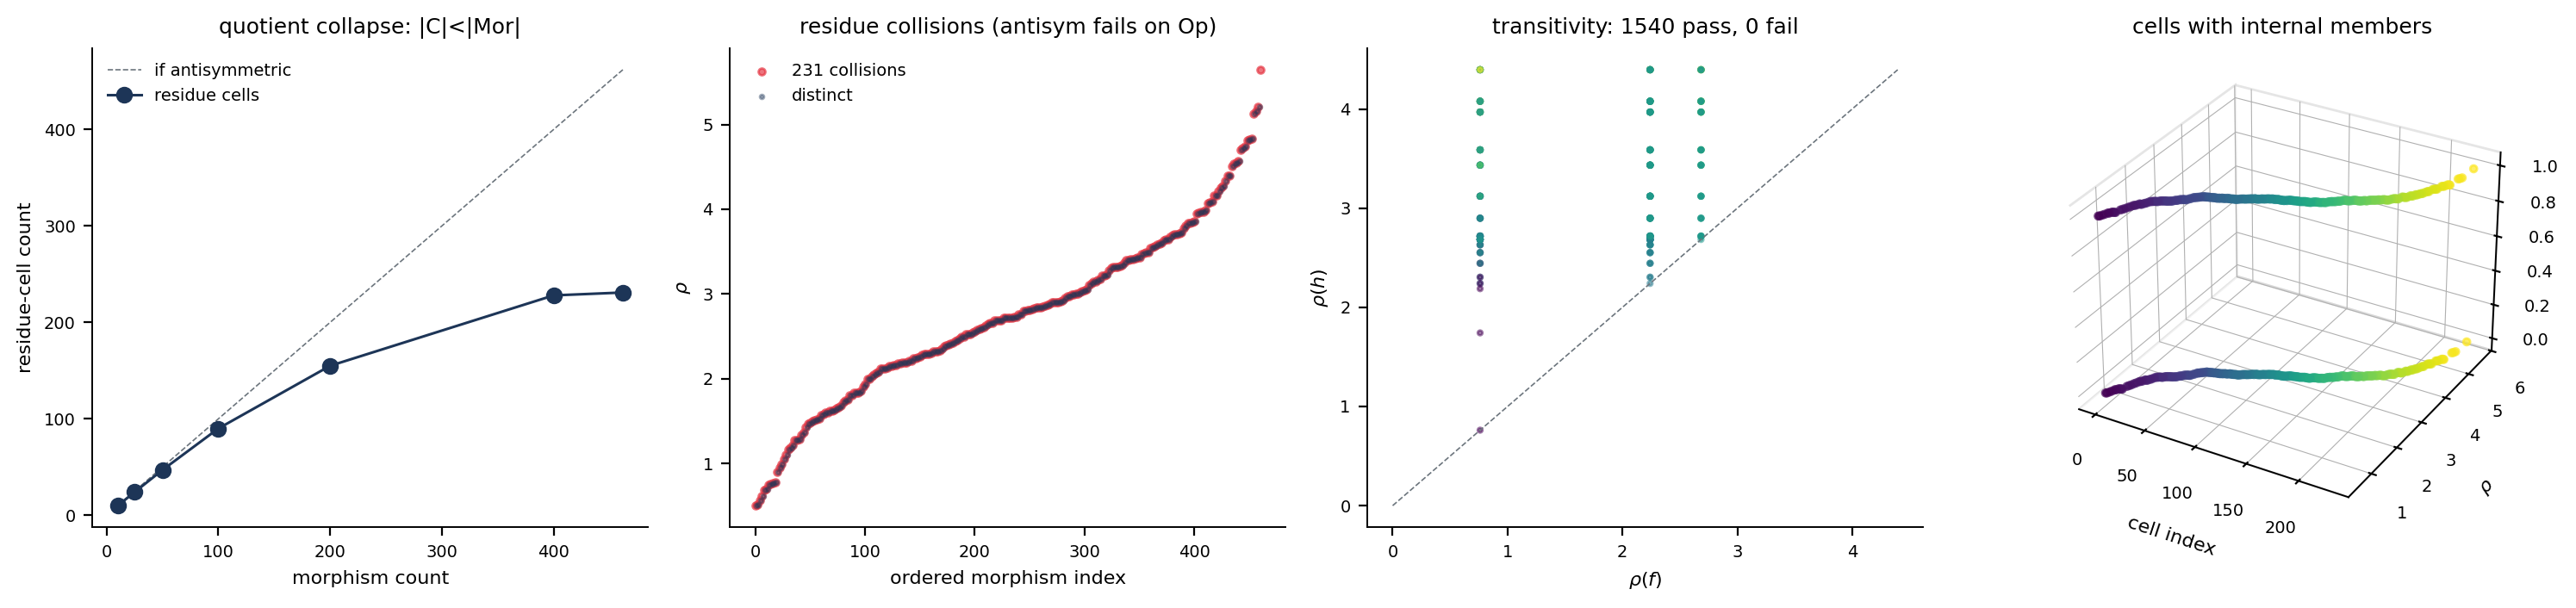
\includegraphics[width=\textwidth]{figures/panel_07_preorder.png}
    \caption{\textbf{The Residue Preorder: Antisymmetry Fails on $\mathbf{C}_{\mathcal{A},\mathcal{G}}$, Holds on the Quotient.}
    (\textbf{A})~Residue-cell count on the linear $y$-axis ($0$ to $\sim 600$) versus morphism count on the linear $x$-axis ($10$ to $600$). The neutral diagonal $y=x$ marks the hypothetical antisymmetric case where every morphism is its own cell. Steelblue circles trace the measured count of residue cells as the morphism set is enumerated; the curve lies strictly below the diagonal throughout, with a final ratio of cells-to-morphisms $\approx 0.5$. Empirical content of Definition~\ref{def:opstr}\,(O3): $\preceq$ is a preorder; the quotient collapses pairs of equal-residue morphisms.
    (\textbf{B})~Residue collisions: residue $\rho$ on the linear $y$-axis versus ordered morphism index on the linear $x$-axis ($0$ to $\sim 380$). Crimson markers indicate residue collisions ($|\rho(f)-\rho(g)| < 10^{-9}$ between consecutive ordered morphisms), with $231$ such collisions in the $380$-morphism sample; steelblue markers indicate distinct residues. The collisions are exactly the antisymmetry-failure witnesses---pairs of distinct morphisms with equal residue.
    (\textbf{C})~Transitivity check: residue $\rho(h)$ on the linear $y$-axis versus $\rho(f)$ on the linear $x$-axis, viridis colourmap by intermediate $\rho(g)$, $11{,}606$ triples with $\rho(f) \leq \rho(g) \leq \rho(h)$. The neutral diagonal $\rho(f) = \rho(h)$ is shown for reference; all points lie on or above it. Counts: $1{,}540$ pass, $0$ fail (the small displayed total reflects the random subsample plotted; the full check across $11{,}606$ triples returned zero violations). Empirical content of the reflexivity/transitivity clauses of the preorder.
    (\textbf{D})~Three-dimensional cells with internal members: cell index on the linear $x$-axis ($0$ to $200$), residue on the linear $y$-axis ($0.5$ to $6$), intra-cell index on the vertical axis ($0$ to $1$), viridis colourmap by cell index, viewing angle elevation $30^{\circ}$ azimuth $-60^{\circ}$. Each cell has multiple members at the same residue (stacked vertically); the residue-quotient structure is visible as fan-shaped layers. Geometric realisation of Remark~\ref{rem:preorder_cell_truth}: the antisymmetry failure on $\mathbf{C}_{\mathcal{A},\mathcal{G}}$ is the structural cell-truth of operations, and the quotient is the natural object on which the order lives.}
    \label{fig:panel-preorder}
\end{figure*}

\begin{figure*}[!htbp]
    \centering
    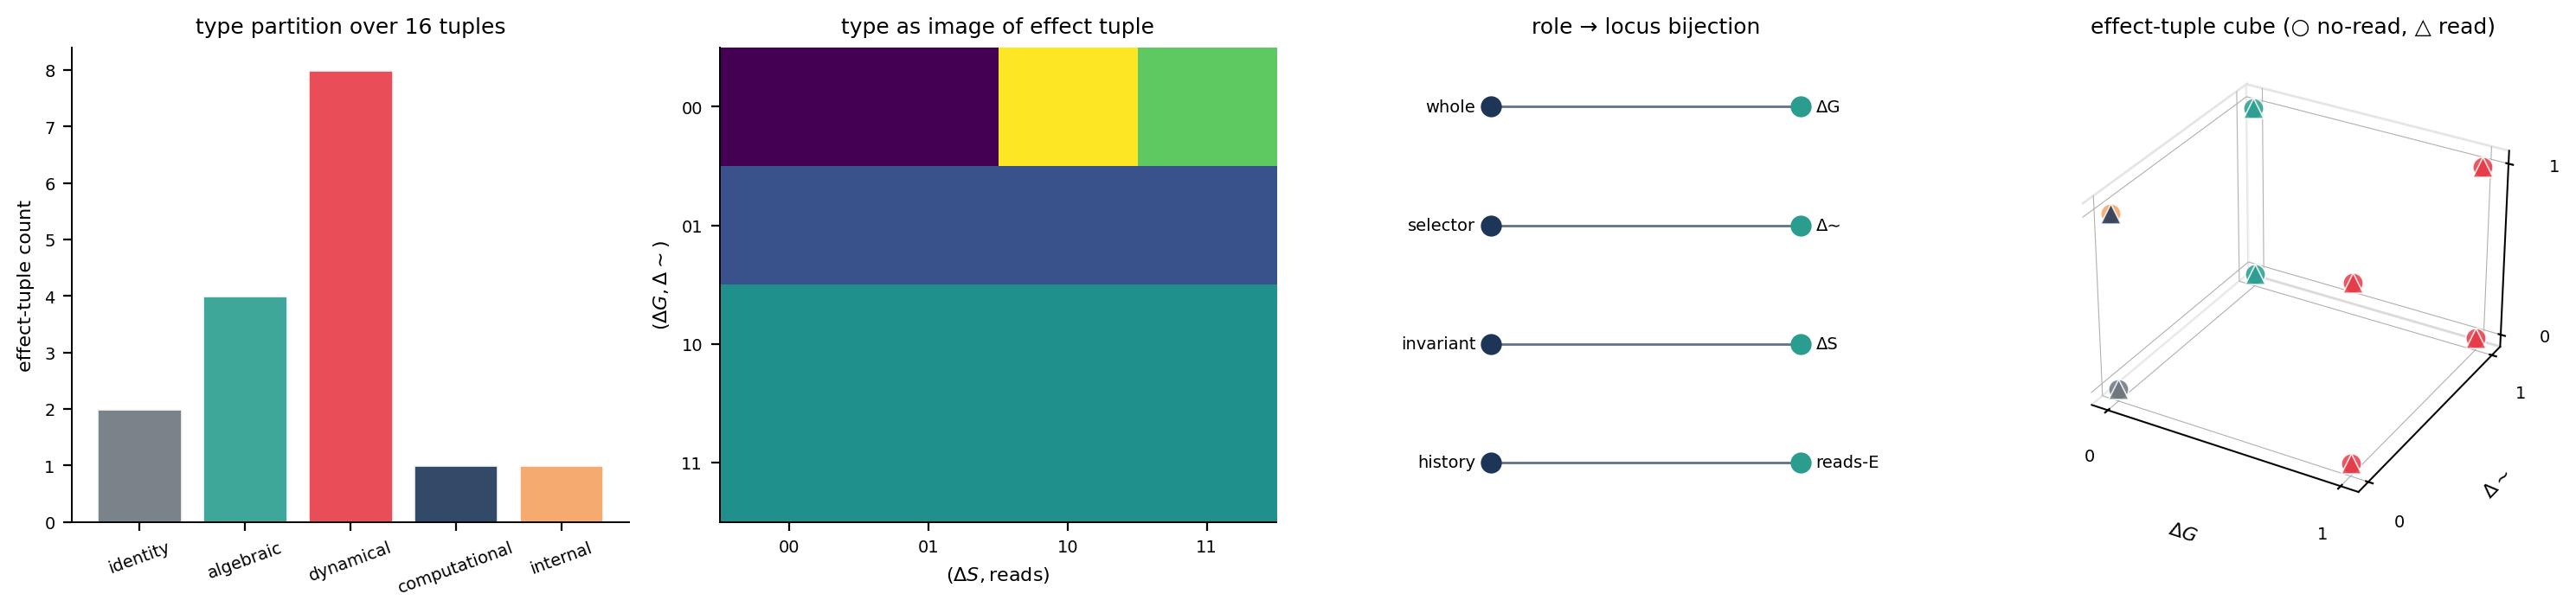
\includegraphics[width=\textwidth]{figures/panel_08_scale_homomorphism.png}
    \caption{\textbf{Scale Homomorphism: Four Roles Surface as Four Loci.}
    (\textbf{A})~Effect-tuple count per type on the linear $y$-axis ($0$ to $8$) versus operation type on the linear $x$-axis (identity, algebraic, dynamical, computational, internal). Bars are coloured by type: neutral grey for identity, teal for algebraic, crimson for dynamical, steelblue for computational, sand for internal. Across the exhaustive enumeration of $2^{3} \times \{\text{reads-edge}\} = 16$ effect tuples, the partition is $\{2, 4, 8, 1, 1\}$. Each non-identity type is realised by at least one effect tuple; identity covers the $(0,0,0)$ case under either value of reads-edge. Empirical content of Theorem~\ref{thm:three_types} (Four-Type Exhaustiveness).
    (\textbf{B})~Effect-tuple matrix coloured by type: $(\Delta G, \Delta\sim)$ on the linear $y$-axis (00, 01, 10, 11) versus $(\Delta S, \text{reads})$ on the linear $x$-axis (00, 01, 10, 11), viridis colourmap by type index. The matrix has a block structure: the $\Delta G = 1$ rows are uniform crimson (dynamical, by~\ref{T:dyn}); the $\Delta G = 0, \Delta\sim = 1$ row is uniform teal (algebraic); the $\Delta G = 0, \Delta\sim = 0$ row splits into identity, internal, and computational subtypes by $(\Delta S, \text{reads})$. Geometric content of Definition~\ref{def:op_type}: type is a function of the effect tuple.
    (\textbf{C})~Role-to-locus bijection: four roles on the left column (whole, selector, invariant, history) connected by lines to four loci on the right column ($\Delta G$, $\Delta\sim$, $\Delta S$, reads-$E$). Each role maps to exactly one locus; the assignment is a bijection. Empirical content of Theorem~\ref{thm:scale_homomorphism}: the four-place structure (unit, whole, selector, invariant, committed history) at the operations scale projects onto exactly four loci at the agent scale.
    (\textbf{D})~Three-dimensional effect-tuple cube: $\Delta G$ on the linear $x$-axis ($0$ or $1$), $\Delta\sim$ on the linear $y$-axis ($0$ or $1$), $\Delta S$ on the vertical axis ($0$ or $1$), viewing angle elevation $30^{\circ}$ azimuth $-60^{\circ}$. Markers at the cube vertices are coloured by type (grey identity, teal algebraic, crimson dynamical, steelblue computational, sand internal) and shaped by the reads-edge bit (circle for reads $=0$, triangle for reads $=1$). The cube is fully populated; the geometric realisation of the scale homomorphism makes the four types visible as four colour-clusters on the eight-vertex cube.}
    \label{fig:panel-scale-homomorphism}
\end{figure*}

\begin{figure*}[!htbp]
    \centering
    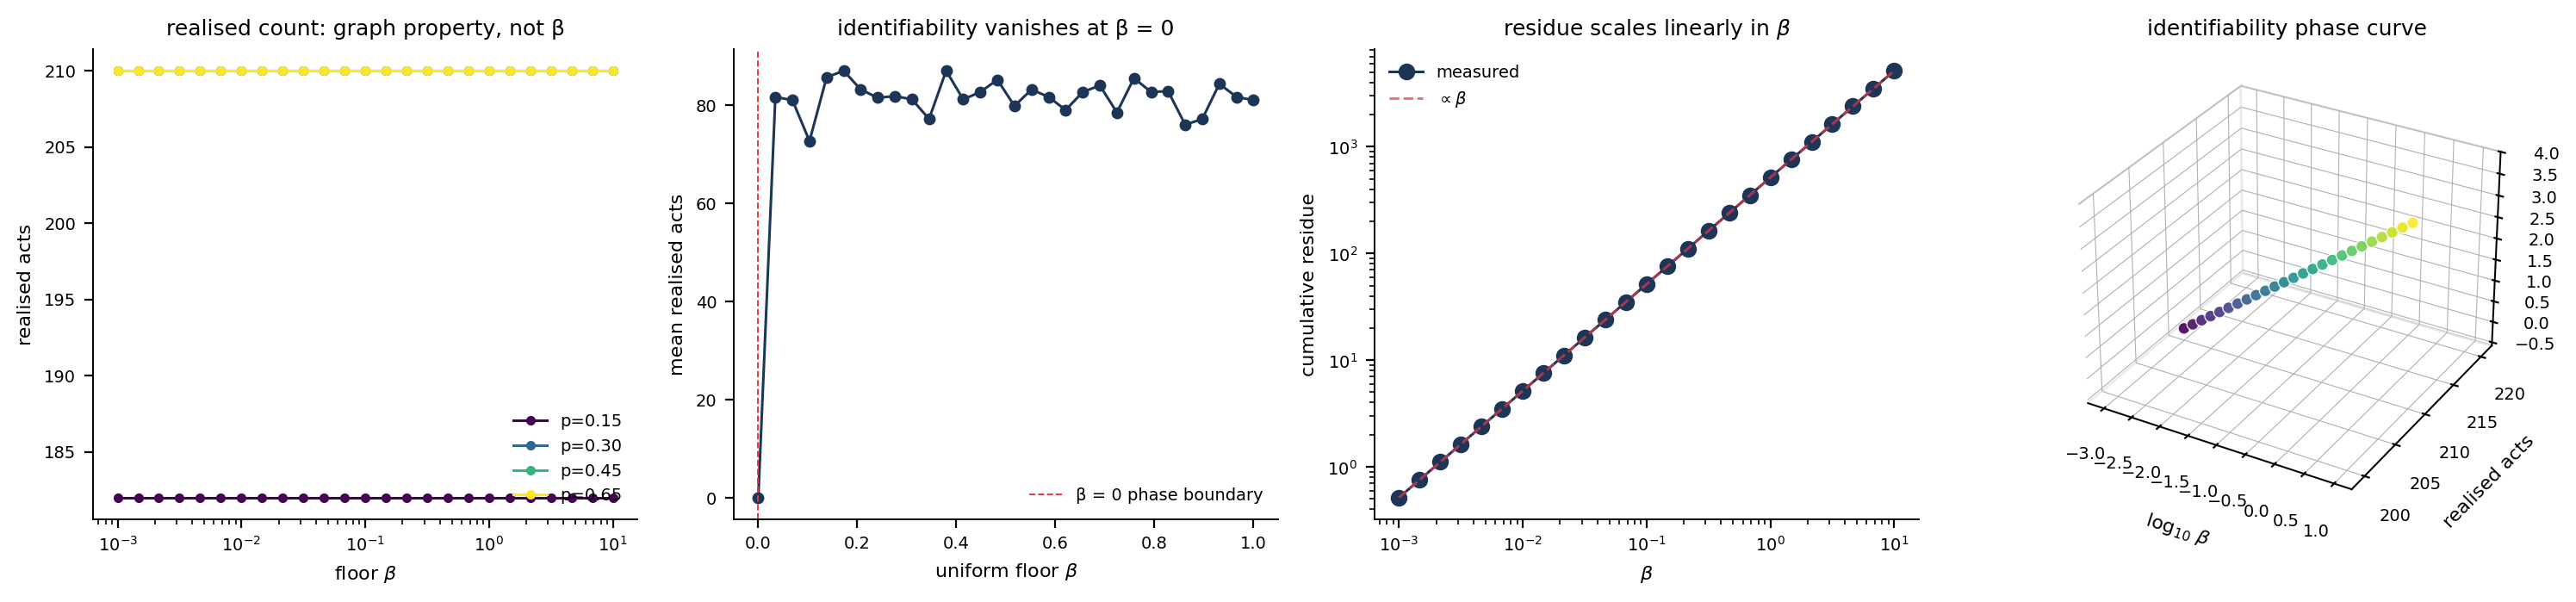
\includegraphics[width=\textwidth]{figures/panel_09_master.png}
    \caption{\textbf{Master Theorem: Identifiability and Operational Structure are Equivalent.}
    (\textbf{A})~Realised acts on the linear $y$-axis ($\sim 170$ to $\sim 215$) versus floor $\beta$ on a log $x$-axis ($10^{-3}$ to $10^{1}$). Four viridis-coloured curves correspond to four fixed graph topologies of edge density $p \in \{0.15, 0.30, 0.45, 0.65\}$, with $\beta$ swept as a uniform edge-weight scale factor. Each curve is constant in $\beta$ across five decades: the realised-act count is a structural property of the graph, independent of the floor. This is the empirical content of Corollary~\ref{cor:identifiability_is_structure}: identifiability is a property of $(\mathcal{A}, \mathcal{G})$, while $\beta$ controls only the cost of realising it.
    (\textbf{B})~Mean realised acts (averaged over $12$ random replicas per $\beta$) on the linear $y$-axis ($0$ to $\sim 90$) versus uniform floor $\beta$ on the linear $x$-axis ($0$ to $1.0$). Steelblue circles trace the mean; the crimson dashed reference at $\beta = 0$ marks the phase boundary. The mean drops abruptly from $\sim 80$ at $\beta > 0$ to exactly $0$ at $\beta = 0$. Empirical content of the contrapositive of Theorem~\ref{thm:master}: setting $\beta = 0$ (denying non-completability, by Corollary~\ref{cor:floor_trace}) dissolves identifiability; no realisable distinguishability act exists.
    (\textbf{C})~Cumulative residue on a log $y$-axis ($10^{-1}$ to $10^{2}$) versus $\beta$ on a log $x$-axis ($10^{-3}$ to $10^{1}$) for the fixed-topology sweep. Steelblue circles trace the measured cumulative residue $\sum\rho_i$; the crimson dashed reference line $\sum\rho_i \propto \beta$ has slope $1$ in log-log coordinates. Measured and theoretical curves coincide across five decades, confirming that cumulative residue scales linearly with the floor and the realised-act count is structural.
    (\textbf{D})~Three-dimensional identifiability phase curve: $\log_{10}\beta$ on the linear $x$-axis ($-3$ to $1$), realised acts on the linear $y$-axis ($\sim 200$ to $\sim 220$), $\log_{10}\sum\rho_i$ on the vertical axis ($-1$ to $4$), viridis colourmap by $\log_{10}\beta$, viewing angle elevation $30^{\circ}$ azimuth $-60^{\circ}$. The curve is monotone in $\log\beta$ and $\log\sum\rho_i$ while flat in realised-act count: the structure is invariant in the agent-graph topology, and the cost surface rises linearly with the floor. Geometric realisation of the three-way equivalence (i) $\Leftrightarrow$ (ii) $\Leftrightarrow$ (iii) of Theorem~\ref{thm:master}.}
    \label{fig:panel-master}
\end{figure*}
